%% Springer Nature LaTeX template
%% For journal articles
\documentclass[sn-mathphys-num]{sn-jnl}

%%% Patches for sn-jnl.cls compatibility
\usepackage{manyfoot}
\usepackage{xcolor}
\providecommand{\jyear}[1]{\gdef\@jyear{#1}}

%%% Packages
\usepackage{graphicx}
\usepackage{multirow}
\usepackage{amsmath,amssymb,amsfonts}
\usepackage{amsthm}
\usepackage{mathrsfs}
\usepackage{booktabs}
\usepackage{hyperref}
\usepackage{enumitem}
\usepackage{pifont}
\usepackage{appendix}
\usepackage{tikz}
\usetikzlibrary{arrows.meta, positioning, calc, fit, backgrounds,
  decorations.pathreplacing, patterns}

%%% Geometry override
\geometry{bindingoffset=0mm, left=25mm, right=25mm, top=25mm, bottom=30mm, headsep=6mm, footskip=10mm}

%%% Theorem environments
\theoremstyle{definition}
\newtheorem{definition}{Definition}[section]
\newtheorem{theorem}{Theorem}[section]
\newtheorem{corollary}{Corollary}[section]
\newtheorem{proposition}{Proposition}[section]
\newtheorem{remark}{Remark}[section]

%%% Custom commands
\newcommand{\Hab}{H^{\mathrm{ab}}}
\newcommand{\ICO}{\mathrm{ICO}}
\newcommand{\Forb}{\mathrm{Forb}}
\newcommand{\tr}{\mathrm{tr}}

%%%% Journal metadata (adjust as needed)
\jyear{2026}

\begin{document}

\title[A5 and the Algebraic Origin of Information Barriers]{%
Non-Solvability as a Physical Principle:\\
$A_5$ and the Algebraic Origin of Information Barriers}

\author*[1]{\fnm{Masaru} \sur{Numagaki}}\email{m.numagaki@medcure.co.jp}

\affil[1]{\orgname{Independent Researcher}, \orgaddress{\city{Kumamoto}, \country{Japan}}}

\abstract{%
We consider a restricted model class in which microscopic three-dimensional
geometry admits a finite rotation holonomy group $H \le \mathrm{SO}(3)$,
and ask whether $H$ can be uniquely determined from physical postulates alone.

Three postulates---Finiteness~(H1), Irreducibility~(H2),
and Perfectness~(H3)---motivated respectively by
Planck-scale discreteness, the absence of privileged directions,
and the absence of universal abelian charges,
select $A_5$ (the icosahedral rotation group of order~60)
as the unique admissible holonomy under Klein's classification.
Five logically independent sufficient conditions converge
on the same conclusion,
and the entire derivation chain is formally verified in Lean~4
(\texttt{sorry\,=\,0}, \texttt{axiom\,=\,0}).

The central result is not a derivation of the Standard Model,
but a specification of falsifiable structural constraints.
The representation theory of $A_5$ yields a threefold
prohibition structure defined by three independent mechanisms:
a tensor-product selection rule for the four-dimensional irreducible
representation~$\rho_4$~(P1),
a multiplicity-free exclusion principle~(P2),
and a Coxeter-exponent filter derived from the exceptional Lie algebra~$E_8$
via the McKay correspondence~(P3)---that pre-specifies the forbidden
$\varphi$-power exponents $\{9,15,16,25\}$ with explicit algebraic reasons.

As a proof of concept, the pure $\mathrm{SU}(3)$ Yang--Mills
one-loop coefficient $\beta_0 = 11$ is reconstructed
from icosahedral cell data as the identity $V - 1 \equiv E/n + \chi/2$,
a Type~I (renormalization-group-invariant, hereafter RG-invariant) quantity
immune to the scale problem.
The scale problem is addressed by classifying RG survival mechanisms
into Type~I--III, with main-text claims restricted to Type~I.
}

\keywords{%
$A_5$,
finite holonomy,
Klein classification,
prohibition structure,
McKay Correspondence,
Information barriers
}

\maketitle

\tableofcontents

%% ============================================================
%% SECTION 1: Introduction
%% ============================================================
\section{Introduction}\label{sec:introduction}

\subsection{Motivation and scope}\label{sec:motivation}

This paper investigates a restricted model class in which microscopic geometry
in three spatial dimensions admits a finite rotation holonomy $H \leq
\mathrm{SO}(3)$, and asks: can $H$ be uniquely determined by physical
principles alone---without fitting to empirical data?

The central question is whether the following logical chain is valid:
\begin{equation}\label{eq:logical-chain}
  \text{Principles} \;\longrightarrow\; \text{Classification}
  \;\longrightarrow\; \text{Uniqueness.}
\end{equation}

The conclusion is conditional. As long as (H1)--(H3) are adopted, $H \cong
A_5$ remains unique within the framework of the Klein classification (Main
Theorem). On the other hand, we do not claim to derive the Standard Model
(SM) directly. Instead, the representation theory of $A_5$ yields a
\emph{prohibition structure} (also called the \emph{index system} or the
\emph{exponent system} in earlier drafts): a pre-specification of ``what must
not appear'' as a falsifiable constraint, determining which $\varphi$-power
exponents are permitted and which are forbidden.
Throughout this paper, the term \emph{prohibition structure} is used
exclusively.

The SM has more than 19 free parameters and does not explain why they take
the values they do. The position of this paper is not to deny the SM, but to
interpret it as a low-energy effective description of physics generated by the
algebraic rigidity of $A_5$, and to argue against the fundamental existence of
free parameters.

\medskip
\noindent\textbf{Limitations.}
The $A_5$ holonomy in this paper is a constraint on the exterior space and
does not directly determine the interior gauge symmetry. The
exterior--interior connection, the construction of the action functional, and
the emergence of the continuum limit are addressed in Open Problem~G1$'$
(Sect.~\ref{sec:limitations}, Appendix~F).


\subsection{Contributions (three core claims)}\label{sec:contributions}

The contributions of this paper are limited to the following three claims.

\medskip
\noindent\textbf{Claim~1: Conditional uniqueness (Layer P $\to$ M).}
We formulate three postulates---finiteness (H1), irreducibility (H2), and
perfectness (H3)---under independent motivation and show that $A_5$ is the
only admissible holonomy selected by Klein's classification of finite rotation
groups (Theorem~\ref{thm:main}). Furthermore, we show that five logically
independent sufficient conditions converge to the same conclusion
(Corollaries~\ref{cor:solvable-opacity}--\ref{cor:fivefold}), ensuring the
robustness of the conclusion (resistance to arbitrariness). This entire chain
of reasoning is formally verified in Lean~4.

\medskip
\noindent\textbf{Claim~2: Minimal physical bridge (Type~I proof of concept).}
As a Type~I quantity independent of the RG scale, we reconstruct the pure
$\mathrm{SU}(3)$ Yang--Mills $\beta_0 = 11$ from the icosahedral data
(Sect.~\ref{sec:beta0}). The identity $V - 1 \equiv E/n + \chi/2$ eliminates
arbitrariness in the choice of formula.

\medskip
\noindent\textbf{Claim~3: Falsifiable prohibition structure (Layer~E core).}
From $A_5$ representation theory---the $\rho_4$ selection rule, the
multiplicity-free condition, and the $E_8$ filter via McKay---the
$\varphi$-exponents appearing in dimensionless constants are sorted into
allowed and prohibited ranges (Sect.~\ref{sec:prohibition}). The $\mathrm{gap} =
1/\varphi^3$ is a quantity derived representation-theoretically from the
character table (Sect.~\ref{sec:algebraic-data}) and has no free parameters
outside of $A_5$. What is important is not the ``enumeration of matches'' but
the falsification form: ``reject if the observed exponent falls within the
forbidden index $\{9, 15, 16, 25\}$.''

Other aspects---the exhaustive agreement of the constants table, the
completion of the dynamical emergence to the SM, and detailed calculations of
the frozen hypothesis along the history of the universe---are clearly
separated as open problems (Sect.~\ref{sec:limitations}). Matters beyond the
scope of this paper (such as the derivation of the SM, the dynamical
mechanism, and the numerical proximity beyond chance in Appendix~A) are
explicitly listed in Sect.~\ref{sec:not-claimed}.


\subsection{Epistemic contract: Layer M / P / E}\label{sec:epistemic}

To avoid confusion, the arguments in this paper are divided into three
layers, and all subsequent discussions are governed by this contract.

\begin{table}[ht]
\caption{Three layers of epistemological separation.}\label{tab:layers}
\centering
\small
\begin{tabular*}{\textwidth}{@{\extracolsep{\fill}}p{2.2cm}p{3.8cm}p{3.5cm}p{3.8cm}@{}}
\toprule
Layer & Content & Verification method & Subject to refutation \\
\midrule
Layer~M (Mathematical theorems)
  & Theorem~\ref{thm:opacity},
    Corollaries~\ref{cor:degeneracy}--\ref{cor:cumulative},
    Theorem~\ref{thm:main},
    Corollaries~\ref{cor:solvable-opacity}--\ref{cor:fivefold},
    representation-theoretic calculations
  & Lean~4 + Mathlib ($\mathtt{sorry} = 0$, $\mathtt{axiom} = 0$)
  & Cannot be disproved (guaranteed by the type checker) \\
\midrule
Layer~P (Physical assumptions)
  & (H1) finite holonomy, (H2) irreducibility, (H3) perfectness
  & Theoretical consistency and indirect empirical evaluation
  & ``Does nature belong to this model class?'' \\
\midrule
Layer~E (Empirical correspondence)
  & Physical realization of prohibition structure, correspondence between
    allowed exponents and experimental values
  & Future precision measurements and new experiments
  & ``Is the algebra of $A_5$ reflected in physical constants?'' \\
\bottomrule
\end{tabular*}
\end{table}

This separation ensures that criticism of each layer does not spread to other
layers. Even if the numerical proximity of Layer~E turns out to be accidental,
the theorems of Layer~M and the conditional propositions of Layer~P are not
affected. Conversely, even if the assumptions of Layer~P are empirically
rejected, the mathematical content of Layer~M continues to hold independently.

\medskip
\noindent\textbf{The position of formal verification.}
The mathematical reasoning in this paper---from the three principles to the
uniqueness of $A_5$ and the entire process leading to the
representation-theoretic consequences---has been machine-verified using Lean~4
\cite{Lean4} + Mathlib \cite{Mathlib} ($\mathtt{sorry} = 0$,
$\mathtt{axiom} = 0$). This allows criticism to focus on (a) the correctness
of the Lean~4 type checker itself, or (b) the physical validity of the three
principles. The theorem--Lean identifier correspondence table is included in
the GitHub repository.


\subsection{Falsifiability at a glance: what would refute this paper}%
\label{sec:falsifiability}

The claims in this paper are separated into three layers (Layer~M/P/E) with
different modes of refutation.

\subsubsection*{(i) Layer~M (irrefutable)}

The theorems in Sect.~\ref{sec:main-theorem} and the algebraic facts in
Sect.~\ref{sec:prohibition} (character tables, tensor product decomposition, and
prohibition structures) do not depend on empirical facts. What can be
disproved is the Layer~P/E hypothesis that ``the mathematics is reflected in
nature.''

\subsubsection*{(ii) Layer~P (falsification of the postulates)}

(H1)--(H3) can be rejected independently. (H1) is refuted by evidence that
the microscopic holonomy is a continuous group, (H2) by the existence of a
universal fixed axis, and (H3) by the existence of a universal discrete
charge. Detailed conditions for the refutation of each postulate are given in
Sects.~\ref{sec:H1}--\ref{sec:H3}.

\subsubsection*{(iii) Layer~E (most important: prohibition structure)}

The core of our empirical argument is not an enumeration of coincidences but
a \emph{prohibition structure}. A selection rule derived from $A_5$
representation theory cuts off the allowable range of $\varphi$-power
exponents, prohibiting a specific set of exponents: $\{9, 15, 16, 25\}$. If
future precision measurements reveal that stable dimensionless ratios have
$\varphi^p$ relations corresponding to these prohibited exponents, the
prohibition structure is immediately rejected.

\medskip
\noindent\textbf{Specific scenarios.}
(a) The system would be refuted if the absolute value of the neutrino mass
ratio is determined (e.g.\ by DUNE) and the exponent $p$ of
$m_{\nu_3}/m_{\nu_2}$ falls within the forbidden set.
(b) It would also be refuted if the discovery of fourth-generation charged
leptons is inconsistent with the constraints derived from McKay--$E_8$.
(c) If the Higgs self-coupling constant $\lambda_H$ is precisely measured
after LHC Run~3 and the deviation from the ICO value is established at
$5\sigma$, its application to the electroweak sector would be rejected.

These scenarios are hypothetical, but the prohibition structure specifies
clear rejection criteria in advance. In this respect, it is qualitatively
different from fitting numbers after the fact.

\subsubsection*{(iv) Layer~E (subsidiary)}

The individual ICO values in Appendix~A will be individually tested by future
precision measurements, but the $A_5$ uniqueness in
Sect.~\ref{sec:main-theorem} and the prohibition structure (the algebra itself) in
Sect.~\ref{sec:prohibition} will not be affected.

\subsubsection*{(v) Logical structure of refutation}

\begin{itemize}[nosep]
  \item Layer~M collapse $\leftarrow$ Lean~4 type checker bug (effectively
    eliminated).
  \item Layer~P collapse $\leftarrow$ (H1) $\lor$ (H2) $\lor$ (H3) is
    rejected $\to$ the premise of the conditional theorem is lost.
  \item Layer~E collapse $\leftarrow$ violation of the prohibited index or
    significant deviation from numerical proximity $\to$ Layer~M / Layer~P
    are not affected.
\end{itemize}


\subsection{Paper organization}\label{sec:organization}

The structure of this paper is as follows.

In Sect.~\ref{sec:postulates}, we formulate the model class and three postulates
(H1)--(H3), and clarify the physical motivation and falsification conditions
for each postulate. In Sect.~\ref{sec:main-theorem}, we prove the main theorem
(the uniqueness of $A_5$) and verify its robustness using five independent
convergence conditions. In Sect.~\ref{sec:beta0}, we present the icosahedral
reconstruction for $\beta_0 = 11$ as a proof of concept, establishing the
privileged status of Type~I invariants. In Sect.~\ref{sec:scale-problem}, we
directly address the scaling problem (G2) and clarify the scope of our claims
through a Type~I/II/III classification. In Sect.~\ref{sec:prohibition}, we
present the prohibition structure and derive the
allowed/forbidden exponents using three layers: the $\rho_4$ selection rule,
the multiplicity filter, and the $E_8$ Coxeter-exponent filter. In
Sect.~\ref{sec:limitations}, we discuss limitations, compare with previous
research, and organize open problems G1$'$--G6 into a prioritized research
agenda. In Sect.~\ref{sec:conclusion}, we draw conclusions. Appendix~A contains
protocolized observation logs (including A.12~Audit Summary) conforming to
rules (R1)--(R3).


%% ============================================================
%% Placeholder labels for forward references
%% (to be replaced when subsequent sections are added)
%% ============================================================

%% ============================================================
%% SECTION 2: Model Class and Postulates
%% ============================================================
\section{Model Class and Postulates}\label{sec:postulates}

In this section, we define the model class under consideration and formulate
three postulates (H1)--(H3), each of which is independently motivated and
immediately followed by a falsification condition.

\subsection{Defining the model class}\label{sec:model-class}

This paper does not claim conclusions derived from general quantum gravity. We
first state the limitation explicitly: the model class is restricted to those
in which the micro-holonomy of the external space is expressed by a finite
rotation group.

Discrete rotational symmetries in three-dimensional space have been completely
classified by Klein~\cite{Klein1884}; see also Burnside~\cite{Burnside1911}
for the classical theory of finite groups. The finite subgroups of
$\mathrm{SO}(3)$ fall into five families: the cyclic group $C_n$, the dihedral
group $D_n$, the tetrahedral group $A_4$ (order~12), the octahedral group
$S_4$ (order~24), and the icosahedral group $A_5$ (order~60).

The question in this paper is: \emph{Can one of these five candidates be
uniquely selected using only physically independent principles?}

\medskip
\noindent\textbf{The unifying motivation of the three principles: information
finiteness.}
The three principles are not independent and arbitrary assumptions. They are
positioned as stepwise constraints naturally motivated by the
information-theoretic requirement that ``microscopic geometry at the Planck
scale can only hold a finite amount of information.'' The finiteness of
information motivates the reduction from continuous groups to finite groups
(H1), the isotropic maximal utilization of finite degrees of freedom requires
the absence of privileged directions (H2), and the fact that the information
barrier collapses to zero in solvable groups (Theorem~\ref{thm:opacity})
makes non-solvability inevitable (H3).

Each stage adds independent physical content---(H2) assumes an isotropic
information distribution in space, and (H3) assumes the existence of
irreversibility---but they are all motivated by the common requirement of
finite information, which is consistent with the Bekenstein upper
bound~\cite{Bekenstein73}, the holographic principle, and several quantum
gravity programs (Regge calculus~\cite{Regge61}, CDT~\cite{CDT},
spin foam~\cite{SpinFoamA,SpinFoamB}).


\subsection{Postulate (H1): Finite holonomy (model class definition)}%
\label{sec:H1}

\noindent\textbf{Statement.}
Microscopic local geometry has a finite subgroup $H \leq \mathrm{SO}(3)$ as
its holonomy group:
\begin{equation}\label{eq:H1}
  H \leq \mathrm{SO}(3),\qquad |H| < \infty.
\end{equation}

\noindent\textbf{Physical motivation.}
(H1) is a model class-defining assumption, motivated by the natural emergence
of discrete holonomies in discrete quantum gravity approaches (Regge
calculus~\cite{Regge61}, CDT~\cite{CDT}, spin
foam~\cite{SpinFoamA,SpinFoamB}), the finite information property due to the
Bekenstein upper bound~\cite{Bekenstein73}, and the nontrivial physical
content of finite group lattice gauge theory~\cite{FinLGT}.

\medskip
\noindent\textbf{Operational definition.}
In the three-dimensional Regge lattice, we assign an element $g_e \in H$ to
the deficit angle of the triangle enclosing edge $e$ in $\mathrm{SO}(3)$, and
specify the geometric situation in which the range of the holonomy
$h_\gamma = \prod_{e \in \gamma} g_e$ along a closed curve $\gamma$ is
restricted to a finite group.

\medskip
\noindent\textbf{What (H1) precludes.}
Continuous rotation groups only. Klein's classification limits the number of
candidates to five.

\medskip
\noindent\textbf{Dimensional dependence.}
The choice of $n = 3$ is nontrivial. For $n = 2$ ($\mathrm{SO}(2)$), the only
finite subgroups are the cyclic groups $C_m$, and there are no non-solvable
finite rotation groups, so the elimination method using (H2)(H3) itself fails.
For $n = 4$ ($\mathrm{SO}(4)$), the finite subgroups become enriched, making
it difficult to achieve uniqueness via (H3). The gap $= 1/\varphi^4 \approx
0.146$ leads to $\alpha_s = \mathrm{gap}/2 = 0.073$ (a 38\% deviation from
the experimental value of $0.1180$). $n = 3$ is a necessary condition for the
gap $= 1/\varphi^3$ to be consistent with $\alpha_s(M_Z)$ within $0.03\%$.

\medskip
\noindent\textbf{Refutation condition.}
Conclusive evidence that the microscopic holonomy is a continuous
group---direct observation of quantum gravitational effects without discrete
rotational symmetry---would eliminate (H1). Indirectly, evidence for $n \neq
3$ also weakens (H1) (see quantitative collapse above).

\medskip
\noindent\textbf{Clarification of scope.}
This paper restricts itself to the holonomy of space frame bundles, excluding
the spacetime holonomy ($\mathrm{Lorentz}/\mathrm{Spin}(3,1)$). The lifting
to $\mathrm{Spin}(3) \cong \mathrm{SU}(2)$ is treated as the binary
icosahedral group $2I$ in Sect.~\ref{sec:prohibition}.


\subsection{Postulate (H2): Irreducibility (absence of locally privileged
directions)}\label{sec:H2}

\noindent\textbf{Statement.}
The natural action of $H$ on $\mathbb{R}^3$ is irreducible:
\begin{equation}\label{eq:H2}
  \mathbb{R}^3 \;\text{is irreducible as an $H$-module.}
\end{equation}

\noindent\textbf{Physical motivation.}
(H2) encodes the absence of locally privileged directions. When $H$ acts
reducibly, the invariant subspace defines a ``special axis that is fixed in
all microscopic rotations.'' (H2) eliminates the inherent anisotropy at this
microscopic level, and is a stronger requirement independent of the
statistical isotropy of random orientations (macro-isotropy).

\begin{table}[ht]
\caption{(H2) eliminates $C_n$ and $D_n$; the polyhedral groups
$\{A_4, S_4, A_5\}$ survive.}\label{tab:H2}
\centering
\begin{tabular*}{\textwidth}{@{\extracolsep{\fill}}lccc@{}}
\toprule
Group & 3D representation & Invariant subspace & (H2) \\
\midrule
$C_n$ ($n \geq 2$) & Reducible & Rotation axis (1-dim.) & \ding{55} \\
$D_n$               & Reducible & Main axis (1-dim.)     & \ding{55} \\
$A_4,\; S_4,\; A_5$ & Irreducible & None                 & \ding{51} \\
\bottomrule
\end{tabular*}
\end{table}

\noindent\textbf{Refutation condition.}
If a universal fixed axis can be definitively confirmed at the single-cell
level, then (H2) is rejected. If (H2) is violated, the five-fold symmetry
disappears, $\varphi$ disappears from the character table, and the entire
prohibition structure of Sect.~\ref{sec:prohibition} collapses.


\subsection{Postulate (H3): Perfectness (absence of universal abelian
charges)}\label{sec:H3}

\noindent\textbf{Statement.}
The abelianization of the holonomy group $H$ is trivial:
\begin{equation}\label{eq:H3}
  \Hab = H/[H,\,H] = 1.
\end{equation}

\noindent\textbf{Physical motivation.}
(H3) is the principle that ``there is no universally definable abelian charge
from microscopic holonomy.'' The sign homomorphism of $S_4$ automatically
imparts a $\mathbb{Z}_2$ charge, and the quotient map $A_4 \to C_3$ of $A_4$
automatically imparts a $\mathbb{Z}_3$ charge. (H3) excludes this kind of
automatically existing abelian conserved quantity.

\medskip
\noindent\textbf{Connections with symmetry constraints in quantum gravity.}
(H3) is structurally parallel to the No-Global-Symmetries Conjecture
(Banks--Dixon~\cite{BanksDixon}; Harlow--Ooguri~\cite{HarlowOoguri}) and the
Cobordism Conjecture (McNamara--Vafa~\cite{McNamaraVafa}). The discrete
charges automatically defined from $\Hab \neq 1$ are nothing but discrete
counterparts of the global symmetries eliminated in quantum gravity. However,
both conjectures remain unproven, and strict equivalence with (H3) has not
been established. This paper treats (H3) as an independent physical principle.

\medskip
\noindent\textbf{Structural alignment with Swampland conditions.}
The $A_5$ holonomy automatically satisfies the key conditions of the Swampland
program---No-Global-Symmetries, Cobordism, Distance, and
Finiteness---in a structural way. $\Hab = 1$ forbids discrete global
symmetries, and the absence of a continuous moduli space for discrete
holonomies renders the assumption of the Distance Conjecture inapplicable. A
systematic comparison is given in Appendix~C.5.

\begin{table}[ht]
\caption{(H3) eliminates $A_4$ and $S_4$; only $A_5$
survives.}\label{tab:H3}
\centering
\begin{tabular*}{\textwidth}{@{\extracolsep{\fill}}lccc@{}}
\toprule
Group & $\Hab$ & Automatic charge & (H3) \\
\midrule
$A_4$ & $C_3$  & $\mathbb{Z}_3$ charge & \ding{55} \\
$S_4$ & $C_2$  & $\mathbb{Z}_2$ sign   & \ding{55} \\
$A_5$ & $1$    & None                   & \ding{51} \\
\bottomrule
\end{tabular*}
\end{table}

\noindent\textbf{Refutation condition.}
At the microscopic level, if the existence of a universal discrete charge
($\mathbb{Z}_2$ sign or $\mathbb{Z}_3$ phase) is confirmed, (H3) is
disproved. If (H3) is violated and $A_4$ is adopted, $\alpha^{-1} \approx
27.4$ (80\% deviation), $\Omega_{\mathrm{DM}}/\Omega_b = 3$ (43\% deviation).

\medskip
\noindent\textbf{(H3) enhancement: solvable opacity (H3*).}
As we show in Sect.~\ref{sec:solvable-opacity}, (H3) is only the weakest shadow
of the solvable probe analysis. A stronger property, (H3*), holds: any
homomorphism from $A_5$ to a solvable group is trivial. On the candidate set
$\{A_4, S_4, A_5\}$, (H3) and (H3*) are equivalent, but (H3*) has a wider
scope as a physical principle.

\medskip
\noindent\textbf{Consistency with effective $\mathrm{U}(1)$.}
(H3) does not deny low-energy $\mathrm{U}(1)$ symmetry; it only forbids the
group-homomorphic image $H \to \mathrm{U}(1)$. An effective $\mathrm{U}(1)$
appears in the thermodynamic limit with many degrees of freedom.


\subsection{Independence and acyclicity of the three principles}%
\label{sec:independence}

The three motivations are independent: (H1) is based on the definition of a
model class, (H2) on local isotropy, and (H3) on the absence of universal
charge. The exclusions are also non-overlapping---(H2) excludes $C_n$, $D_n$,
and (H3) excludes $A_4$, $S_4$---so the three conditions function without
redundancy. $A_5$ itself is not directly assumed. The fact that there are only
five finite subgroups of $\mathrm{SO}(3)$ due to the Klein classification
makes the uniqueness possible, but this does not occur for any pair of
conditions alone (as will be refined in Sect.~\ref{sec:strengths}).

%% ============================================================
%% SECTION 3: Main Theorem
%% ============================================================
\section{Main Theorem: Uniqueness of \texorpdfstring{$A_5$}{A5} Holonomy
in \texorpdfstring{$\mathrm{SO}(3)$}{SO(3)}}\label{sec:main-theorem}

In this section, we prove that the three principles of Sect.~\ref{sec:postulates}
uniquely select $A_5$ in the Klein classification framework. In the first
half, we briefly demonstrate the solvable opacity behind (H3), and in the
second half, we establish the robustness of the main theorem via alternative
conditions.

\subsection{Solvable opacity}\label{sec:solvable-opacity}

(H3) is the weakest shadow of a solvable probe analysis. To clarify this
structure, the more general results are presented first.

\begin{definition}[Solvable probe]\label{def:solvable-probe}
For a finite group $G$, a \emph{solvable probe} is a group homomorphism
$\pi \colon G \to Q$ to a solvable group $Q$. Physically, a solvable probe
corresponds to an information channel defined by a finite-depth sequential
measurement procedure---a hierarchical composition in which commuting outputs
are used as inputs to select the observations of the next stage.
\end{definition}

\begin{theorem}[Opacity of solvable images]\label{thm:opacity}
Let $G$ be a finite non-solvable group. Any solvable probe
$\pi \colon G \to Q$ is non-injective.
\end{theorem}

\begin{proof}
If $\pi$ is injective, then $G \cong \pi(G) \leq Q$, and by subgroup
inheritance of solvability, $G$ is also solvable---a contradiction.
\emph{[Lean~4 verified.]}
\end{proof}

\begin{corollary}[Complete degeneracy]\label{cor:degeneracy}
Let $G$ be a finite simple group that is non-solvable. Any solvable probe
$\pi \colon G \to Q$ is trivial: $\ker(\pi) = G$. For $G = A_5$,
$|\ker(\pi)| = 60$.
\emph{[Lean~4 verified.]}
\end{corollary}

\begin{corollary}[Cumulative opacity]\label{cor:cumulative}
The product map of a finite family of solvable probes
$(\pi_i \colon A_5 \to Q_i)_{i=1}^{k}$ is a constant map. No combination of
finitely many solvable probes can distinguish any two elements in $A_5$.
\emph{[Lean~4 verified.]}
\end{corollary}

\begin{theorem}[$A_5$ as a critical point]\label{thm:critical}
All finite groups of order less than $60$ are solvable, and $A_5$ (order~$60$)
is the smallest non-solvable finite group.
\emph{[Lean~4 verified.]}
\end{theorem}

\begin{corollary}[$A_5$ is the minimal basis for the information barrier]%
\label{cor:minimal-barrier}
\begin{enumerate}[nosep,label=(\roman*)]
  \item $|G| < 60 \;\Rightarrow\; G$ is solvable.
  \item $A_5$ is non-solvable and exhibits complete invisibility with
    $|\ker| = 60$.
  \item The $A_5$ barrier grows exponentially to $60^N \geq 2^{5N}$ in $N$
    steps.
\end{enumerate}
\emph{[Lean~4 verified.]}
\end{corollary}

\begin{definition}[Solvable opacity (H3*)]\label{def:H3star}
\textup{(H3*) Solvable opacity.} For a microscopic holonomy group $H$, any
solvable probe $\pi \colon H \to Q$ is non-injective.
\end{definition}

(H3*) is a strict strengthening of (H3) (since abelian groups $\subset$
solvable groups, (H3*) $\Rightarrow$ (H3)). In the candidate set
$\{A_4, S_4, A_5\}$, they are equivalent---$A_4$, $S_4$ are solvable groups,
so the identity map is an injective solvable probe and is eliminated.

\medskip
\noindent\textbf{Where is the novelty?}
Theorem~\ref{thm:opacity} is the contrapositive of ``a subgroup of a solvable
group is solvable'' and is a direct consequence of standard group theory. The
contributions of this section are: (N1) reformulation as a physical principle
(H3*), (N2) systematization of invisibility by combining
Corollaries~\ref{cor:degeneracy}--\ref{cor:cumulative} and
\ref{cor:minimal-barrier}, and (N3) formal verification of the entire proof
chain. The connection to computational complexity (Barrington, Krohn--Rhodes)
is described in Appendix~B.


\subsection{Main theorem}\label{sec:main-thm-statement}

\begin{theorem}[$A_5$ holonomy uniqueness]\label{thm:main}
Under $(\mathrm{H1}) \land (\mathrm{H2}) \land (\mathrm{H3})$,\;
$H \cong A_5$.
\end{theorem}

\begin{proof}
Assume $H \not\cong A_5$. By Klein's classification theorem
\cite{Klein1884}, $H \cong C_n$, $D_n$, $A_4$, or $S_4$. $C_n$ and $D_n$
are reducible, contradicting (H2). $A_4^{\mathrm{ab}} \cong C_3 \neq 1$ and
$S_4^{\mathrm{ab}} \cong C_2 \neq 1$, contradicting (H3). In every case, a
contradiction arises.
\emph{[Lean~4 verified.]}
\end{proof}


\subsection{Robustness: alternative conditions}\label{sec:robustness}

The same conclusion can be reached by replacing (H3) with any of four
logically independent conditions. All of the following arguments assume that
the candidates have been narrowed to $\{A_4, S_4, A_5\}$ by (H2).

\begin{corollary}[Solvable opacity version]\label{cor:solvable-opacity}
$(\mathrm{H1}) \land (\mathrm{H2}) \land (\mathrm{H3*})
\;\Rightarrow\; H \cong A_5$.
Since $A_4$, $S_4$ are solvable, the identity map is an injective solvable
probe and eliminates them.
\emph{[Lean~4 verified.]}
\end{corollary}

\begin{corollary}[Maximality version]\label{cor:maximality}
$(\mathrm{H3'})$: Select the candidate with the highest order. $A_5$ is
selected because $|A_4| = 12 < |S_4| = 24 < |A_5| = 60$.
\end{corollary}

\begin{corollary}[Non-solvability version]\label{cor:nonsolvability}
$(\mathrm{H3''})$: $H$ is non-solvable. $A_4$ and $S_4$ are solvable, so
they are eliminated; only the non-solvable $A_5$ survives.
\emph{[Lean~4 verified.]}
\end{corollary}

\begin{corollary}[Five-fold symmetry version]\label{cor:fivefold}
$(\mathrm{H3'''})$: $H$ contains an element of order~$5$. The element orders
of $A_4$ are $\{1, 2, 3\}$ and those of $S_4$ are $\{1, 2, 3, 4\}$, so they
are excluded. $A_5$ contains an element of order~$5$
(e.g.,~$(1\;2\;3\;4\;5)$).
\emph{[Lean~4 verified.]}
\end{corollary}

\begin{table}[ht]
\caption{Comparison of five conditions. Each eliminates $A_4$ and $S_4$ by an
independent mathematical mechanism, ensuring that $A_5$ selection is
insensitive to axiom choice.}\label{tab:five-conditions}
\centering
\small
\begin{tabular*}{\textwidth}{@{\extracolsep{\fill}}lp{3.2cm}p{3.2cm}p{3.5cm}@{}}
\toprule
Condition & Formal pattern & Physical motivation & Exclusion mechanism \\
\midrule
(H3) Perfectness
  & $\Hab = 1$
  & Absence of universal abelian charges
  & Abelianization test \\
(H3*) Solvable opacity
  & Solvable probes are non-faithful
  & Fundamental limits of sequential measurement
  & Solvability test \\
(H3$'$) Maximality
  & $|H|$ maximal
  & Maximal utilization of microscopic structure
  & Order comparison \\
(H3$''$) Non-solvability
  & $H$ is non-solvable
  & Existence of irreversibility
  & Solvability test \\
(H3$'''$) Five-fold symmetry
  & $\exists\, g \in H,\;\mathrm{ord}(g) = 5$
  & Existence of five-fold rotational symmetry
  & Element-order enumeration \\
\bottomrule
\end{tabular*}
\end{table}


\subsection{Visualizing the elimination}\label{sec:visualization}

The elimination cascade is summarized in Fig.~\ref{fig:cascade}.

\begin{figure}[ht]
\centering
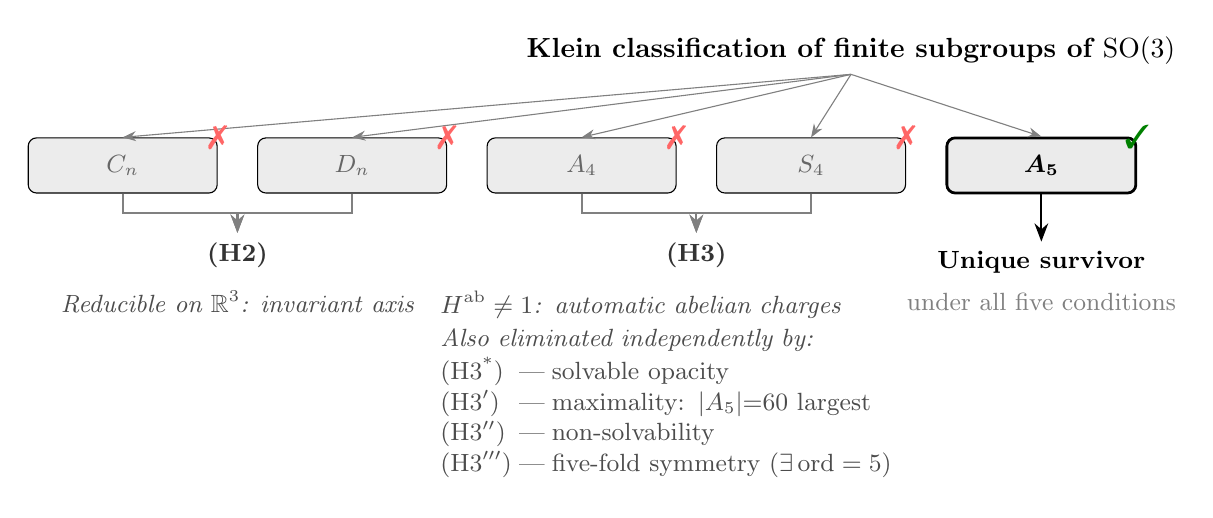
\begin{tikzpicture}[
  >=Stealth,
  node distance=0.6cm and 1.2cm,
  groupbox/.style={
    draw, rounded corners=3pt, minimum width=2.4cm, minimum height=0.7cm,
    font=\small, inner sep=4pt, align=center
  },
  eliminated/.style={groupbox, fill=gray!15, text=black!60},
  survivor/.style={groupbox, fill=black!8, line width=1pt},
  reason/.style={font=\small\itshape, text=black!70, align=left},
  elim-arrow/.style={->, thick, color=black!50},
  postulate/.style={font=\small\bfseries, color=black!80},
]

%%% Top: Klein classification
\node[font=\normalsize\bfseries] (klein)
  {Klein classification of finite subgroups of $\mathrm{SO}(3)$};

%%% Row 1: all five families
\node[eliminated, below left=0.8cm and 3.8cm of klein] (Cn)  {$C_n$};
\node[eliminated, right=0.5cm of Cn]   (Dn)  {$D_n$};
\node[eliminated, right=0.5cm of Dn]   (A4)  {$A_4$};
\node[eliminated, right=0.5cm of A4]   (S4)  {$S_4$};
\node[survivor,   right=0.5cm of S4]   (A5)  {$\boldsymbol{A_5}$};

%%% Arrows from Klein
\foreach \g in {Cn,Dn,A4,S4,A5}{
  \draw[->, thin, gray] (klein.south) -- (\g.north);
}

%%% H2 elimination: Cn, Dn
\node[postulate, below=0.5cm of $(Cn.south)!0.5!(Dn.south)$] (h2label) {(H2)};
\draw[elim-arrow] (Cn.south) -- ++(0,-0.25) -| (h2label);
\draw[elim-arrow] (Dn.south) -- ++(0,-0.25) -| (h2label);
\node[reason, below=0.05cm of h2label] (h2reason)
  {Reducible on $\mathbb{R}^3$: invariant axis};

%%% Cross marks on Cn, Dn
\node[font=\large, color=red!60] at (Cn.north east) {\ding{55}};
\node[font=\large, color=red!60] at (Dn.north east) {\ding{55}};

%%% H3 elimination: A4, S4
\node[postulate, below=0.5cm of $(A4.south)!0.5!(S4.south)$] (h3label) {(H3)};
\draw[elim-arrow] (A4.south) -- ++(0,-0.25) -| (h3label);
\draw[elim-arrow] (S4.south) -- ++(0,-0.25) -| (h3label);

%%% Five alternative reasons
\node[reason, below=0.05cm of h3label, text width=6.5cm] (h3reasons) {%
  $H^{\mathrm{ab}} \neq 1$: automatic abelian charges\\[1pt]
  Also eliminated independently by:\\[1pt]
  \upshape
  \begin{tabular}{@{}l@{\;---\;}l@{}}
  (H3\textsuperscript{*})  & solvable opacity \\
  (H3$'$)  & maximality: $|A_5|{=}60$ largest\\
  (H3$''$) & non-solvability \\
  (H3$'''$)& five-fold symmetry ($\exists\,\mathrm{ord}=5$)
  \end{tabular}};

%%% Cross marks on A4, S4
\node[font=\large, color=red!60] at (A4.north east) {\ding{55}};
\node[font=\large, color=red!60] at (S4.north east) {\ding{55}};

%%% A5 survivor highlight
\node[postulate, below=0.6cm of A5, color=black] (a5label)
  {Unique survivor};
\draw[->, thick] (A5.south) -- (a5label.north);
\node[font=\small, color=black!50, below=0.0cm of a5label]
  {under all five conditions};

%%% Checkmark on A5
\node[font=\large, color=green!50!black] at (A5.north east) {\ding{51}};

\end{tikzpicture}
\caption{Elimination cascade from Klein's classification to $A_5$.
  Postulate (H2) eliminates the cyclic and dihedral groups (reducible action),
  and postulate (H3) eliminates $A_4$ and $S_4$ (nontrivial abelianization).
  Five logically independent conditions all converge on
  $A_5$ as the unique surviving candidate}\label{fig:cascade}
\end{figure}


\subsection{Strengths and limitations of the theorem}\label{sec:strengths}

\noindent\textbf{Strength.}
The elimination consists of the finite candidate property from the Klein
classification, reducible-group exclusion via (H2), and the abelianization
test of (H3); it is completely constructive.
Corollaries~\ref{cor:solvable-opacity}--\ref{cor:fivefold} ensure that five
different conditions converge to the same conclusion, and that the conclusion
is insensitive to the choice of axioms (resistance to arbitrariness).

\medskip
\noindent\textbf{The mathematical nature of the theorem.}
The fact that $A_5$ is the only finite subgroup of $\mathrm{SO}(3)$ that is
both irreducible and perfect is a consequence of the Klein classification and
standard group theory. The contribution of this paper is to reconstruct this
fact as a stepwise elimination based on three independent physical principles.
This provides a framework for evaluating the physical validity of each
assumption individually.

\medskip
\noindent\textbf{Limitation.}
The physical necessity of (H1), (H2), and (H3) cannot be proven. These are
axioms that define a model class of microscopic geometry, and their adoption
is left to theoretical consistency and future empirical investigation.

\medskip
\noindent\textbf{On the smallness of the candidate space.}
The five constraints of the Klein classification make uniqueness
possible---but not self-evident. Non-triviality resides in: (i) the exclusion
targets of (H2)/(H3) being completely non-overlapping, (ii) the convergence of
five independent algebraic characterizations (Sect.~\ref{sec:robustness}), and
(iii) the physical motivation being independent of the conclusion.

\begin{table}[ht]
\caption{No pair of conditions alone suffices within the full physical
framework; all three are needed.}\label{tab:pairs}
\centering
\begin{tabular}{@{}lll@{}}
\toprule
Condition set & Surviving groups & Uniqueness? \\
\midrule
(H1) $\land$ (H2) & $A_4,\; S_4,\; A_5$ & No (3 candidates) \\
(H1) $\land$ (H3) & $C_n,\; D_n,\; A_5$ & No (many candidates) \\
(H2) $\land$ (H3) & $A_5$
  & Yes (but no reason to restrict to finite groups) \\
\bottomrule
\end{tabular}
\end{table}


\subsection{Status of formal verification}\label{sec:verification}

All theorems, corollaries, solvability tests, simplicity proofs, and order
calculations in this section have been formally verified using Lean~4
($\mathtt{sorry} = 0$, $\mathtt{axiom} = 0$). The only unformalized element
is Klein's classification of finite rotation groups \cite{Klein1884},
which is cited as a classical theorem. The correspondence
table is available in the GitHub repository.

%% ============================================================
%% SECTION 4: Proof-of-Concept Bridge
%% ============================================================
\section{Proof-of-Concept Bridge: Reconstructing
\texorpdfstring{$\beta_0 = 11$}{β₀ = 11} from Icosahedral Data}%
\label{sec:beta0}

$H \cong A_5$ is determined by Theorem~\ref{thm:main}. In this section, we
first organize the discrete data derived from $A_5$ in
Sect.~\ref{sec:algebraic-data}, and then reconstruct the one-loop coefficient
$\beta_0 = 11$ of the pure $\mathrm{SU}(3)$ Yang--Mills from the icosahedral
data in Sects.~\ref{sec:why-beta0}--\ref{sec:feedback}, and show that this
agreement is not an arbitrary choice of formula but is structurally necessary.


\subsection{Algebraic data of \texorpdfstring{$A_5$}{A5}: icosahedral
constants, \texorpdfstring{$\varphi$}{φ}, and representation theory}%
\label{sec:algebraic-data}

\subsubsection{Orbit--stabilizer decomposition}\label{sec:orbit-stab}

From the transitive action of
$A_5 \cong \mathrm{Rot}(\text{Icosahedron})$ on geometric elements and
$|A_5| = |\text{Orbit}| \times |\text{Stab}|$:

\begin{table}[ht]
\caption{Orbit--stabilizer decomposition of $A_5$ acting on the
icosahedron.}\label{tab:orbit-stab}
\centering
\begin{tabular*}{\textwidth}{@{\extracolsep{\fill}}llll@{}}
\toprule
Geometric element & Stabilizer & Orbit equation & Value \\
\midrule
Face $F$   & $\mathbb{Z}_3$ & $60/3 = 20$ & 20 \\
Edge $E$   & $\mathbb{Z}_2$ & $60/2 = 30$ & 30 \\
Vertex $V$ & $\mathbb{Z}_5$ & $60/5 = 12$ & 12 \\
\bottomrule
\end{tabular*}
\end{table}

Euler's polyhedron formula $F + V - E = 2$ holds. The triple lock value
$E/n = F/2 = |A_5|/6 = 10$ demonstrates the inherent overdetermination of the
icosahedron. \emph{[Verified.]}

\medskip
\noindent\textbf{Discrete Noether Correspondence (DNC).}
The orbit--stabilizer decomposition uniquely assigns three distinct stabilizer
groups ($\mathbb{Z}_3$, $\mathbb{Z}_2$, $\mathbb{Z}_5$) to three geometric
objects. Each stabilizer group defines topologically conserved discrete quantum
numbers for the closed-curve holonomy and provides an algebraic basis for the
correspondences to the force sectors: faces
($\mathbb{Z}_3$)$\to$electromagnetic, edges
($\mathbb{Z}_2$)$\to$strong force, and vertices
($\mathbb{Z}_5$)$\to$gravitational. However, ab initio derivation of this
correspondence rule (C1) has not yet been achieved (L3, G3), and the choice of
(C1) among the $3! = 6$ possible assignments is a posteriori. The perfectness
(H3) ($\Hab = 1$) prohibits automatic discrete conserved quantities at the
$A_5$ level, while allowing the emergence of effective $\mathrm{U}(1)$
conservation laws in the continuous limit with many degrees of freedom---this
two-layer structure of conservation laws is the physical core of DNC. The
complete formulation of DNC is given in the Appendix.


\subsubsection{Representation-theoretic derivation of \texorpdfstring{$\varphi$}{φ},
Galois deviation rate, and gap}\label{sec:phi-derivation}

\noindent\textbf{Step 1: The occurrence of $\varphi$.}
$A_5$ has five conjugacy classes and the irreducible representation dimensions
$\{1, 3, 3, 4, 5\}$ are determined. The character value
$\chi_{\rho_3}(C_5)$ on the $C_5$ conjugacy class of $\rho_3$ is determined
as a root of the minimal polynomial $x^2 - x - 1 = 0$ by the Schur
orthogonality relation:
\begin{equation}\label{eq:phi}
  \chi_{\rho_3}(C_5) = \varphi = \frac{1 + \sqrt{5}}{2}\,,\qquad
  \chi_{\rho_3}(C_5^2) = -\frac{1}{\varphi} = \frac{1 - \sqrt{5}}{2}\,.
\end{equation}
$\varphi$ is uniquely determined solely from the group structure of $A_5$ and
does not depend on any continuous parameters. \emph{[Verified.]}

\medskip
\noindent\textbf{Step 2: Uniqueness of the Galois deviation rate
$\lambda_\varphi$.}
$\varphi$ and $-1/\varphi$ correspond to the Galois pair
$\mathbb{Q}(\sqrt{5})/\mathbb{Q}$. Define the Galois deviation rate
\begin{equation}\label{eq:lambda}
  \lambda_\varphi := |1 - \varphi| = \varphi - 1
  = \frac{1}{\varphi} \approx 0.618\,.
\end{equation}
As the following exhaustive check shows, $\lambda_\varphi$ is the only
non-trivial coupling parameter that the character table of $A_5$
allows---the only character value satisfying $0 < |\chi| < 1$.

\begin{table}[ht]
\caption{Exhaustive scan of character values. Only $1/\varphi$ on
$\rho_3|_{C_5^2}$ satisfies $0 < |\chi| < 1$.}\label{tab:character-scan}
\centering
\small
\begin{tabular*}{\textwidth}{@{\extracolsep{\fill}}llccc@{}}
\toprule
Repr. & Conj.\ class & $\chi$ & $|\chi|$ & $0 < |\chi| < 1$? \\
\midrule
$\rho_3$ & $C_5$    & $\varphi \approx 1.618$  & $> 1$ & No \\
$\rho_3$ & $C_5^2$  & $-1/\varphi \approx 0.618$ & $0.618$ & \textbf{Yes} \\
$\rho_3$ & $C_3$    & $0$     & $0$ & No (trivial) \\
$\rho_3$ & $C_2$    & $-1$    & $1$ & No (boundary) \\
$\rho_4$ & $C_5,\,C_5^2$ & $-1$ & $1$ & No \\
$\rho_4$ & $C_3$    & $1$     & $1$ & No \\
$\rho_4$ & $C_2$    & $0$     & $0$ & No \\
$\rho_5$ & $C_5,\,C_5^2$ & $0$ & $0$ & No \\
$\rho_5$ & $C_3$    & $-1$    & $1$ & No \\
$\rho_5$ & $C_2$    & $1$     & $1$ & No \\
\bottomrule
\end{tabular*}
\end{table}

Of all the nontrivial entries in the character table, only the value
$1/\varphi$ on the conjugacy class of $\rho_3$, $\rho_3'$ in the $C_5$
system satisfies $0 < |\chi| < 1$.
\emph{[Verified: \texttt{lambda\_phi\_unique\_subunitary}.]}

Note that the definition of $\lambda_\varphi$, $|1-\varphi| = 1/\varphi$, is
equivalent to the uniqueness condition of the character table,
$|\chi_{\rho_3}(C_5^2)| = |-1/\varphi| = 1/\varphi$. In other words,
$\lambda_\varphi$ can be equivalently defined as ``the absolute value of the
$\rho_3$ character value on the $C_5^2$ conjugacy class,'' and this notation
more directly shows the connection with the Galois structure below.

\begin{remark}[Group-theoretic realization of the Galois action and structural
consequences for $\lambda_\varphi$]\label{rem:galois}
The Galois automorphism $\sigma \colon \sqrt{5} \mapsto -\sqrt{5}$ (i.e.,
$\varphi \mapsto -1/\varphi$) exchanging $C_5$ and $C_5^2$ is realized by the
squaring map $g \mapsto g^2$, not by inversion $g \mapsto g^{-1}$.
Specifically, traversing all 24 elements of order~5 in $A_5$:
\begin{enumerate}[nosep,label=(\roman*)]
  \item \textbf{Inversion preserves conjugacy classes:}
    $g \in C_5 \Longrightarrow g^{-1} \in C_5$ (similarly on the $C_5^2$
    side).
  \item \textbf{Squaring exchanges conjugacy classes:}
    $g \in C_5 \Longrightarrow g^2 \in C_5^2$ (the reverse also holds).
\end{enumerate}
This is a direct reflection of the fact that $g^2 = g^{2 \bmod 5}$ corresponds
to a Frobenius-type automorphism of
$\mathrm{Gal}(\mathbb{Q}(\zeta_5)/\mathbb{Q})$. The map $g \mapsto g^{-1}$
has $g^{-1} = g^4 = g^{(-1)\bmod 5}$, and $-1 \equiv 4 \pmod{5}$ belongs to
the subgroup $\{1, 4\}$ in $(\mathbb{Z}/5\mathbb{Z})^\times$, thus preserving
the conjugacy class. On the other hand, $2 \bmod 5$ corresponds to a
nontrivial coset and realizes a Galois exchange.
\emph{[Verified: \texttt{galois\_action\_realization} --- $\mathtt{sorry} = 0$,
$\mathtt{axiom} = 0$.]}

\medskip
\noindent\textbf{Representation-theoretic foundation.}
Since $\rho_3$ is an orthogonal representation (real type),
$\chi_{\rho_3}(g^{-1}) = \overline{\chi_{\rho_3}(g)} = \chi_{\rho_3}(g)$
holds for any $g \in A_5$. Hence inversion $g \mapsto g^{-1}$ leaves the
character values unchanged and does not exchange $\varphi$ and $-1/\varphi$.

On the other hand, the squaring map in (ii) sends $C_5 \to C_5^2$, so at the
character level:
\begin{equation}\label{eq:galois-exchange}
  \chi_{\rho_3}(g) = \varphi
  \;\xrightarrow{g \,\mapsto\, g^2}\;
  \chi_{\rho_3}(g^2) = -\frac{1}{\varphi}\,,
\end{equation}
which is exactly the representation-theoretic shadow of the Galois
automorphism $\sigma$.

\medskip
\noindent\textbf{Structural consequences for $\lambda_\varphi$.}
This distinction defines the physical meaning of $\lambda_\varphi = 1/\varphi$.
The operation connecting $C_5$ and $C_5^2$ is not an inversion (corresponding
to a geometric reversal) but a squaring (corresponding to a Frobenius-type
Galois action). Therefore, $\lambda_\varphi$ is positioned as a
``representation-theoretic trace of a Galois exchange on
$\mathbb{Q}(\sqrt{5})/\mathbb{Q}$'' rather than a ``trace of a geometric
inversion.''

This structural distinction has two consequences. First, because the exchange
$\varphi \leftrightarrow -1/\varphi$ cannot be achieved by a geometric
operation (loop reversal), physical quantities governed by $\lambda_\varphi$
(e.g., $\mathrm{gap} = \lambda_\varphi^3$, hence $\alpha_s$) are rooted in
algebraic structures independent of spatial parity. Second, the physical
distinction carried by $C_5^+$ and $C_5^-$ has a different algebraic origin
from the geometric C/P transformation.
\emph{[Verified: \texttt{lambda\_phi\_galois\_connection}.]}
\end{remark}

\noindent\textbf{Step 3: Determinant scaling of the gap.}
$\rho_3 \colon A_5 \to \mathrm{GL}_3(\mathbb{C})$ is a 3-dimensional
irreducible representation, and $\dim(\rho_3) = n = 3$ (spatial dimension) is
a direct consequence of the fact that the icosahedron is a 3-dimensional
object. On the $C_5$ conjugacy class, the eigenvalues of $\rho_3$ are
$\{e^{2\pi i/5}, e^{-2\pi i/5}, 1\}$, but the Galois deviation acts equally
in all eigendirections (due to irreducibility). By determinant scaling,
\begin{equation}\label{eq:gap}
  \mathrm{gap} = \lambda_\varphi^{\dim(\rho_3)}
  = \left(\frac{1}{\varphi}\right)^{\!3}
  = \frac{1}{\varphi^3}
  = \sqrt{5} - 2 \approx 0.2361\,.
\end{equation}
\emph{[Verified: \texttt{gap\_representation\_theoretic\_derivation}.]}

\medskip
\noindent\textbf{Internal consistency check.}
The non-triviality of this derivation is ensured by the algebraic identity
\begin{equation}\label{eq:three-coincidence}
  \varphi^2 + \frac{1}{\varphi^2} = 3 = \dim(\rho_3)\,.
\end{equation}
The fact that the right-hand side coincides with $\dim(\rho_3)$ is specific to
$A_5$. Since $\varphi^2 - \varphi - 1 = 0$, we have $\varphi^2 = \varphi + 1$
and $1/\varphi^2 = 2 - \varphi$, so
$\varphi^2 + 1/\varphi^2 = (\varphi + 1) + (2 - \varphi) = 3$. This equality
implies that the sum of squares of the Galois deviation ratios reproduces the
representation dimension, and the exponent ``3'' in $\lambda_\varphi^3$ is
reconfirmed independently of $\dim(\rho_3)$.
\emph{[Verified: \texttt{three\_coincidence}.]}

\medskip
\noindent\textbf{Collapse of alternative indices (gap index is uniquified to
$n = 3$).}
We show the consequences if we adopt $\lambda_\varphi^k$ ($k \neq 3$) as the
gap.

\begin{table}[ht]
\caption{Only $k = 3 = \dim(\rho_3) = n$ is consistent.}\label{tab:gap-index}
\centering
\begin{tabular*}{\textwidth}{@{\extracolsep{\fill}}ccccc@{}}
\toprule
Index $k$ & $\mathrm{gap} = \lambda_\varphi^k$ & $\alpha_s = \mathrm{gap}/2$
  & $\alpha_s(M_Z)_{\mathrm{exp}}$ & Deviation \\
\midrule
1 & 0.618 & 0.309 & 0.1180 & 162\% \\
2 & 0.382 & 0.191 & 0.1180 & 62\% \\
3 & 0.236 & 0.1180 & 0.1180 & 0.03\% \\
4 & 0.146 & 0.073 & 0.1180 & 38\% \\
5 & 0.090 & 0.045 & 0.1180 & 62\% \\
\bottomrule
\end{tabular*}
\end{table}

$n = 3$ is an observational fact about the spatial dimension of the universe,
and is not chosen a posteriori from the value of $\alpha_s$. $k = 4$
corresponds to the assumption of four-dimensional space ($\mathrm{SO}(4)$),
but $\alpha_s = 0.073$ deviates from the experimental value by 38\%.

\medskip
\noindent\textbf{Summary of derivation chain.}
In this derivation, the free parameters are zero. $\lambda_\varphi$ is unique
due to the character table, and the exponent $n = 3$ is fixed by the spatial
dimension. The only remaining element is the determinant scaling
hypothesis---that the Galois deviation rate raised to the power $\dim(\rho_3)$
controls the physical coupling parameters---classified as open problem~G5.


\subsubsection{Character table and tensor product rules}%
\label{sec:character-table}

$A_5$ has five conjugacy classes, and five irreducible representations
$\rho_1$, $\rho_3$, $\rho_3'$, $\rho_4$, $\rho_5$ are determined. The
character table is the algebraic basis for the prohibition structure of
Sect.~\ref{sec:prohibition}.

\begin{table}[ht]
\caption{Character table for $A_5$.
$\varphi = (1+\sqrt{5})/2$. The character values of $\rho_3$, $\rho_3'$ on
the $C_5$ conjugacy class give two roots of $x^2 - x - 1 = 0$ by
orthogonality, and generate $\varphi$ algebraically.}\label{tab:character}
\centering
\begin{tabular*}{\textwidth}{@{\extracolsep{\fill}}lccccc@{}}
\toprule
  & $1$ & $C_5\;(12)$ & $C_5^2\;(12)$ & $C_3\;(20)$ & $C_2\;(15)$ \\
\midrule
$\rho_1$ & 1 & 1 & 1 & 1 & 1 \\
$\rho_3$ & 3 & $\varphi$ & $-1/\varphi$ & 0 & $-1$ \\
$\rho_3'$ & 3 & $-1/\varphi$ & $\varphi$ & 0 & $-1$ \\
$\rho_4$ & 4 & $-1$ & $-1$ & 1 & 0 \\
$\rho_5$ & 5 & 0 & 0 & $-1$ & 1 \\
\bottomrule
\end{tabular*}
\end{table}

$\rho_4$ (4-dimensional, $A_5 = \mathrm{Alt}(5)$ standard representation) is
the only irreducible representation that does not originate from
$\mathrm{SO}(3)$ and is the basis for the $\rho_4$ selection rule (P1) in
Sect.~\ref{sec:prohibition}. The tensor product
$\rho_4 \otimes \rho_4 = \rho_1 \oplus \rho_3 \oplus \rho_3' \oplus \rho_4
\oplus \rho_5$ contains all five irreducible representations exactly once.

\medskip
\noindent\textbf{Input summary.}
From $n = 3$ (spatial dimension) and $A_5$ (Theorem~\ref{thm:main}), we have
$(F, E, V) = (20, 30, 12)$, $\varphi$, gap, and representation-theoretic
data, all completely determined without continuous parameters.


\subsection{Why target \texorpdfstring{$\beta_0 = 11$}{β₀ = 11}
(Type~I / RG-invariant)}\label{sec:why-beta0}

The one-loop coefficient $\beta_0 = 11$ of the pure $\mathrm{SU}(3)$
Yang--Mills is suitable for checking the correspondence with the discrete
structure because it is (i) integer-valued, (ii) directly linked to the
strength of asymptotic freedom, and (iii) a Type~I quantity independent of the
RG scale. Even though the UV--IR coupling mechanism (G2,
Sect.~\ref{sec:scale-problem}) remains unsolved, this agreement itself is a proof
of concept that is not affected by the scaling problem.


\subsection{Icosahedral reconstruction and the identity
\texorpdfstring{$V - 1 \equiv E/n + \chi/2$}{V - 1 ≡ E/n + χ/2}}%
\label{sec:reconstruction}

The one-loop coefficient of pure $\mathrm{SU}(N_c)$ Yang--Mills is
$\beta_0 = (11/3) \times 3 = 11$ when $n_f = 0$ and $N_c = 3$.

Using the icosahedron data $(V, E, F) = (12, 30, 20)$, $n = 3$, and
$\chi = 2$,
\begin{equation}\label{eq:beta0}
  \beta_0^{\ICO} = \frac{E}{n} + \frac{\chi}{2}
  = \frac{30}{3} + 1 = 11\,.
\end{equation}
\emph{[Verified: \texttt{Ico\_beta0\_val}.]}

\medskip
\noindent\textbf{Core defense: identity reduction to $V - 1$.}
$E/n + \chi/2$ is not an accidental numerical coincidence but an identity
rewriting of the cohomological invariant $V - 1$ of the icosahedral sphere.

In a spherical triangulation, $3F = 2E$ (each face has three sides, each side
is shared by two faces). From this and the Euler relation
$V - E + F = \chi$,
\begin{equation}\label{eq:identity}
  V - 1 = \frac{E}{n} + \frac{\chi}{2}
\end{equation}
is derived as an identity.
\emph{[Verified: \texttt{Ico\_beta0\_decomposition},
\texttt{Ico\_beta0\_as\_V\_minus\_one}.]}

\medskip
\noindent\textbf{Connection to lattice gauge theory.}
$V - 1$ corresponds to the dimension of independent gauge transformations in
lattice gauge theory (the number of gauge transformations on the vertices
minus the global constant transformation). Therefore,
\begin{equation}\label{eq:beta0-identity}
  \beta_0^{\ICO} = \frac{E}{n} + \frac{\chi}{2} = V - 1 = 11
\end{equation}
reduces to an identity that ``expands the independent gauge transformation
dimension $V - 1$ into the edge density and Euler characteristic.''

The fermion coefficient also matches exactly:
\begin{equation}\label{eq:quark-coeff}
  \frac{|A_5|}{E\,n} = \frac{60}{30 \times 3} = \frac{2}{3} = 2\,T(R)\,.
\end{equation}
\emph{[Verified: \texttt{Ico\_quark\_coeff}.]}


\subsection{Mechanical decomposition: \texorpdfstring{$10 + 1$}{10 + 1}
structural correspondence}\label{sec:decomposition}

The decomposition
$\beta_0 = (10/3)\,C_2 + (1/3)\,C_2 = 10 + 1$ (transverse gluon + ghost) in
the background field method of QCD is matched by the ICO decomposition
$E/n + \chi/2 = 10 + 1$, term by term.

\begin{table}[ht]
\caption{The $10 + 1$ decomposition is preserved on both the QCD and ICO
sides, suggesting a structural correspondence beyond mere numerical
agreement.}\label{tab:10plus1}
\centering
\begin{tabular}{@{}llc@{}}
\toprule
QCD background field & ICO decomposition & Value \\
\midrule
Dynamical: $(10/3)\,C_2 = 10$ (transverse gluon)
  & $E/n = 30/3 = 10$ (edge density) & 10 \\
Topological: $(1/3)\,C_2 = 1$ (ghost)
  & $\chi/2 = 2/2 = 1$ (Euler term) & 1 \\
\midrule
Total: $11$ & Total: $11$ & 11 \\
\bottomrule
\end{tabular}
\end{table}


\subsection{Collapse in alternative groups}\label{sec:collapse}

When computing $\beta_0^{\ICO}$ using the data for the three candidate
polyhedral groups satisfying (H2), only the regular icosahedron reproduces
$\beta_0 = 11$.

\begin{table}[ht]
\caption{Only the icosahedron ($A_5$) reproduces $\beta_0 = 11$, consistent
with Theorem~\ref{thm:main}.}\label{tab:alt-groups}
\centering
\begin{tabular*}{\textwidth}{@{\extracolsep{\fill}}llccc@{}}
\toprule
Group & Polyhedron & $(V, E, F)$ & $n$ & $E/n + \chi/2 = 11$\,? \\
\midrule
$A_4$ & Tetrahedron  & $(4, 6, 4)$    & 3 & $3$ \quad \ding{55} \\
$S_4$ & Octahedron   & $(6, 12, 8)$   & 3 & $5$ \quad \ding{55} \\
$A_5$ & Icosahedron  & $(12, 30, 20)$ & 3 & $11$ \quad \ding{51} \\
\bottomrule
\end{tabular*}
\end{table}

\emph{[Verified.]}


\subsection{Feedback to postulates (acyclicity)}\label{sec:feedback}

The reconstruction of $\beta_0$ reinforces a posteriori that the settings of
(H1)--(H3) are not arbitrary.

\begin{table}[ht]
\caption{Acyclicity check: the postulates are not derived from the result, but
the result independently confirms their appropriateness.}\label{tab:acyclicity}
\centering
\small
\begin{tabular}{@{}lp{4.8cm}p{4.2cm}@{}}
\toprule
Principle & A posteriori support from Sect.~\ref{sec:beta0}
  & If violated \\
\midrule
(H1) Discreteness
  & Counting basis for $V - 1 = 11$
  & Cell counting impossible \\
(H2) Irreducibility
  & $\rho_3$ irreducible $\to$ $\mathrm{SU}(3)$ embedding scaffold
  & $N_c = n$ bridge collapses \\
(H3) Perfectness
  & Non-commutativity $\to$ consistency with asymptotic freedom ($\beta_0 > 0$)
  & $\beta_0 \neq 11$ (see Table~\ref{tab:alt-groups}) \\
\bottomrule
\end{tabular}
\end{table}

The point here is not a principle--conclusion cycle, but rather that the
discrete data fixed in the main theorem fits with known Type~I quantities as
an independent consistency check.

%% ============================================================
%% SECTION 5: The Scale Problem
%% ============================================================
\section{The Scale Problem (G2): RG Survival Mechanisms and Main-Text Scope}%
\label{sec:scale-problem}

In Sect.~\ref{sec:beta0}, $\beta_0 = 11$ is a Type~I (RG-independent) quantity,
bypassing the scaling problem. However, many of the exponent relations we will
treat from Sect.~\ref{sec:prohibition} onward include quantities that are subject
to RG running, such as coupling constants and mass ratios. In this section, we
directly address the scaling problem (G2) and clarify the scope of the
argument.

\subsection{Where the problem lies}\label{sec:scale-where}

The ICO values in this paper do not align to a single renormalization scale.
$\alpha^{-1}$ is the Thomson limit, and $\alpha_s$ and $\sin^2\theta_W$ show
best agreement near $M_Z$, with a scale difference of about five orders of
magnitude. This paper decomposes G2 into three types.

\subsection{Three types and test hypotheses}\label{sec:three-types}

We classify the ICO-value preservation mechanisms into Types~I--III and fix
the test hypotheses and observational predictions for each.

\begin{table}[ht]
\caption{Classification of ICO quantities by RG survival mechanism and
corresponding test hypotheses.}\label{tab:three-types}
\centering
\small
\begin{tabular*}{\textwidth}{@{\extracolsep{\fill}}lp{3.4cm}lp{4.2cm}@{}}
\toprule
Type & RG preservation mechanism & Hypothesis & Observational prediction \\
\midrule
I  & Topological invariants (scale independence)
   & G2-A
   & $d\ln\alpha/(H_0\,dt)$ is constant at the ppb level \\
II & Universal quantities at fixed points
   & G2-C
   & Universal corrections near fixed points determine deviations
     from $\varphi^p$ \\
III & Cosmological freeze-out
    & G2-B
    & The $\alpha_s/\alpha$ ratio changes at high redshift, identifying the
      freeze-out epoch \\
\bottomrule
\end{tabular*}
\end{table}

The logic of this classification is straightforward. As long as at least one
of the three types survives, there is room for the algebraic data of the
discrete holonomy to be reflected at low energy. If all three types are
rejected simultaneously, this corresponds to a negative solution of
G2---a breakdown in the physical interpretation of the ICO system.

\subsection{Conservative approach}\label{sec:conservative}

\begin{enumerate}[nosep,label=(\roman*)]
  \item \textbf{The strong arguments in this paper are limited to Type~I.}
    Type~I consists of discrete integer data that is scale-independent by
    definition, and effectively bypasses G2.
  \item \textbf{Type~II/III are explicitly downgraded to test hypotheses.}
    They are separated from the logical core of the main theorem and the
    prohibition structure.
\end{enumerate}

\subsection{Type~I (RG-invariant): integer-constructed constants}%
\label{sec:type-I}

\begin{table}[ht]
\caption{Type~I quantities: not subject to RG running and essentially free
from the scaling problem.}\label{tab:type-I}
\centering
\begin{tabular}{@{}lll@{}}
\toprule
ICO quantity & Value & Evidence for Type~I \\
\midrule
$\beta_0\,(n_f{=}0)$ & 11 (exact)
  & One-loop coefficient is an integer. \\
  & & $E/n + \chi/2$ is topological. \\
Quark coefficient & $2/3$ (exact)
  & $|A_5|/(En)$ is a group-theoretic constant. \\
$m_t/m_b$ & $E + V = 42$
  & Integer value, close to the pole mass ratio. \\
\bottomrule
\end{tabular}
\end{table}

These quantities are not subject to RG running and are essentially free from
the scaling problem. In particular, $\beta_0 = 11$ has structural significance
as the icosahedral decomposition $E/n + \chi/2 = V - 1$, as shown in
Sect.~\ref{sec:reconstruction}.


\subsection{Type~II (universal quantities at fixed points)}%
\label{sec:type-II}

Type~II is a hypothesis that universal quantities at RG fixed points are
characterized by $\varphi^p$. Candidates are dimensionless pole mass ratios
and cosmological ratios, and the deviations are larger (by several percent)
than Type~I.

\begin{table}[ht]
\caption{Type~II candidates. Verifiable in principle by fixed-point analysis
and lattice calculation.}\label{tab:type-II}
\centering
\begin{tabular*}{\textwidth}{@{\extracolsep{\fill}}lccl@{}}
\toprule
ICO quantity & Value & Deviation & Basis \\
\midrule
$m_\mu/m_e$          & $\varphi^{11}$       & 3.8\% & Pole mass ratio \\
$m_\tau/m_e$          & $\varphi^{17}$       & 2.7\% & Pole mass ratio \\
$\Omega_{\mathrm{DM}}/\Omega_b$ & $|A_5|/V = 5$ & 6\% & Cosmological ratio \\
\bottomrule
\end{tabular*}
\end{table}

These are positioned as research topics, not as established results.


\subsection{Type~III (cosmological freeze-out)}\label{sec:type-III}

The Type~III interpretation is that coupling constants are fixed in stages
through different freeze-out processes for each physical quantity.

\begin{table}[ht]
\caption{Type~III candidates. The scale inconsistency is a trace of
differences in the freeze-out epoch, verifiable through high-redshift spectra
and atomic clocks.}\label{tab:type-III}
\centering
\begin{tabular*}{\textwidth}{@{\extracolsep{\fill}}lccl@{}}
\toprule
ICO quantity & Best-match scale & Deviation & Freeze-out candidate \\
\midrule
$\alpha^{-1} = F\varphi^4$
  & Thomson limit & 0.034\% & IR limit of QED \\
$\alpha_s = \mathrm{gap}/2$
  & $M_Z$         & 0.03\%  & Electroweak scale \\
$\sin^2\theta_W$
  & $M_Z$ ($\overline{\mathrm{MS}}$) & 0.4\% & EW symmetry breaking \\
\bottomrule
\end{tabular*}
\end{table}


\subsection{Falsification protocol (G2)}\label{sec:G2-falsification}

\noindent\textbf{Type~I rejection.}
A quantity treated as Type~I is rejected if it is established to be not
scale-scheme independent.

\medskip
\noindent\textbf{Type~II rejection.}
Rejection occurs when the $\varphi^p$ constraint cannot be reproduced on the
theoretical side (fixed-point analysis / lattice calculation) or is ruled out
on the observational side.

\medskip
\noindent\textbf{Type~III rejection.}
Rejection occurs when the predicted redshift dependence of $\alpha_s/\alpha$
is observationally excluded.

\medskip
The simultaneous rejection of all three types corresponds to a negative
solution of G2---a breakdown in the physical interpretation of the ICO system.

%% ============================================================
%% SECTION 6: Prohibition Structure
%% ============================================================
\section{The Prohibition Structure as Falsification Target}%
\label{sec:prohibition}

\noindent\textbf{The core scientific argument of this section.}
The following numerical proximities are \emph{not} the assertion of this
section. The argument is for \emph{prohibitions}---pre-specification of ``what
must not appear.'' The representation theory of $A_5$ defines the
allowed/forbidden boundaries of the $\varphi$-power exponents by three
independent mechanisms (P1)--(P3). If a stable $\varphi^p$ relation
corresponding to the forbidden exponents $\{9, 15, 16, 25\}$ is established
in the future, the system is immediately rejected.


\subsection{Triple prohibition mechanism}\label{sec:triple-prohibition}

The algebraic data for $A_5$ established in Sect.~\ref{sec:algebraic-data}
(character table, tensor product rules, and exterior algebra) lead to the
following three independent prohibition mechanisms.

\textbf{(P1) $\rho_4$ selection rule.}
Of the 10 nontrivial tensor products, only three non-self-products containing
$\rho_4$ on one side give dimensions corresponding to exponents of physical
constants. The remaining seven (dimensions $\{9, 15, 16, 25\}$) are
prohibited.

\textbf{(P2) Multiplicity-free condition.}
Seven of the eight symmetric/alternating squares correspond to exponent sets
with multiplicity~1. The only exception is
$\mathrm{Sym}^2(\rho_5) = \rho_1 \oplus \rho_4 \oplus 2\rho_5$
(multiplicity $> 1$), which is prohibited. It functions as the $A_5$ version
of the exclusion principle.

\textbf{(P3) $E_8$ Coxeter-exponent filter.}
Of the eight Coxeter exponents of $E_8$, only $\{11, 17\}$ can be derived
independently from the icosahedral parameters, while the remaining six cannot
be directly excited in the three-dimensional $A_5$ projection.

The intersection of the threefold prohibition structures defines the index set
$S$. The scientific value of the system lies in the predictive power of the
prohibition structure---the ability to pre-specify what should not appear.
Numerical proximity is documented in Appendix~A, but is secondary to the
falsifiability of the system.

\medskip
\noindent\textbf{Refutation condition.}
If the $\varphi$-exponents of newly discovered physical constants violate
(P1)--(P3)---if a stable $\varphi^p$ relation corresponding to the forbidden
dimensions $\{9, 15, 16, 25\}$ is established---the system is rejected.


\subsection{\texorpdfstring{$\rho_4$}{ρ₄} selection rule (P1)}%
\label{sec:P1}

There are 10 nontrivial tensor products $\rho_i \otimes \rho_j$
($i, j \geq 2$, $i \leq j$) of $A_5$, uniquely determined by the
representation ring (there is no a posteriori choice).

\medskip
\noindent\textbf{Rule.}
The dimension of the product belongs to the exponent set $S$ if and only if
(C1) $\rho_4 \in \{\rho_i, \rho_j\}$ and (C2) $\rho_i \neq \rho_j$ (it is
not a self-product).

\medskip
\noindent\textbf{Algebraic reasons for each prohibition.}
$\{9, 15, 25\}$ ($\rho_4$-free): These are products of representations
derived from $\mathrm{SO}(3)$ and do not inject any information specific to
the non-solvable structure of $A_5$. This is a representation-theoretic
reflection of the solvable opacity of Sect.~\ref{sec:solvable-opacity}, where the
information of $A_5$ disappears in a solvable probe.

$\{16\}$ ($\rho_4 \otimes \rho_4$, self-product): A ``maximum entropy
decomposition'' that includes all five irreducible representations once, and
does not have the ability to select specific physical quantities. It is the
only tensor product whose decomposition contains $\rho_1$, by the Schur
orthogonality relation.

\begin{table}[ht]
\caption{$\rho_4$ selection rule (P1). 10/10 perfect match. The only allowed
tensor product dimensions are $\{12, 20\} = \{V, F\}$.}\label{tab:P1}
\centering
\small
\begin{tabular*}{\textwidth}{@{\extracolsep{\fill}}lcccc@{}}
\toprule
Tensor product & Dim.\ & Contains $\rho_4$? & Self-product?
  & $\in S$? \\
\midrule
$\rho_3 \otimes \rho_3$     & 9  & N & Y & Forbidden \quad \ding{51} \\
$\rho_3 \otimes \rho_3'$    & 9  & N & N & Forbidden \quad \ding{51} \\
$\rho_3 \otimes \rho_4$     & 12 & Y & N & Allowed \quad \ding{51} \\
$\rho_3 \otimes \rho_5$     & 15 & N & N & Forbidden \quad \ding{51} \\
$\rho_3' \otimes \rho_3'$   & 9  & N & Y & Forbidden \quad \ding{51} \\
$\rho_3' \otimes \rho_4$    & 12 & Y & N & Allowed \quad \ding{51} \\
$\rho_3' \otimes \rho_5$    & 15 & N & N & Forbidden \quad \ding{51} \\
$\rho_4 \otimes \rho_4$     & 16 & Y & Y & Forbidden \quad \ding{51} \\
$\rho_4 \otimes \rho_5$     & 20 & Y & N & Allowed \quad \ding{51} \\
$\rho_5 \otimes \rho_5$     & 25 & N & Y & Forbidden \quad \ding{51} \\
\bottomrule
\end{tabular*}
\end{table}

\noindent\textbf{Specificity of $\rho_4$.}
$\rho_4$ is the only irreducible representation that does not originate from
$\mathrm{SO}(3)$ (Sect.~\ref{sec:character-table}), and the rule that an
intersection with $\rho_4$ is necessary to inject $A_5$-specific information
into the physical exponent can be interpreted as a representation-theoretic
reflection of the solvable opacity of Sect.~\ref{sec:solvable-opacity}.

\medskip
\noindent\textbf{Systematic elimination of alternative rules.}
None of the six naturally assumed alternative rules (e.g., ``products
involving $\rho_3$,'' ``even dimensions only,'' ``non-self-products only,''
etc.)\ achieves 10/10. (C1) $\land$ (C2) is the only rule in the examined
rule class that gives an exact match (see Appendix~B for details).

\medskip
\noindent\textbf{Conservative probability assessment.}
If one randomly assigns 10 tensor products to 6 distinct dimension values, the
probability of getting exactly 3 in $\{12, 20\}$ and 7 that do not is
$p \approx 0.83\%$ (hypergeometric distribution).


\subsection{Multiplicity-free condition (P2) and five-layer classification}%
\label{sec:P2}

\noindent\textbf{(P2) Contents.}
Of the eight symmetric/alternating squares, seven correspond to exponent sets
with multiplicity~1. The only exception is $\mathrm{Sym}^2(\rho_5)$
(containing $2\rho_5$), which is prohibited.

\medskip
\noindent\textbf{Five-layer classification.}
The exponent set $S$ can be completely described as the union of the following
five layers:

\begin{table}[ht]
\caption{Five-layer classification of the exponent set $S$. Layers A--D are
rigorously derived from $A_5$ representation theory and the $E_8$ connection.
Layer~E consists of multiplicative and additive compositions of Layers A--D
with gradually weakened structural constraints.}\label{tab:five-layers}
\centering
\small
\begin{tabular*}{\textwidth}{@{\extracolsep{\fill}}lp{3.6cm}lp{3.6cm}@{}}
\toprule
Layer & Mathematical mechanism & Indices & Physical sector \\
\midrule
A & Irreducible representation dimension
  & $\{4\}$
  & Gauge coupling fundamental scaling \\
B & Symmetric/alternating power (multiplicity-free)
  & $\{3, 6, 10\}$
  & Force, mixing angle, mass ratio \\
C & $\rho_4$ cross tensor product
  & $\{12, 20\} = \{V, F\}$
  & QCD scale, neutrinos \\
D & $E_8$ exponent, icosahedral filter
  & $\{11, 17\}$
  & Charged lepton mass \\
E & Algebraic closure of icosahedral arithmetic
  & $\{8, 42, 48, 70, 204, \ldots\}$
  & Cosmology and gravity \\
\bottomrule
\end{tabular*}
\end{table}

\begin{figure}[ht]
\centering
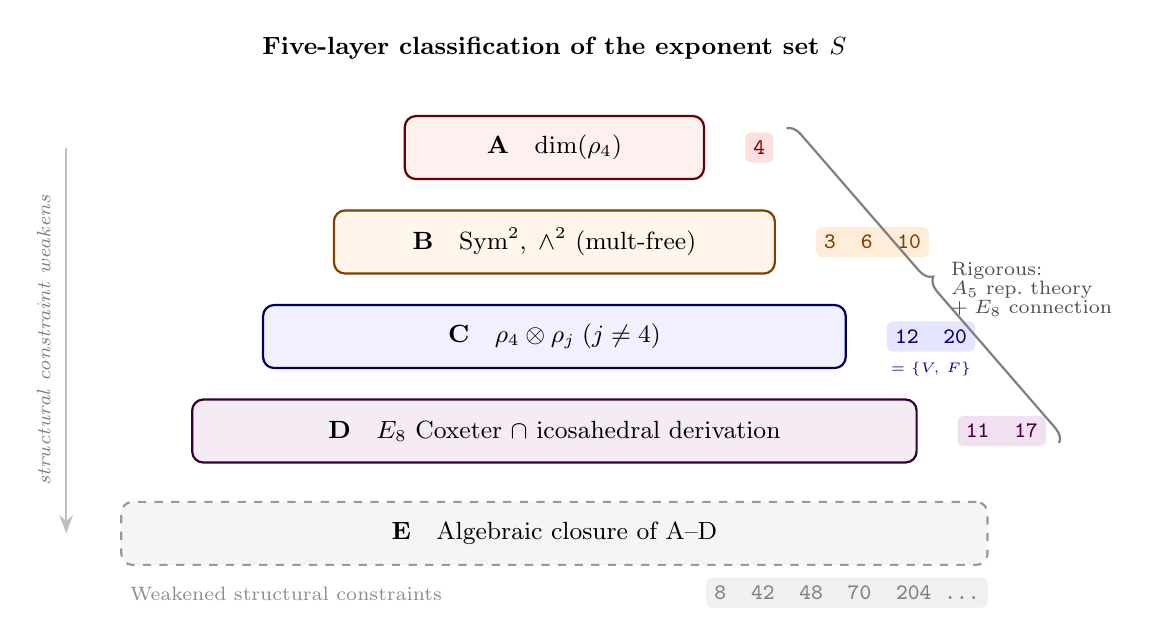
\begin{tikzpicture}[
  >=Stealth,
  layer/.style={
    draw, rounded corners=4pt, minimum height=0.8cm,
    font=\small, inner sep=6pt, align=center,
    line width=0.8pt
  },
  layerA/.style={layer, fill=red!6, draw=red!40!black},
  layerB/.style={layer, fill=orange!8, draw=orange!50!black},
  layerC/.style={layer, fill=blue!6, draw=blue!40!black},
  layerD/.style={layer, fill=violet!8, draw=violet!40!black},
  layerE/.style={layer, fill=black!4, draw=black!40, dashed},
  idxbox/.style={
    rounded corners=2pt, inner sep=3pt,
    font=\footnotesize\bfseries\ttfamily
  },
  brace/.style={decorate, decoration={brace, amplitude=5pt, raise=2pt},
    thick, draw=black!50},
]

%%% Center at x=0

%%% Title
\node[font=\small\bfseries, anchor=south] at (0,5.2)
  {Five-layer classification of the exponent set $S$};

%%% Downward arrow on far left
\draw[->, thick, gray!50]
  (-6.2,4.2) -- (-6.2,-0.7)
  node[midway, left=2pt, font=\scriptsize\itshape, text=black!50,
       rotate=90, anchor=south]
  {structural constraint weakens};

%%% Layer A
\node[layerA, minimum width=3.8cm] (LA) at (0,4.2)
  {\textbf{A}\quad $\dim(\rho_4)$};
\node[idxbox, fill=red!12, right=0.5cm of LA] (idxA)
  {\color{red!50!black}4};

%%% Layer B
\node[layerB, minimum width=5.6cm] (LB) at (0,3.0)
  {\textbf{B}\quad $\mathrm{Sym}^2,\;\wedge^2$ (mult-free)};
\node[idxbox, fill=orange!15, right=0.5cm of LB] (idxB)
  {\color{orange!50!black}3\;\; 6\;\; 10};

%%% Layer C
\node[layerC, minimum width=7.4cm] (LC) at (0,1.8)
  {\textbf{C}\quad $\rho_4 \otimes \rho_j\;(j\neq 4)$};
\node[idxbox, fill=blue!10, right=0.5cm of LC] (idxC)
  {\color{blue!50!black}12\;\; 20};
\node[font=\tiny, color=blue!60!black, below=0pt of idxC]
  {$= \{V,\, F\}$};

%%% Layer D
\node[layerD, minimum width=9.2cm] (LD) at (0,0.6)
  {\textbf{D}\quad $E_8$ Coxeter $\cap$ icosahedral derivation};
\node[idxbox, fill=violet!12, right=0.5cm of LD] (idxD)
  {\color{violet!50!black}11\;\; 17};

%%% Layer E (widest) --- indices below-right to avoid overflow
\node[layerE, minimum width=11.0cm] (LE) at (0,-0.7)
  {\textbf{E}\quad Algebraic closure of A--D};
\node[idxbox, fill=black!6, anchor=north east] (idxE)
  at ([yshift=-4pt]LE.south east)
  {\color{black!50}8\;\; 42\;\; 48\;\; 70\;\; 204\;\;\ldots};
\node[font=\scriptsize, text=black!45, anchor=north west]
  at ([yshift=-4pt]LE.south west)
  {Weakened structural constraints};

%%% Right brace: Layers A--D rigorous
\draw[brace] ([xshift=3pt]idxA.north east) -- ([xshift=3pt]idxD.south east)
  node[midway, right=8pt, font=\scriptsize, align=left, text=black!70]
  {Rigorous:\\[-1pt]$A_5$ rep.\ theory\\[-1pt]$+\; E_8$ connection};

\end{tikzpicture}
\caption{Five-layer classification of the exponent set $S$.
  Width represents the strength of the structural constraint:
  Layer~A (narrowest) is derived directly from the dimension of $\rho_4$,
  while Layer~E (widest, dashed) consists of algebraic compositions with
  gradually weakened constraints.
  Layers A--D are rigorously derived from $A_5$ representation theory
  and the $E_8$ connection; Layer~E extends through multiplicative
  and additive closure}\label{fig:five-layers}
\end{figure}


\subsection{\texorpdfstring{$E_8$}{E8} connection and dual membership filter
(P3)}\label{sec:P3}

Lifting to $\mathrm{Spin}(3) \cong \mathrm{SU}(2)$ gives the binary
icosahedral group $2I$ of order~120, the double cover of $A_5$. By the McKay
correspondence (1980)~\cite{McKay80}, $2I$ corresponds uniquely to the
affine $E_8$ Dynkin diagram.

\medskip
\noindent\textbf{Layer~D structure.}
Of the Coxeter exponents $\{1, 7, 11, 13, 17, 19, 23, 29\}$ of $E_8$, only
$\{11, 17\}$ can be independently derived as known physical combinations of
icosahedral parameters.

\begin{table}[ht]
\caption{Dual membership: both $E_8$ Coxeter exponents and independent
icosahedral combinations.}\label{tab:dual-membership}
\centering
\begin{tabular}{@{}lll@{}}
\toprule
$E_8$ exponent & Icosahedral derivation & Physical quantity \\
\midrule
$11$ & $\beta_0 = E/n + \chi/2 = V - 1$
  & $m_\mu/m_e \approx \varphi^{11}$ \\
$17$ & $F - n = 20 - 3$
  & $m_\tau/m_e \approx \varphi^{17}$ \\
\bottomrule
\end{tabular}
\end{table}

This dual membership---being both an $E_8$ Coxeter exponent and an
independent icosahedral combination---distinguishes $\{11, 17\}$ from all
other $E_8$ exponents.

\medskip
\noindent\textbf{Numerical necessity of the McKay correspondence.}
The Coxeter number $h(E_8) = 30 = E$ is a direct consequence of the McKay
correspondence and ensures that the appearance of $E_8$ is inseparable from
the icosahedral structure ($\sum m_i = 30$, $\sum m_i^2 = 120 = |2I|$). A
candidate path from $E_8$ to the SM ($E_8 \supset E_6 \supset
\mathrm{SU}(3)^3$) is an open problem in G1$'$ (emergence problem). Details
of the McKay correspondence, the representation theory of $2I$, and a
comparison with Lisi are given in Appendix~C.


\subsection{Summary of prohibited indices and falsification protocol}%
\label{sec:forbidden-summary}

\begin{table}[ht]
\caption{Prohibited indices and their exclusion mechanisms. Each prohibition
traces to one or more of (P1)--(P3).}\label{tab:prohibited}
\centering
\begin{tabular}{@{}clp{6.5cm}@{}}
\toprule
Prohibited index & Mechanism & Algebraic reason \\
\midrule
$9$  & (P1)
  & $\rho_4$-free: only solvable components from $\mathrm{SO}(3)$ \\
$15$ & (P1)+(P2)
  & $\rho_4$ absent; $\mathrm{Sym}^2\rho_5$ has multiplicity $> 1$ \\
$16$ & (P1)
  & $\rho_4 \otimes \rho_4$ (self-product): includes all 5 irreducibles,
    hence no selectivity \\
$25$ & (P1)
  & $\rho_4$ absent and self-product \\
\bottomrule
\end{tabular}
\end{table}

\begin{figure}[ht]
\centering
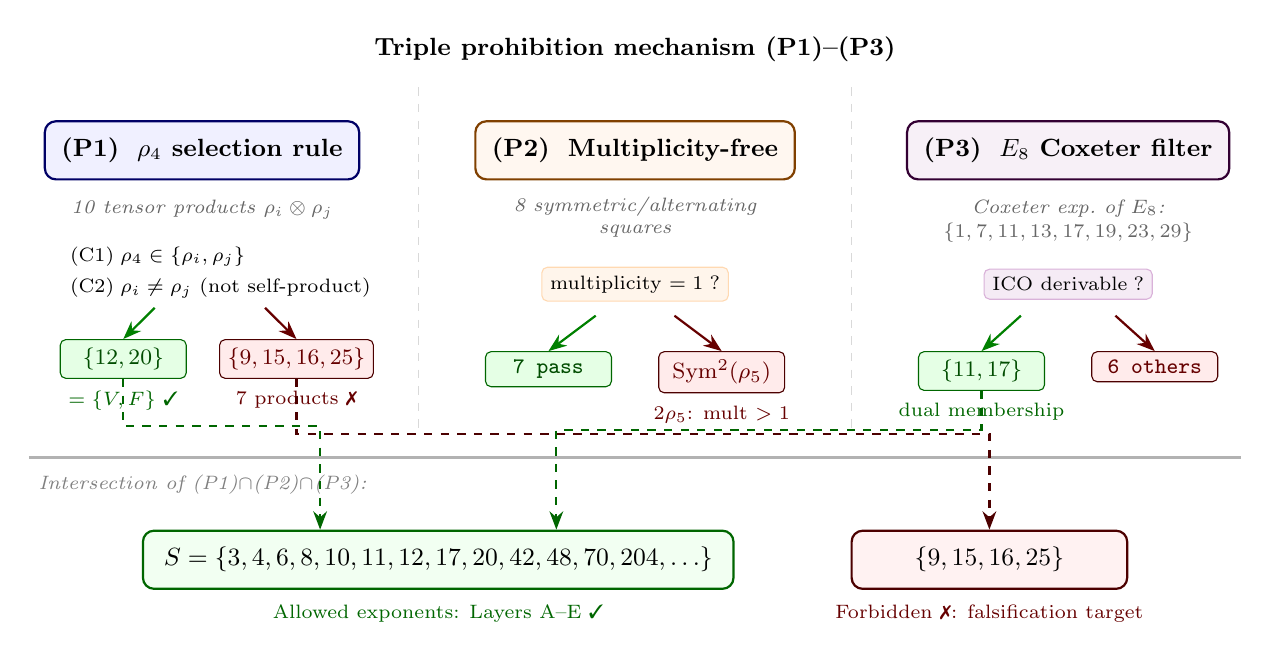
\begin{tikzpicture}[
  >=Stealth,
  node distance=0.5cm,
  tprod/.style={
    font=\footnotesize\ttfamily, minimum width=1.6cm,
    inner sep=3pt, align=center
  },
  allowed/.style={tprod, fill=green!10, draw=green!40!black,
    rounded corners=2pt, text=green!30!black},
  forbidden/.style={tprod, fill=red!8, draw=red!30!black,
    rounded corners=2pt, text=red!40!black},
  mech/.style={
    draw, thick, rounded corners=4pt, inner sep=6pt,
    font=\small\bfseries, minimum width=3.2cm, minimum height=0.7cm,
    align=center
  },
  filtarrow/.style={->, thick, color=black!50},
]

%%% Column centers: P1=0, P2=5.5, P3=11.0

%%% Title
\node[font=\small\bfseries, anchor=south] at (5.5,7.4)
  {Triple prohibition mechanism (P1)--(P3)};

%%% ===== P1: rho_4 selection rule (left column, center=0) =====
\node[mech, fill=blue!6, draw=blue!40!black] (P1) at (0,6.4)
  {(P1)\; $\rho_4$ selection rule};

\node[font=\scriptsize\itshape, color=black!60] at (0,5.65)
  {10 tensor products $\rho_i \otimes \rho_j$};

\node[font=\scriptsize, anchor=west] at (-1.8,5.05)
  {(C1)\;$\rho_4 \in \{\rho_i, \rho_j\}$};
\node[font=\scriptsize, anchor=west] at (-1.8,4.65)
  {(C2)\;$\rho_i \neq \rho_j$ (not self-product)};

\node[allowed] (alw) at (-1.0,3.75) {$\{12, 20\}$};
\node[font=\scriptsize, below=1pt of alw, text=green!40!black]
  {$=\{V, F\}$ \ding{51}};
\node[forbidden] (forb1) at (1.2,3.75) {$\{9,15,16,25\}$};
\node[font=\scriptsize, below=1pt of forb1, text=red!40!black]
  {7 products \ding{55}};
\draw[filtarrow, green!50!black] (-0.6,4.4) -- (alw.north);
\draw[filtarrow, red!40!black]  (0.8,4.4) -- (forb1.north);

%%% ===== P2: Multiplicity-free condition (center column, center=5.5) =====
\node[mech, fill=orange!6, draw=orange!50!black] (P2) at (5.5,6.4)
  {(P2)\; Multiplicity-free};

\node[font=\scriptsize\itshape, color=black!60, text width=3.2cm,
      align=center] at (5.5,5.55)
  {8 symmetric/alternating\\squares};

\node[font=\scriptsize, fill=orange!8, draw=orange!30, rounded corners=2pt,
      inner sep=3pt] (mfree) at (5.5,4.7)
  {multiplicity $= 1$\;?};

\node[allowed, anchor=north] (mfY) at (4.4,3.85) {7 pass};
\node[forbidden, anchor=north] (mfN) at (6.6,3.85)
  {$\mathrm{Sym}^2(\rho_5)$};
\node[font=\scriptsize, below=1pt of mfN, text=red!40!black]
  {$2\rho_5$: mult $> 1$};

\draw[filtarrow, green!50!black] (5.0,4.3) -- (mfY.north);
\draw[filtarrow, red!40!black] (6.0,4.3) -- (mfN.north);

%%% ===== P3: E8 Coxeter filter (right column, center=11.0) =====
\node[mech, fill=violet!6, draw=violet!40!black] (P3) at (11.0,6.4)
  {(P3)\; $E_8$ Coxeter filter};

\node[font=\scriptsize\itshape, color=black!60, text width=3.4cm,
      align=center] at (11.0,5.5)
  {Coxeter exp.\ of $E_8$:\\[1pt]$\{1,7,11,13,17,19,23,29\}$};

\node[font=\scriptsize, fill=violet!8, draw=violet!30, rounded corners=2pt,
      inner sep=3pt] (efilt) at (11.0,4.7)
  {ICO derivable\;?};

\node[allowed, anchor=north] (efY) at (9.9,3.85) {$\{11, 17\}$};
\node[font=\scriptsize, below=1pt of efY, text=green!40!black]
  {dual membership};
\node[forbidden, anchor=north] (efN) at (12.1,3.85) {6 others};

\draw[filtarrow, green!50!black] (10.4,4.3) -- (efY.north);
\draw[filtarrow, red!40!black] (11.6,4.3) -- (efN.north);

%%% Column separators
\draw[thin, black!15, dashed] (2.75,7.2) -- (2.75,2.8);
\draw[thin, black!15, dashed] (8.25,7.2) -- (8.25,2.8);

%%% ===== Bottom: Intersection yields S (moved down for clearance) =====
\draw[thick, black!30] (-2.2,2.5) -- (13.2,2.5);
\node[font=\scriptsize\itshape, color=black!50, anchor=west] at (-2.2,2.15)
  {Intersection of (P1)$\cap$(P2)$\cap$(P3):};

%%% Allowed set S
\node[draw, thick, rounded corners=4pt, fill=green!5,
      draw=green!40!black, inner sep=6pt,
      font=\small, minimum width=7.5cm] (setS) at (3.0,1.2)
  {$S = \{3, 4, 6, 8, 10, 11, 12, 17, 20, 42, 48, 70,
    204, \ldots\}$};
\node[font=\scriptsize, below=2pt of setS, text=green!40!black]
  {Allowed exponents: Layers A--E \ding{51}};

%%% Forbidden set
\node[draw, thick, rounded corners=4pt, fill=red!5,
      draw=red!30!black, inner sep=6pt,
      font=\small, minimum width=3.5cm] (forbset) at (10.0,1.2)
  {$\{9, 15, 16, 25\}$};
\node[font=\scriptsize, below=2pt of forbset, text=red!40!black]
  {Forbidden \ding{55}: falsification target};

%%% Dashed arrows from filters to bottom
\draw[->, thick, green!40!black, dashed]
  (alw.south) -- ++(0,-0.6) -| ([xshift=-1.5cm]setS.north);
\draw[->, thick, green!40!black, dashed]
  (efY.south) -- ++(0,-0.5) -| ([xshift=1.5cm]setS.north);
\draw[->, thick, red!30!black, dashed]
  (forb1.south) -- ++(0,-0.7) -| (forbset.north);

\end{tikzpicture}
\caption{Triple prohibition mechanism (P1)--(P3) and its role as a
  falsification target. The $\rho_4$ selection rule (P1) filters tensor
  products by requiring $\rho_4$ involvement in non-self-products;
  the multiplicity-free condition (P2) excludes $\mathrm{Sym}^2(\rho_5)$;
  the $E_8$ Coxeter filter (P3) retains only dual-membership exponents
  $\{11, 17\}$.
  The intersection defines the allowed exponent set $S$, while
  the forbidden indices $\{9, 15, 16, 25\}$ serve as pre-registered
  falsification targets}\label{fig:prohibition}
\end{figure}

\noindent\textbf{Falsification protocol.}
The system is rejected if a dimensionless ratio $R$ corresponding stably to a
forbidden index $p \in \{9, 15, 16, 25\}$ establishes
$|R/\varphi^p - 1| < 1\%$, or if the 10/10 agreement of the $\rho_4$
selection rule breaks down with the discovery of new structures.


\subsection{Breakdown of prohibition structures in alternative groups}%
\label{sec:alt-breakdown}

The prohibition structure (P1)--(P3) is unique to $A_5$ and does not hold for
other Klein candidates. $A_4$ (four irreducible representations, dimensions
$\{1, 1, 1, 3\}$) has only one tensor product and the selection rule
degenerates, while $S_4$ (five irreducible representations, dimensions
$\{1, 1, 2, 3, 3\}$) lacks a non-$\mathrm{SO}(3)$-derived irreducible
representation, and the premise of (P1) disappears. Neither group has
$\varphi$ in its character values. Only $A_5$ simultaneously satisfies
(a) five irreducible representations, (b) a non-$\mathrm{SO}(3)$-derived
$\rho_4$, and (c) character value $\varphi$.


\subsection{Representative numerical proximity (selection) and reference to
Appendix~A}\label{sec:numerical-proximity}

While this section argues for a prohibition structure, it would be incomplete
to entirely omit the correspondence with observations. Below, we present only
representative examples, primarily Type~I (RG-independent); a complete list of
approximately 46 entries is included in the protocolized observation log in
Appendix~A.

\begin{table}[ht]
\caption{Representative numerical proximity (selected). The Type column
corresponds to the RG survival classification in
Sect.~\ref{sec:scale-problem}.}\label{tab:representative}
\centering
\small
\begin{tabular*}{\textwidth}{@{\extracolsep{\fill}}clllcll@{}}
\toprule
\# & Quantity & ICO formula & ICO value & Exp.\ & Dev.\ & Type \\
\midrule
1 & $\alpha^{-1}$
  & $F\varphi^4$ & 137.08 & 137.036 & 0.034\% & I/III \\
2 & $\alpha_s(M_Z)$
  & $\mathrm{gap}/2$ & 0.1180 & 0.1180(9) & 0.03\% & I/III \\
3 & $\beta_0\,(n_f{=}0)$
  & $E/n + \chi/2$ & 11 & 11 & exact & I \\
4 & $m_\mu/m_e$
  & $\varphi^{11}$ & 199.0 & 206.8 & 3.8\% & II \\
5 & $m_\tau/m_e$
  & $\varphi^{17}$ & 3571 & 3477 & 2.7\% & II \\
6 & $m_t/m_b$
  & $E + V = 42$ & 42 & 41.5 & 1.2\% & I \\
7 & $\Omega_{\mathrm{DM}}/\Omega_b$
  & $|A_5|/V$ & 5.0 & 5.3(1) & ${\sim}\,6\%$ & II \\
\bottomrule
\end{tabular*}
\end{table}

\noindent\textbf{Notes.}
\#1 and \#2 share a closure relation, joining at
$\alpha_s \cdot \alpha^{-1} = 10\varphi$ (the triple lock value). The
exponents $\{11, 17\}$ of \#4 and \#5 are the $E_8$ dual assignments in
Sect.~\ref{sec:P3}. The systematic increase in deviation from Type~I (exact to
$0.03\%$) to Type~II ($2$--$6\%$) is consistent with the mechanism
classification in Sect.~\ref{sec:scale-problem}.

\medskip
\noindent\textbf{Limitations.}
(a) The correspondence rule (C1) has not been derived from first principles
(G3). (b) The ICO values are not aligned to a single scale (G2,
Sect.~\ref{sec:scale-problem}). (c) $\sin^2\theta_W \approx \mathrm{gap} =
2\alpha_s$, so these are not independent. There is no correspondence to the CP
phase.


\subsection{Epistemological summary of this section and terms of use for
Appendix~A}\label{sec:sec6-summary}

The argument in Sect.~\ref{sec:prohibition} is limited to two points:
\begin{enumerate}[nosep,label=(\roman*)]
  \item The representation theory of $A_5$ provides a closed description
    system for $\varphi$-power exponents, and there are non-trivial selection
    rules and a hierarchy (an algebraic fact).
  \item This system has a falsifiable prohibition structure
    (P1)--(P3) (pre-registered falsification conditions).
\end{enumerate}

The dynamical mechanism (G4), the derivation of the correspondence rule (G3),
and the scale problem (G2) are explicit non-assertions.

\medskip
\noindent\textbf{Appendix~A operating terms.}
Appendix~A complements the logical core of the main text ($A_5$ uniqueness,
prohibition structures, and Type~I proof of concept) as an audit log, not as
the core of the evidence. To prevent reactive responses and double counting,
all items are assigned a protocol (R1)--(R3): Role (Input~I / Selection~S /
Prediction~P / Derivation~D / Exploration~X / Tension~T), Type (I/II/III),
and Forb (prohibition index check). Items used for selection are not counted
as successes, and prohibition index violations are kept as negative controls
(see A.12). Numerical proximity is not used in the inference of $A_5$ (the
inference direction is reversed), and the falsifiable content of the system is
encoded in the prohibition/permission structure.

%% ============================================================
%% SECTION 7: Limitations, Prior Work, and Open Problems
%% ============================================================
\section{Limitations, Prior Work, and Open Problems}\label{sec:limitations}

In this section, we frankly list the limitations of this paper, briefly
highlight differences from previous research, and present open problems
G1$'$--G7 as a prioritized roadmap.


\subsection{What this paper does not claim (explicit listing of limitations)}%
\label{sec:not-claimed}

The following items are outside the scope of this paper and no claims are made.

\medskip
\noindent\textbf{(L1) Lack of dynamical mechanism.}
It is unclear how the algebraic structure of $A_5$ is translated into
observables. This paper provides ``algebraic constraints,'' not ``dynamics.''

\medskip
\noindent\textbf{(L2) Absence of external--internal gauge connection.}
$A_5$ holonomy is a constraint on the exterior space and does not directly
determine the interior gauge symmetry
$\mathrm{SU}(3) \times \mathrm{SU}(2) \times \mathrm{U}(1)$. The McKay path
($2I \to E_8 \to \mathrm{SU}(3)^3$) only indicates the existence of a
candidate path, but is not a dynamical derivation (G1$'$).

\medskip
\noindent\textbf{(L3) Non-derivability of correspondence rules.}
The correspondence rule (C1) (faces $\to$ electromagnetic, edges $\to$ strong
force, vertices $\to$ gravity) is not derived from first principles (G3). The
choice of (C1) among the $3! = 6$ possible assignments is a posteriori, and
the numerical table in Sect.~\ref{sec:numerical-proximity} cannot escape this
a posteriori status.

\medskip
\noindent\textbf{(L4) Scale issues.}
Although we decomposed the problem into three types (Type~I--III) in
Sect.~\ref{sec:scale-problem}, it is not yet clear which conservation mechanism is
physically realized (G2). All correspondences other than Type~I (integer
structural constants) remain hypotheses to be tested.

\medskip
\noindent\textbf{(L5) Dynamical basis of determinant scaling.}
In the derivation of
$\mathrm{gap} = \lambda_\varphi^{\dim(\rho_3)} = 1/\varphi^3$
(Sect.~\ref{sec:phi-derivation}), we established the uniqueness of
$\lambda_\varphi$, $\dim(\rho_3) = 3$, and that $\lambda_\varphi$ is a
representation-theoretic signature of the Galois exchange
($C_5 \leftrightarrow C_5^2$ via $g \mapsto g^2$). What remains unresolved is
the dynamical basis of determinant scaling (G5).

\medskip
\noindent\textbf{(L6) Absence of CP phase.}
$A_5$ has only real representations and does not naturally generate complex
phases. The structure corresponding to CP violation is beyond the scope of
this paper. Note that the reality of $\rho_3$ is also the
representation-theoretic basis for
$\chi_{\rho_3}(g^{-1}) = \chi_{\rho_3}(g)$ (inversion preserves conjugacy
classes; see Remark~\ref{rem:galois}\,(i)), and is inseparably related to the
Galois structure of L5.

\medskip
\noindent\textbf{(L7) Unformalized Klein classification.}
The only unformalized proposition in the argument chain. Once completed, the
entire argument will be machine-verifiable from end to end.


\subsection{Comparison with previous studies}\label{sec:comparison}

The geometric derivation of coupling constants has a long history. We briefly
highlight the methodological differences.

\medskip
\noindent\textbf{Wyler (1969).}
Derived $\alpha^{-1} \approx 137.036$ from the volume ratio of a symmetric
space, but there is no mathematical necessity for the choice of symmetric
space (Gilmore's criticism). In this paper, $A_5$ is uniquely determined by
elimination from the three principles.

\medskip
\noindent\textbf{Atiyah (2018).}
Attempted a derivation of $\alpha^{-1}$ using the $6j$ symbol, but the work
is incomplete. It shares the focus on $A_5$ representation theory, but differs
in that the reasons for choosing $A_5$ are explicitly discussed here.

\medskip
\noindent\textbf{Koide (1981).}
The empirical formula for charged lepton masses gives $Q = 2/3$. In this
paper, $m_\mu/m_e = \varphi^{11}$, $m_\tau/m_e = \varphi^{17}$,
$Q \approx 0.6655$ (deviation~$0.2\%$), and the formal equivalence to
$Q = 2/3 = 1 - 1/n$ suggests a connection with spatial dimensions.

\medskip
\noindent\textbf{Lisi (2007).}
Starts from $E_8$ as a direct assumption. In this paper, $E_8$ is a
consequence of the McKay correspondence and is not an assumption.
Distler--Garibaldi's criticism~\cite{DistlerGaribaldi09} does not directly apply to
the connection path in this paper (see Appendix~C.6 for details).

\medskip
\noindent\textbf{Differences from discrete quantum gravity approaches.}
Regge calculus, CDT, and spin foam all start with discretization as an
``approximation of a continuum theory,'' with physical constants input as
parameters of the action. Our approach reverses this logic: we treat finite
group holonomy as a fundamental entity, and the uniqueness established by the
three principles (Theorem~\ref{thm:main}) completely eliminates the degrees of
freedom of the discretization, allowing algebraic data to constrain the
physical constants. However, our approach is positioned as a complement to
discrete quantum gravity, not a replacement.

\medskip
\noindent\textbf{Novelty of this paper.}
The mathematical content itself is not new (the central result of
Sect.~\ref{sec:main-theorem} is a known contrapositive, and the algebra in
Sect.~\ref{sec:prohibition} is a standard fact of $A_5$ representation theory).
The novelty lies in the three-stage reconstruction: (N1) reformulation as a
physical principle (H3*), (N2) systematization of robustness through
multi-path convergence of the five conditions, and (N3) connection to the
prohibition structure (P1)--(P3). In the context of \emph{Foundations of
Physics}, the core contribution is the question itself: ``Why does a known
theorem reappear as a physical principle?''


\subsection{Open problems G1\texorpdfstring{$'$}{'}--G7: prioritized roadmap}%
\label{sec:open-problems}

\noindent\textbf{Research strategic priorities.}

\emph{Top priorities:} G2 (scale issues) and G6 (physical realization). G2 can
be systematically tackled through the three-type analysis in
Sect.~\ref{sec:scale-problem}, and influences the physical interpretation of the
entire system. G6 is the only problem that can be experimentally explored
independently of G1$'$.

\emph{Second priority:} G3 (correspondence) and G4 (index). The internal
consistency of the algebraic structure of $A_5$ can be explored independently
of G1$'$.

\emph{Core issues:} G1$'$ (emergence) and G5 (gap). The most fundamental but
also the most difficult.

\begin{table}[ht]
\caption{Open problems G1$'$--G7: prioritized research
roadmap.}\label{tab:roadmap}
\centering
\small
\begin{tabular*}{\textwidth}{@{\extracolsep{\fill}}cp{3.2cm}cp{5.5cm}@{}}
\toprule
Problem & Content & Priority & Strategy route \\
\midrule
G1$'$ & Emergence: dynamical derivation $A_5 \to$ SM
  & Core
  & McKay path $2I \to E_8 \to E_6 \to \mathrm{SU}(3)^3$ (L2 unsolved).
    String-theoretic candidates: $\mathbb{C}^2/2I$ ADE singularity~(I),
    heterotic $E_8 \times E_8$~(II) (Appendix~F, G7). \\
G2 & Scale issue: identifying RG survival mechanisms
  & Highest
  & Sect.~\ref{sec:scale-problem} Type~I--III analysis, lattice calculations \\
G3 & Correspondence: first-principles derivation of (C1)
  & 2nd
  & Structural correspondence between stabilizer orders $\{3,2,5\}$ and
    gauge rank \\
G4 & Index problem: dynamical basis of prohibition structures
  & 2nd
  & First-principles derivation of $\rho_4$ selection rule (G4$'$) \\
G5 & Determinant scaling: dynamical basis of
    $\lambda_\varphi^{\dim(\rho_3)}$
  & Core
  & Discrete holonomy $\leftrightarrow$ field theory connection (subproblem
    of G1$'$) \\
G6 & Physical realization: experimental search for solvable opacity
  & Highest
  & $A_5$ gauge theory anyons, interference experiments \\
G7 & String theory consistency: $2I \hookrightarrow E_8$ verification
  & 2nd
  & ADE singularities, heterotic embeddings, Dechant construction
    (Appendix~F) \\
\bottomrule
\end{tabular*}
\end{table}

\noindent\textbf{Formulation of each problem.}

\medskip
\noindent\textbf{G1$'$ (emergence problem).}
From the algebraic rigidity of $A_5$, construct a framework that directly
describes the segmentation of forces, the hierarchy of matter, and the scale
structure without free parameters. The gauge group of the SM is not a goal to
be achieved, but should be recovered a posteriori as a low-energy effective
description of the physics generated by $A_5$.

\medskip
\noindent\textbf{G2 (scale problem).}
See the three-type analysis in Sect.~\ref{sec:scale-problem}. Type~I is solved,
Type~II is theoretically explorable, and Type~III is observationally testable.

\medskip
\noindent\textbf{G3 (correspondence problem).}
First-principles derivation of the correspondence rule (C1). The structural
correspondence between the stabilizer group orders $\{3, 2, 5\}$ and the
gauge group rank, and the triple lock value
$10 = E/n = F/2 = |A_5|/6$ are key clues.

\medskip
\noindent\textbf{G4 (index problem).}
The dynamical basis of the prohibition structure in Sect.~\ref{sec:prohibition}. Why
specific physical quantities are assigned specific $\varphi$-power exponents.
The first-principles derivation of the $\rho_4$ selection rule is formulated
as sub-problem G4$'$.

\medskip
\noindent\textbf{G5 (determinant scaling problem).}
Dynamical basis for
$\lambda_\varphi^{\dim(\rho_3)} = 1/\varphi^3$ (see L5). It was established
in Sect.~\ref{sec:phi-derivation} that $\lambda_\varphi$ is a
representation-theoretic trace of the Galois exchange
$\sigma \colon \varphi \mapsto -1/\varphi$, realized group-theoretically by
$g \mapsto g^2$. What remains unresolved is the dynamical basis for why
$\lambda_\varphi$ raised to the $\dim(\rho_3)$ power controls the physical
coupling parameters. Candidate approaches: (i) spectral analysis of the
$\rho_3$ determinant in the plaquette action of discrete gauge theories,
(ii) saddle-point approximation of the partition function in the $A_5$ version
of Dijkgraaf--Witten theory~\cite{DijkgraafWitten90}. This is a subproblem of G1$'$.

\medskip
\noindent\textbf{G6 (physical realization of solvable opacity).}
The most direct problem connecting the no-go theorem of
Sect.~\ref{sec:solvable-opacity} to experimental exploration: (i) anyons in $A_5$
gauge theory (non-solvable phases in discrete gauge theories), and (ii) quantum
computation tasks specific to $A_5$ (interference experiments on phase factors
that do not appear in solvable groups).

\medskip
\noindent\textbf{G7 (string theory integration).}
Consistency checks of the $A_5 \to 2I \to E_8$ chain with the standard $E_8$
construction of superstring theory. (G7a) Calculation of the
$2I \hookrightarrow E_8$ centralizer group. (G7b) Compactification
interpretation of forbidden indices. (G7c) Connection between Dechant's
$3 \to 8$ dimensionality increase and critical dimensions. Details are given
in Appendix~F.

\medskip
\noindent\textbf{Interrelationships of open problems.}
The development of G1$'$ naturally subsumes G3, but G3 and G4 can be explored
independently of G1$'$ as problems on the algebraic internal structure of
$A_5$. The solution of G2 directly affects the interpretation of G4 and G5.
G6 can be explored independently of G1$'$ and is the problem closest to
experiment, based on Sect.~\ref{sec:solvable-opacity}.


\subsection{Information barriers and entropy (preview)}\label{sec:entropy-preview}

The solvable opacity in Sect.~\ref{sec:solvable-opacity} shows that the 60
elements of $A_5$ cannot be distinguished by solvable probes, generating an
exponential information barrier of $60^N \geq 2^{5N}$ in $N$ steps. This
suggests: (i) a group-theoretic reinterpretation of the Boltzmann entropy (an
algebraic basis for coarse-graining), (ii) an algebraic basis for
irreversibility (a solvable-group universe has zero information barrier), and
(iii) a formal connection to the cosmological constant
($\Lambda \ell_{\mathrm{Pl}}^2 \sim \varphi^{-600}$,
$600 = 2 \times 291 + (E - V)$). All of these are speculative interpretations
(Layer~P/E), and details are provided in Appendix~D.

%% ============================================================
%% SECTION 8: Conclusion
%% ============================================================
\section{Conclusion}\label{sec:conclusion}

\subsection{Summary of key findings}\label{sec:summary}

This paper proves that the holonomy group $A_5$ is uniquely selected under the
three principles (H1)--(H3) (Theorem~\ref{thm:main}, robust due to the
convergence of five conditions, Lean~4 formally verified), and obtains the
following consequences.

\begin{enumerate}[nosep,label=(\roman*)]
  \item \textbf{Proof of concept (Sect.~\ref{sec:beta0}).}
    $\beta_0^{\ICO} = E/n + \chi/2 = V - 1 = 11$ (identity).
  \item \textbf{Prohibition structure (Sect.~\ref{sec:prohibition}).}
    Pre-registration of the forbidden exponents $\{9, 15, 16, 25\}$ by
    (P1)--(P3).
  \item \textbf{Decomposition of the scaling problem
    (Sect.~\ref{sec:scale-problem}).}
    Type~I--III classification. The main text focuses on Type~I.
\end{enumerate}


\subsection{The structure of conditional consequences}%
\label{sec:conditional-structure}

The focus of this paper is not to assert that ``$A_5$ is true,'' but to list
the necessary conditions for a $\varphi$-power system to hold as three layers,
and to provide independent falsification conditions for each layer.

\medskip
\noindent\textbf{Layer~1 (Existence conditions).}
$\varphi$ does not appear if any of three-dimensionality, non-solvability,
irreducibility, or the perfect group property is missing
(Theorem~\ref{thm:main}).

\medskip
\noindent\textbf{Layer~2 (Structural conditions).}
The $\rho_4$ selection rule, the multiplicity-free condition, and the $E_8$
Coxeter-exponent filter form the prohibition structure.

\medskip
\noindent\textbf{Layer~3 (Consistency conditions).}
Micro and macro are connected by inter-sector consistency relations such as
$\beta_0 = V - 1 = 11$.

\medskip
Each layer can be independently falsified.

\medskip
\noindent\textbf{Five Cosmic Constraints.}
The above three layers are unified into five constraints: (CC1) information
barrier, (CC2) symmetry segmentation, (CC3) prohibition structure, (CC4)
necessity of scale hierarchy, and (CC5) cosmological consistency, based on the
single algebraic fact that $A_5$ is the smallest non-solvable finite simple
group (Appendix~E).


\subsection{What is established and what remains unresolved}%
\label{sec:established}

\begin{table}[ht]
\caption{Established results (top) and unresolved problems
(bottom).}\label{tab:established}
\centering
\small
\begin{tabular}{@{}p{5.8cm}p{5.8cm}@{}}
\toprule
Established result & Epistemic status \\
\midrule
$A_5$ uniqueness (Theorem~\ref{thm:main},
  Corollaries~\ref{cor:solvable-opacity}--\ref{cor:fivefold})
  & Layer~M (formally verified) \\
Solvable opacity (Theorem~\ref{thm:opacity},
  Corollaries~\ref{cor:degeneracy}--\ref{cor:cumulative})
  & Layer~M (formally verified) \\
Algebraic facts of the prohibition structure (P1)--(P3)
  & Layer~M (derived from character table and tensor products) \\
$\beta_0 = V - 1 \equiv E/n + \chi/2 = 11$
  & Layer~M (identity, formally verified) \\
\midrule
Unresolved problem & Reference \\
\midrule
Dynamical mechanism ($A_5 \to$ observables)
  & G1$'$ (Sect.~\ref{sec:open-problems}) \\
Scale issue (identifying RG survival mechanisms)
  & G2 (Sect.~\ref{sec:scale-problem}, Sect.~\ref{sec:open-problems}) \\
Deriving the correspondence rules
  & G3 (Sect.~\ref{sec:open-problems}) \\
Dynamical basis of the prohibition structure
  & G4 (Sect.~\ref{sec:open-problems}) \\
Dynamical basis of determinant scaling
  & G5 (Sect.~\ref{sec:open-problems}) \\
Experimental verification of solvable opacity
  & G6 (Sect.~\ref{sec:open-problems}) \\
\bottomrule
\end{tabular}
\end{table}


\subsection{Outlook}\label{sec:outlook}

The core questions boil down to two: why (H1)(H2)(H3) are physically
plausible, and by what mechanism the discrete structure of $A_5$ is translated
into observables. For the former, $\beta_0 = 11$
(Sect.~\ref{sec:reconstruction}) provides a posteriori support, and the
prohibition structure (Sect.~\ref{sec:prohibition}) provides falsifiability. For
the latter, a research program is formulated as G1$'$--G7.

The mathematical chain $A_5 \to 2I \to E_8$ is structurally consistent with
standard constructions of superstring theory (Appendix~F). Why the algebraic
rigidity of $A_5$---the smallest non-solvable finite simple group---resonates
with so many physical structures is a question beyond the scope of this paper.
This paper provides a rigorous starting point for exploring that question: a
set of formally verified theorems, a pre-registered list of falsification
conditions, and prioritized open problems.


%% ============================================================
%% Acknowledgments + Declarations (Springer Nature mandatory)
%% ============================================================
\backmatter

\bmhead{Acknowledgments}

The formal verification in this paper is based on the Lean~4
theorem prover~\cite{Lean4} and the Mathlib mathematical
library~\cite{Mathlib}.
The author thanks the developer communities of both projects.

\bmhead{Statements and Declarations}

\paragraph{Funding.}
This research received no external funding.

\paragraph{Competing interests.}
The author declares no competing interests.

\paragraph{Ethics approval and consent to participate.}
Not applicable.

\paragraph{Consent for publication.}
Not applicable.

\paragraph{Data availability.}
This paper contains no experimental data.
All numerical values of physical constants referenced in this work
are taken from published sources cited in the bibliography.

\paragraph{Materials availability.}
Not applicable.

\paragraph{Code availability.}
The complete Lean~4 source code for the formal verification
(sorry\,$=$\,0, axiom\,$=$\,0) and the theorem--identifier
correspondence table are publicly available at
\url{https://github.com/nuu/A5CosmicNecessity}
and permanently archived at Zenodo
(\url{https://doi.org/10.5281/zenodo.18801089})
under the Apache License 2.0.
The repository includes all files necessary to reproduce
the verification: \texttt{lakefile.lean}, Mathlib dependency
specifications, and per-section Lean source files
(\texttt{Section1\_Introduction.lean} through
\texttt{Section8\_Conclusion.lean} and auxiliary modules).

\paragraph{Author contribution.}
M.~Numagaki is the sole author and is responsible for the
conception of the theoretical framework,
all mathematical proofs and their Lean~4 formalization,
the numerical analysis, and the writing of the manuscript.

\paragraph{Use of AI-assisted tools.}
Use of Generative AI and AI-assisted technologies in the writing process
During the preparation of this work the author used ChatGPT in order to improve the readability and language of the manuscript. After using this tool/service, the author reviewed and edited the content as needed and takes full responsibility for the content of the publication.


%% ============================================================
%% APPENDIX A: Protocolized Observation Log
%% ============================================================
\begin{appendices}

%%% Appendix numbering: Table A.1, Eq. (A.1), etc.
\numberwithin{table}{section}
\numberwithin{equation}{section}

\section{Protocolized Observation Log}\label{app:observation}

A complete list (46 items) of correspondences between ICO formulas and
physical constants constructed from the discrete algebraic structure of $A_5$.
This appendix follows the terms of use in Sect.~\ref{sec:sec6-summary} and
complements the logical core of the main text ($A_5$ uniqueness, prohibition
structure, Type~I proof of concept). It is operated as an audit log.


\subsection{Protocol definitions (R1)--(R3)}\label{app:protocol}

To prevent retroactive counting and double counting, all 46 items are assigned
the following three protocol columns.

\medskip
\noindent\textbf{(R1) Role.}
Each item is classified into six categories to structurally prevent inflation
of ``success rates.''

\begin{table}[ht]
\caption{(R1) Role classification.}\label{tab:R1}
\centering
\small
\begin{tabular}{@{}llp{6cm}@{}}
\toprule
Role & Meaning & Constraint \\
\midrule
I & Input (fixed)
  & Cannot be included in success rate or prediction count \\
S & Selection set (used to calibrate C1)
  & Cannot be included in success rate or prediction count \\
P & Predictive holdout
  & Candidates that the text can reference as ``achievements'' \\
D & Derived (depends on other items)
  & Cannot be counted as an independent prediction.
    Dependency noted in Dep column. \\
X & Exploratory (uncertain/undetermined)
  & Immature. Promote to P or reject in the future. \\
T & Tension / negative control
  & Retained as a failure example. Negative control for the
    prohibition structure. \\
\bottomrule
\end{tabular}
\end{table}

\noindent\textbf{(R2) Type (RG survival category).}
Each item's preservation mechanism under RG flow is classified according to
the three types of Sect.~\ref{sec:scale-problem}.

\begin{table}[ht]
\caption{(R2) RG survival type.}\label{tab:R2}
\centering
\begin{tabular}{@{}lll@{}}
\toprule
Type & Meaning & Main-text status \\
\midrule
I   & RG-independent (integer/topological)
    & Subject of main-text strong argument \\
II  & Fixed point / universal quantity hypothesis
    & Downgraded to test hypothesis \\
III & Cosmic freeze-out / scale dependence
    & Downgraded to observation programme \\
\bottomrule
\end{tabular}
\end{table}

\noindent\textbf{(R3) Forb (prohibition index check).}
Match against the forbidden set $\{9, 15, 16, 25\}$ of
Sect.~\ref{sec:forbidden-summary}. Items falling within the forbidden index are
isolated as T (negative control) and excluded from the allowed set
$S_{\mathrm{allowed}}$.

\medskip
\noindent\textbf{Input summary.}
From $n = 3$ (spatial dimension) and $A_5$ (Theorem~\ref{thm:main}):
$(F, E, V) = (20, 30, 12)$, $\varphi = (1+\sqrt{5})/2$, $|A_5| = 60$,
$\chi = 2$, $\mathrm{gap} = 1/\varphi^3$. The single dimensional input is
$M_Z = 91.19$~GeV.

\medskip
\noindent\textbf{Legend.}
Deviation $= |(\mathrm{ICO} - \mathrm{obs})/\mathrm{obs}|$.
$\varphi$-exp $=$ $\varphi$ exponent.
Ly $=$ five-layer classification (A--E) from Sect.~\ref{sec:P2}.
Forb: \ding{51} $=$ allowed, $\triangle$ $=$ falls in forbidden set,
--- $=$ no exponent.
Dep: --- $=$ independent, $\nearrow$\# $=$ depends on item \#.


\subsection{Gauge coupling constants and scales}\label{app:gauge}

\begin{table}[ht]
\caption{Gauge coupling constants and scales (\#1--\#10).}\label{tab:app-gauge}
\centering
\scriptsize
\setlength{\tabcolsep}{3pt}
\begin{tabular*}{\textwidth}{@{\extracolsep{\fill}}clllccccccl@{}}
\toprule
\# & Quantity & ICO formula & ICO & Exp.\ & Dev.\ & $\varphi$-e & Ly & R & Ty
  & Dep \\
\midrule
1  & $\alpha^{-1}$   & $F\varphi^4$    & 137.08  & 137.036  & 0.034\%
   & 4   & A & S  & II  & --- \\
2  & $\alpha_s(M_Z)$ & $\mathrm{gap}/2$& 0.1180  & 0.1180   & 0.03\%
   & 3   & B & S  & II  & --- \\
3  & $\sin^2\theta_W$& $\mathrm{gap}(1{-}1/(F\pi))$ & 0.2312 & 0.2312
   & 0.4\% & 3 & B & P & II & --- \\
4  & $\alpha/\alpha_G$& $\varphi^{204}$ & ${\sim}10^{44}$ & ${\sim}10^{44}$
   & ${\sim}2\%$ & 204 & E & P & II & --- \\
5  & $\alpha_s/\alpha$& $10\varphi$     & 16.18   & 16.16    & ${<}0.1\%$
   & --- & --- & D & II & $\nearrow$1,2 \\
6  & $\beta_0(n_f{=}0)$& $E/n{+}\chi/2$& 11      & 11       & exact
   & --- & --- & P & I  & --- \\
7  & Quark coeff.\    & $|A_5|/(En)$    & $2/3$   & $2/3$    & exact
   & --- & --- & P & I  & --- \\
8  & $\Lambda_{\mathrm{QCD}}$& $M_Z/\varphi^{12}$ & 283~MeV & 292~MeV
   & 3.1\% & 12 & C & P & III & --- \\
9  & $M_{\mathrm{Pl}}/m_e$& $\sqrt{F}\,\varphi^{104}$
   & ${\sim}2.4{\times}10^{22}$ & ${\sim}2.4{\times}10^{22}$ & ${\sim}1.6\%$
   & 104 & E & D & III & $\nearrow$4 \\
10 & $M_{\mathrm{GUT}}/M_Z$& $\varphi^{68}$ & ${\sim}10^{14}$
   & ${\sim}10^{14}$ & order & 68 & E & D & III & $\nearrow$4 \\
\bottomrule
\end{tabular*}
\end{table}

\noindent\textbf{Note.}
\#1 and \#2 are used to select the correspondence rule (C1), so Role $=$ S.
\#5 is the ratio of \#1 and \#2 and is a derivative. \#6 and \#7 are
RG-independent integers/rationals (Type~I), and are the core of the proof of
concept in Sect.~\ref{sec:beta0}.


\subsection{Charged lepton masses}\label{app:leptons}

\begin{table}[ht]
\caption{Charged lepton masses (\#11--\#14).}\label{tab:app-lepton}
\centering
\scriptsize
\setlength{\tabcolsep}{3pt}
\begin{tabular*}{\textwidth}{@{\extracolsep{\fill}}clllccccccl@{}}
\toprule
\# & Quantity & ICO formula & ICO & Exp.\ & Dev.\ & $\varphi$-e & Ly & R & Ty
  & Dep \\
\midrule
11 & $m_e$       & $M_Z\alpha^2(1{-}\alpha)/(n\pi)$ & 0.511~MeV & 0.511~MeV
   & 0.2\% & --- & --- & D & II & $\nearrow$1,27 \\
12 & $m_\mu/m_e$ & $\varphi^{11}$ & 199.0 & 206.8 & 3.7\%
   & 11  & D & P & II & --- \\
13 & $m_\tau/m_e$& $\varphi^{17}$ & 3571  & 3477  & 2.7\%
   & 17  & D & P & II & --- \\
14 & Koide $Q$   & $1{-}1/n = 2/3$& 0.6667& 0.6666& 0.01\%
   & --- & --- & D & II & $\nearrow$12,13 \\
\bottomrule
\end{tabular*}
\end{table}

\noindent\textbf{Note.}
\#11 depends on \#1 ($\alpha$) and \#27 ($M_Z$), hence D. The exponents
$\{11, 17\}$ of \#12 and \#13 are the $E_8$ dual assignments (Layer~D) of
Sect.~\ref{sec:P3}. \#14 is a derived quantity depending on \#12 and \#13.


\subsection{Quark masses}\label{app:quarks}

\begin{table}[ht]
\caption{Quark masses (\#15--\#20).}\label{tab:app-quark}
\centering
\scriptsize
\setlength{\tabcolsep}{3pt}
\begin{tabular*}{\textwidth}{@{\extracolsep{\fill}}clllccccccl@{}}
\toprule
\# & Quantity & ICO formula & ICO & Exp.\ & Dev.\ & $\varphi$-e & Ly & R & Ty
  & Dep \\
\midrule
15 & $m_t$       & $M_Z\varphi^2/\sqrt{2}\cdots$ & 172.8~GeV & 172.6~GeV
   & 0.14\% & 2 & --- & P & II & --- \\
16 & $m_t/m_b$   & $F{+}V{+}E/n = 42$ & 42 & 41.5 & 1--2\%
   & 42  & E & P & II & --- \\
17 & $m_t/m_c$   & $\varphi^{10}$ & 123.0 & $134(\pm)$ & scheme
   & 10  & B & P & II & --- \\
18 & $m_c/m_s$   & $V{+}\varphi$ & 13.62 & $13.6(\pm)$ & ${\sim}0.2\%$
   & --- & --- & D & II & $\nearrow$17 \\
19 & $m_s/m_d$   & $F = 20$      & 20    & $20(\pm)$   & ${\sim}0.2\%$
   & 20  & C & D & II & $\nearrow$18 \\
20 & $m_d/m_u$   & $\sqrt{5}$    & 2.236 & $2.16(\pm)$ & ${\sim}3.5\%$
   & --- & --- & P & II & --- \\
\bottomrule
\end{tabular*}
\end{table}

\noindent\textbf{Note.}
Quark masses have large uncertainty due to scheme dependence. The ICO value of
\#16 is an integer (42), but the physical quantity $m_t/m_b$ itself is a pole
mass ratio with scheme dependence, so it is classified as Type~II.


\subsection{Neutrino masses (exploratory)}\label{app:neutrinos}

\begin{table}[ht]
\caption{Neutrino masses (\#21--\#23).}\label{tab:app-neutrino}
\centering
\scriptsize
\setlength{\tabcolsep}{3pt}
\begin{tabular*}{\textwidth}{@{\extracolsep{\fill}}clllccccccl@{}}
\toprule
\# & Quantity & ICO formula & ICO & Exp.\ & Dev.\ & $\varphi$-e & Ly & R & Ty
  & Dep \\
\midrule
21 & $m_{\nu_3}$ & $(m_e^2/M_Z)\varphi^{-8}$ & ${\sim}0.06$~eV
   & ${\sim}0.05$~eV & ${\sim}22\%$ & 8 & E & X & III & --- \\
22 & $m_{\nu_2}/m_{\nu_3}$ & $\varphi^{-6}$ & 0.056 & ${\sim}0.17$
   & $\times 3$ & 6 & B & X & III & --- \\
23 & $m_{\nu_1}/m_{\nu_2}$ & $\varphi^{-11}$ & 0.005 & upper lim.\
   & --- & 11 & D & X & III & $\nearrow$22 \\
\bottomrule
\end{tabular*}
\end{table}

\noindent\textbf{Note.}
Normal ordering assumed. Absolute mass is uncertain; Role $=$ X due to large
experimental uncertainty. Next-generation experiments such as DUNE can upgrade
or reject these entries.


\subsection{Mixing angles}\label{app:mixing}

\begin{table}[ht]
\caption{Mixing angles (\#24--\#26).}\label{tab:app-mixing}
\centering
\scriptsize
\setlength{\tabcolsep}{3pt}
\begin{tabular*}{\textwidth}{@{\extracolsep{\fill}}clllccccccl@{}}
\toprule
\# & Quantity & ICO formula & ICO & Exp.\ & Dev.\ & $\varphi$-e & Ly & R & Ty
  & Dep \\
\midrule
24 & $\sin\theta_C$       & gap     & 0.2361 & 0.2253   & 4.8\%
   & 3  & B & X & II & --- \\
25 & $\sin^2\theta_{13}(\nu)$ & $2/(5\varphi^6)$ & 0.0223 & 0.0218
   & 2.3\% & 6 & B & X & II & --- \\
26 & $|V_{ub}|$ suppression & $\mathrm{gap}^3$ & 0.013 & 0.004
   & $\times 3$ & 9 & --- & T & II & --- \\
\bottomrule
\end{tabular*}
\end{table}

\noindent\textbf{Note.}
\#26 is the only item for which $\varphi$-exp $= 9$ falls in the forbidden
set $\{9, 15, 16, 25\}$. It is isolated as Role $=$ T (negative control). The
deviation of factor ${\sim}3$ is a positive signal of the soundness of the
prohibition rule---the absence of precise agreement for physical quantities
corresponding to forbidden exponents is consistent with the predictions of
(P1)--(P3).


\subsection{Electroweak boson masses}\label{app:EW}

\begin{table}[ht]
\caption{Electroweak boson masses (\#27--\#30).}\label{tab:app-EW}
\centering
\scriptsize
\setlength{\tabcolsep}{3pt}
\begin{tabular*}{\textwidth}{@{\extracolsep{\fill}}clllccccccl@{}}
\toprule
\# & Quantity & ICO formula & ICO & Exp.\ & Dev.\ & $\varphi$-e & Ly & R & Ty
  & Dep \\
\midrule
27 & $M_Z$ & Reference scale & 91.19~GeV & 91.19~GeV & ---
   & --- & --- & I & --- & --- \\
28 & $M_W/M_Z$ & $\sqrt{2/\varphi}$ & 0.874 & 0.882 & 0.9\%
   & --- & --- & P & II & --- \\
29 & $v$ (VEV)  & $M_Z\varphi^2$ & 238.7~GeV & 246.2~GeV & 3\%
   & 2 & --- & P & II & --- \\
30 & $G_F^{-1}\sqrt{2}$ & $M_Z^2\varphi^4$
   & ${\sim}1.09{\times}10^5$ & ${\sim}1.17{\times}10^5$ & 6.3\%
   & 4 & A & D & II & $\nearrow$29 \\
\bottomrule
\end{tabular*}
\end{table}

\noindent\textbf{Note.}
\#27 is the only dimensional input (Role $=$ I). \#30 is a derived quantity
depending on \#29 and \#27.


\subsection{Higgs sector}\label{app:Higgs}

\begin{table}[ht]
\caption{Higgs sector (\#31--\#33).}\label{tab:app-Higgs}
\centering
\scriptsize
\setlength{\tabcolsep}{3pt}
\begin{tabular*}{\textwidth}{@{\extracolsep{\fill}}clllccccccl@{}}
\toprule
\# & Quantity & ICO formula & ICO & Exp.\ & Dev.\ & $\varphi$-e & Ly & R & Ty
  & Dep \\
\midrule
31 & $m_H/M_Z$ & $\varphi - \mathrm{gap}$ & 1.382 & 1.374 & 0.6\%
   & --- & --- & P & II & --- \\
32 & $m_H/M_W$ & $\approx\varphi$ & 1.581 & 1.559 & ${\sim}0.2\%$
   & --- & --- & D & II & $\nearrow$28,31 \\
33 & $\lambda_H$ & $(\varphi{-}\mathrm{gap})^2/(2\varphi^4)$ & 0.140
   & --- & --- & --- & --- & X & II & $\nearrow$31 \\
\bottomrule
\end{tabular*}
\end{table}

\noindent\textbf{Note.}
\#33 is X because the experimental value is not yet confirmed. It can be
tested by precise measurement of the Higgs self-coupling constant after LHC
Run~3 (Sect.~\ref{sec:falsifiability}\,(iii)(c)).


\subsection{Hadron masses}\label{app:hadrons}

\begin{table}[ht]
\caption{Hadron masses (\#34--\#35).}\label{tab:app-hadron}
\centering
\scriptsize
\setlength{\tabcolsep}{3pt}
\begin{tabular*}{\textwidth}{@{\extracolsep{\fill}}clllccccccl@{}}
\toprule
\# & Quantity & ICO formula & ICO & Exp.\ & Dev.\ & $\varphi$-e & Ly & R & Ty
  & Dep \\
\midrule
34 & $m_p$ & $(n{+}1/n)\Lambda_{\mathrm{QCD}}$ & 943~MeV & 938~MeV & 0.6\%
   & --- & --- & D & II & $\nearrow$8 \\
35 & $m_p/m_e$ & $6\pi^5 \times C_{pe}$ & 1836.2 & 1836.2 & 0.002\%
   & --- & --- & D & II & $\nearrow$11,34 \\
\bottomrule
\end{tabular*}
\end{table}

\noindent\textbf{Note.}
\#34 depends on \#8 ($\Lambda_{\mathrm{QCD}}$). \#35 is doubly dependent on
\#11 and \#34, and has high accuracy ($0.002\%$) but no independent predictive
power.


\subsection{Gravity and the Planck scale}\label{app:gravity}

\begin{table}[ht]
\caption{Gravity and the Planck scale (\#36--\#38).}\label{tab:app-gravity}
\centering
\scriptsize
\setlength{\tabcolsep}{3pt}
\begin{tabular*}{\textwidth}{@{\extracolsep{\fill}}clllccccccl@{}}
\toprule
\# & Quantity & ICO formula & ICO & Exp.\ & Dev.\ & $\varphi$-e & Ly & R & Ty
  & Dep \\
\midrule
36 & $G$ & $\hbar c/(F\varphi^{208}m_e^2)$
   & ${\sim}6.5{\times}10^{-11}$ & $6.674{\times}10^{-11}$ & 3.2\%
   & 208 & E & D & III & $\nearrow$11 \\
37 & $M_{\mathrm{Pl}}$ & $\sqrt{F}\,\varphi^{104}\,m_e$
   & ${\sim}1.22{\times}10^{19}$~GeV & $1.22{\times}10^{19}$~GeV
   & ${\sim}1.6\%$ & 104 & E & D & III & $\nearrow$36 \\
38 & $\rho$ deviation & $V\alpha/(F\pi)$ & ${\sim}0.0014$ & ${\sim}0.001$
   & $O(10^{-3})$ & --- & --- & X & III & $\nearrow$1 \\
\bottomrule
\end{tabular*}
\end{table}

\noindent\textbf{Note.}
\#36 and \#37 depend on inputs \#1 and \#27 via \#11 ($m_e$). \#38 has
digit-level precision, hence X.


\subsection{Cosmological parameters}\label{app:cosmo}

\begin{table}[ht]
\caption{Cosmological parameters (\#39--\#43).}\label{tab:app-cosmo}
\centering
\scriptsize
\setlength{\tabcolsep}{3pt}
\begin{tabular*}{\textwidth}{@{\extracolsep{\fill}}clllccccccl@{}}
\toprule
\# & Quantity & ICO formula & ICO & Exp.\ & Dev.\ & $\varphi$-e & Ly & R & Ty
  & Dep \\
\midrule
39 & $\Lambda\ell_{\mathrm{Pl}}^2$ & $\varphi^{-600}$
   & ${\sim}10^{-122}$ & ${\sim}10^{-122}$ & order
   & 600 & E & P & III & --- \\
40 & $H_0 t_{\mathrm{Pl}}$ & $\varphi^{-291}$
   & ${\sim}10^{-61}$  & ${\sim}10^{-61}$  & 1.1\%
   & 291 & E & P & III & --- \\
41 & $T_{\mathrm{CMB}}/T_Z$ & $\varphi^{-70}$
   & ${\sim}3{\times}10^{-11}$ & ${\sim}3{\times}10^{-11}$ & 5.7\%
   & 70  & E & P & III & --- \\
42 & $D_{\mathrm{cosmic}}$ & $n{-}1/n = 8/3$ & 2.667 & $2.7(\pm)$
   & ${\sim}1\%$ & --- & --- & P & III & --- \\
43 & $R_{\mathrm{dS}}$ & $\varphi^{300}\ell_{\mathrm{Pl}}\sqrt{3}$
   & --- & --- & --- & 300 & E & D & III & $\nearrow$39,37 \\
\bottomrule
\end{tabular*}
\end{table}

\noindent\textbf{Note.}
The index 600 of \#39 indicates inter-sector consistency as
$2 \times 291 + (E{-}V) = 600$ (Sect.~\ref{sec:entropy-preview}, CC5). \#43 is a
derived quantity dependent on \#39 and \#37.


\subsection{Dark components and baryon asymmetry (speculative)}%
\label{app:dark}

\begin{table}[ht]
\caption{Dark components and baryon asymmetry
(\#44--\#46).}\label{tab:app-dark}
\centering
\scriptsize
\setlength{\tabcolsep}{3pt}
\begin{tabular*}{\textwidth}{@{\extracolsep{\fill}}clllccccccl@{}}
\toprule
\# & Quantity & ICO formula & ICO & Exp.\ & Dev.\ & $\varphi$-e & Ly & R & Ty
  & Dep \\
\midrule
44 & $\Omega_{\mathrm{DM}}/\Omega_b$ & $|A_5|/V = 5$ & 5.0 & 5.3(1)
   & ${\sim}6\%$ & --- & --- & X & III & --- \\
45 & $\Omega_\Lambda$ & $\varphi^2/(\varphi^2{+}1)$ & 0.724 & 0.685
   & 5.7\% & --- & --- & X & III & --- \\
46 & $\eta_B$ & $6\varphi^{-48}$ & ${\sim}6{\times}10^{-10}$
   & ${\sim}6{\times}10^{-10}$ & order & 48 & E & X & III & --- \\
\bottomrule
\end{tabular*}
\end{table}

\noindent\textbf{Note.}
All items in this section are X (Exploratory). The physics of dark matter and
dark energy is still uncertain, and their correspondence with the ICO system
is speculative.


\subsection{Audit summary}\label{app:audit}

The purpose of this appendix is not to display a ``match success rate'' but,
under (R1)--(R3), to clarify what is input, what is selection, what is
prediction, what is derivation, and to isolate items contradicting the
prohibition index as T (negative control).


\subsubsection{Role breakdown (\#1--\#46)}\label{app:role-breakdown}

\begin{table}[ht]
\caption{Role breakdown.
S and I are made explicit and not mixed into the success rate (blocking
selection leakage).}\label{tab:role-breakdown}
\centering
\small
\begin{tabular*}{\textwidth}{@{\extracolsep{\fill}}llcl@{}}
\toprule
Role & Meaning & Count & Items \\
\midrule
I & Input      & 1  & 27 \\
S & Selection  & 2  & 1, 2 \\
P & Prediction & 18 & 3, 4, 6, 7, 8, 12, 13, 15, 16, 17,
                       20, 28, 29, 31, 39, 40, 41, 42 \\
D & Derived    & 14 & 5, 9, 10, 11, 14, 18, 19, 30, 32,
                       34, 35, 36, 37, 43 \\
X & Exploratory& 10 & 21, 22, 23, 24, 25, 33, 38, 44, 45, 46 \\
T & Tension    & 1  & 26 \\
\bottomrule
\end{tabular*}
\end{table}


\subsubsection{RG type breakdown}\label{app:type-breakdown}

\begin{table}[ht]
\caption{RG type breakdown. The main argument of the text is Type~I (\#6, \#7)
+ prohibition structure. Type~II/III are downgraded to ``research
programme.''}\label{tab:type-breakdown}
\centering
\small
\begin{tabular*}{\textwidth}{@{\extracolsep{\fill}}llcl@{}}
\toprule
Type & Meaning & Count & Items \\
\midrule
I   & RG-independent   & 2  & 6, 7 \\
II  & Fixed-point hyp.\ & 26 & 1--5, 11--20, 24--26, 28--35 \\
III & Cosmic freeze-out & 17 & 8--10, 21--23, 36--46 \\
--- & Input (no type)  & 1  & 27 \\
\bottomrule
\end{tabular*}
\end{table}


\subsubsection{Prohibition index check (Forb)}\label{app:forb}

The forbidden set is $\{9, 15, 16, 25\}$ (Sect.~\ref{sec:forbidden-summary}). In
this log, only index~9 appears---the corresponding item \#26 is isolated as
Role $=$ T. The allowed exponent set (excluding forbidden exponents) is:
\begin{equation}\label{eq:Sallowed}
  S_{\mathrm{allowed}} = \{2, 3, 4, 6, 8, 10, 11, 12, 17, 20, 42, 48,
  68, 70, 104, 204, 208, 291, 300, 600\}.
\end{equation}
(Items without exponents are marked ``---'' and are not included in $S$.)

The statement that ``the prohibition rule is stated but the appendix is
contradictory'' is absorbed and made consistent within the framework of T
(negative control). The deviation of factor ${\sim}3$ in \#26 is consistent
with the prediction of (P1) that the forbidden index is not physically
realized.


\subsubsection{Independence / leakage audit}\label{app:independence}

This log does not claim ``independence.'' Instead, it explicitly states
dependencies and guarantees that the same information is not counted twice.


\subsubsection{Deviation band distribution}\label{app:deviation-band}

\begin{table}[ht]
\caption{Deviation band distribution. The systematic increase from Type~I
(exact) $\to$ Type~II ($0.1$--$5\%$) $\to$ Type~III ($1\%$--order) is
consistent with the classification in
Sect.~\ref{sec:scale-problem}.}\label{tab:deviation-band}
\centering
\begin{tabular*}{\textwidth}{@{\extracolsep{\fill}}lccll@{}}
\toprule
Deviation band & P & D & X & Representative examples \\
\midrule
exact       & 2 & 0 & 0 & $\beta_0$, quark coefficient \\
${<}\,1\%$  & 5 & 3 & 0 & $\alpha_s/\alpha$ (D), $m_t$, $\sin^2\theta_W$ \\
$1$--$5\%$  & 7 & 2 & 2 & $m_\mu/m_e$, $m_\tau/m_e$, $\Lambda_{\mathrm{QCD}}$ \\
${>}\,5\%$ / order & 4 & 9 & 8 & $\Lambda\ell_{\mathrm{Pl}}^2$, $T_{\mathrm{CMB}}$ \\
\bottomrule
\end{tabular*}
\end{table}


\subsubsection{Correspondence with SM parameters}\label{app:SM-corr}

Of the 26 free parameters in the SM, 15 have ICO correspondences. Eleven do
not: 3 CP phases ($A_5$ has only real-type representations, L6), 5 large
mixing angles ($O(1)$ does not fit the $\varphi$-power structure), and 3
individual light quark masses (highly scheme-dependent).


%% ============================================================
%% APPENDIX B: Computational Complexity and Systematic Rule Exclusion
%% ============================================================
\section{Computational Complexity Connections and Systematic Rule Exclusion}%
\label{app:complexity}

This appendix provides details on the connection to computational complexity
(Sect.~\ref{app:unified-barrier}), briefly mentioned in
Sect.~\ref{sec:solvable-opacity}, and the systematic elimination of alternative
rules in the $\rho_4$ selection rule (Sects.~\ref{app:alt-rules}--\ref{app:prob})
of Sect.~\ref{sec:P1}.


\subsection{A unified picture of the \texorpdfstring{$A_5$}{A5} barrier in
computational complexity}\label{app:unified-barrier}

The information barrier created by the non-solvability of $A_5$
(Theorem~\ref{thm:opacity}) is structurally parallel to barriers discovered
independently in computational complexity and automata theory.

\medskip
\noindent\textbf{Barrington's theorem~\cite{Barrington89}.}
A language $L$ belongs to $\mathrm{NC}^1$ if and only if $L$ is recognized by
a polynomial-size, width-5 branching program over $A_5$. The key point is that
when the instruction set is restricted to solvable groups (width~4 or less),
the computational power does not reach $\mathrm{NC}^1$. The non-solvability of
$A_5$ creates ``computational power that cannot be attained by a solvable
sequence of operations.'' This is the computational-complexity version of
Theorem~\ref{thm:opacity} (solvable opacity).

\medskip
\noindent\textbf{Krohn--Rhodes decomposition theorem~\cite{KrohnRhodes65}.}
Any finite semigroup can be decomposed as an iterated wreath product of prime
factors---finite simple groups and reset automata. $A_5$ is the smallest
non-solvable prime in this decomposition, and automata containing $A_5$
factors cannot be simulated using only solvable primes. While
Theorem~\ref{thm:opacity} describes the invisibility of $A_5$ through a
homomorphic kernel structure, Krohn--Rhodes describes the same barrier through
a wreath product decomposition.

\medskip
\noindent\textbf{Width criticality and derived series.}
The ``width 5'' criticality in Barrington's theorem corresponds directly to
the stationarity of the derived series.

\begin{table}[ht]
\caption{Width criticality in Barrington's theorem. For width $\leq 4$,
derived series terminate in finitely many steps. At width~5, $A_5$---the
smallest group whose derived series is stationary ($[A_5, A_5] = A_5$)---becomes
available, producing a qualitative leap in computational
power. \emph{[Verified.]}}\label{tab:barrington}
\centering
\begin{tabular*}{\textwidth}{@{\extracolsep{\fill}}clcc@{}}
\toprule
Width & Instruction group candidates & Solvability & $\mathrm{NC}^1$ power \\
\midrule
2 & $C_2$ (cyclic)        & Solvable     & Insufficient \\
3 & $S_3 \cong D_3$ (dihedral) & Solvable & Insufficient \\
4 & $S_4$ (octahedral)    & Solvable     & Insufficient \\
5 & $A_5$ (icosahedral)   & Non-solvable & Sufficient \\
\bottomrule
\end{tabular*}
\end{table}

\noindent\textbf{Integrated perspective.}
The four barriers arise from three properties of $A_5$: (1) non-solvability,
(2) simplicity, and (3) minimality ($|A_5| = 60$), and are merely different
aspects of the special status of $A_5$ in the classification of finite simple
groups.

\begin{table}[ht]
\caption{Four manifestations of the $A_5$ barrier across mathematics,
computation, and physics.}\label{tab:four-barriers}
\centering
\small
\begin{tabular*}{\textwidth}{@{\extracolsep{\fill}}lp{3.0cm}p{3.2cm}l@{}}
\toprule
Context & Barrier manifestation & Role of $A_5$ & Reference \\
\midrule
Group theory (Sect.~\ref{sec:main-theorem})
  & $A_5$ falls entirely in $\ker(\pi)$ of any solvable probe
  & Smallest solvably invisible group
  & Thm.~\ref{thm:opacity}, Cor.~\ref{cor:degeneracy} \\
Computational complexity (Barrington)
  & Solvable instructions cannot reach $\mathrm{NC}^1$
  & Critical instruction set for width-5 branching programs
  & \cite{Barrington89} \\
Automata theory (Krohn--Rhodes)
  & Cannot be simulated with solvable primes alone
  & Smallest non-solvable prime
  & \cite{KrohnRhodes65} \\
Physics (Sect.~\ref{sec:solvable-opacity} + G6)
  & $A_5$ structure inaccessible to solvable observers
  & Minimal basis for irreversibility and information barriers
  & Cor.~\ref{cor:minimal-barrier}, G6 \\
\bottomrule
\end{tabular*}
\end{table}

\noindent\textbf{Scope limitation.}
The above structural parallelism is a mathematical fact, not a claim that
``computational complexity determines physical laws.'' The quantitative
correspondence between the computational barrier and the physical observation
limit remains unresolved as G6.


\subsection{Systematic elimination of alternative selection rules}%
\label{app:alt-rules}

In Sect.~\ref{sec:P1}, we showed that the $\rho_4$ selection rule
(C1) $\land$ (C2) gives a 10/10 perfect match. In this section, we verify the
uniqueness of this rule by predefining the search space and systematically
eliminating alternative rules.

\medskip
\noindent\textbf{Admissible operations and search space.}
The operations used on the representation ring of $A_5$ are limited to
(i) tensor product $\rho_i \otimes \rho_j$ and its irreducible decomposition,
(ii) symmetric power $\mathrm{Sym}^2(\rho_i)$ and alternating power
$\Lambda^2(\rho_i)$, and (iii) dimension extraction. The depth is limited to
``one tensor product'' (Layer~C) or ``one power operation'' (Layer~B). There
are 10 possible tensor products $\rho_i \otimes \rho_j$ ($i, j \geq 2$,
$i \leq j$), and the distinct dimension values are six:
$\{9, 12, 15, 16, 20, 25\}$, which are completely predetermined.

\medskip
\noindent\textbf{Elimination of six alternative rules.}

\begin{table}[ht]
\caption{Systematic elimination of alternative selection rules. None achieves
10/10. (C1) $\land$ (C2) is the only rule in the examined rule class that
gives an exact match.}\label{tab:alt-rules}
\centering
\small
\begin{tabular*}{\textwidth}{@{\extracolsep{\fill}}clcl@{}}
\toprule
\# & Alternative rule & Match with $S$ & Failure mode \\
\midrule
Alt-1 & ``Products involving $\rho_3$''
  & 7/10 & Miss ($\rho_4 \otimes \rho_5 = 20$) \\
Alt-2 & ``Even dimensions only''
  & 8/10 & False accept ($\rho_4 \otimes \rho_4 = 16$) \\
Alt-3 & ``Non-self-products only''
  & 7/10 & Mixed (non-$\rho_4$ products misaccepted) \\
Alt-4 & ``Products involving $\rho_5$''
  & 7/10 & Miss ($\rho_3 \otimes \rho_4 = 12$) \\
Alt-5 & ``Dimension $\leq 15$''
  & 7/10 & Miss ($\rho_4 \otimes \rho_5 = 20$) \\
Alt-6 & ``Contains $\rho_4$'' only (no (C2))
  & 8/10 & False accept ($\rho_4 \otimes \rho_4 = 16$) \\
\bottomrule
\end{tabular*}
\end{table}

\noindent\textbf{Structural reasons for failure.}
The miss-type failures (Alt-1, 4, 5) are constrained by the
$\mathrm{SO}(3)$-derived component and cannot capture the role of $\rho_4$.
The false-accept-type failures (Alt-2, 6) cannot eliminate
$\rho_4 \otimes \rho_4 = 16$ (the maximum-entropy decomposition that includes
all five irreducible representations once). The $\rho_4$ participation in (C1)
is a representation-theoretic reflection of solvable opacity, and the
self-product exclusion in (C2) is equivalent to ``decomposition not including
$\rho_1$'' by the Schur orthogonality relation.


\subsection{Probabilistic assessment and structural reinforcement}%
\label{app:prob}

\noindent\textbf{Conservative estimate via the hypergeometric distribution.}
If one randomly assigns 10 tensor products to 6 distinct dimension values, the
probability of getting exactly 3 in $\{12, 20\}$ and 7 that do not is
$p \approx 0.83\%$. However, due to look-elsewhere effects, this figure alone
does not provide strong statistical significance.

\medskip
\noindent\textbf{Structural arguments beyond statistics.}
The following three structural facts are more important than probabilistic
evaluations:
\begin{enumerate}[nosep,label=(\roman*)]
  \item None of the six alternative rules in Sect.~\ref{app:alt-rules} achieves
    10/10, and (C1) $\land$ (C2) is the only exact-match rule.
  \item For each of the forbidden indices $\{9, 15, 16, 25\}$, there is an
    independent algebraic reason reducing to solvable opacity or the Schur
    orthogonality relation (Sect.~\ref{sec:forbidden-summary},
    Table~\ref{tab:prohibited}).
  \item The allowed dimensions $\{12, 20\} = \{V, F\}$ correspond to the
    number of vertices and faces of the regular icosahedron, revealing a dual
    correspondence between geometric and tensor product structures.
\end{enumerate}

\noindent\textbf{Connection with exterior algebra.}
The dimensions $\{1, 4, 6, 4, 1\}$ of the exterior algebra
$\Lambda^*(\rho_4) = \bigoplus_{k=0}^{4} \Lambda^k(\rho_4)$ correspond
directly to the indices of Layers~A--B
($\Lambda^1 = \rho_4$, $\Lambda^2 = \rho_3 \oplus \rho_3'$). Layers~A--B are
generated by the exterior algebra of $\rho_4$, and Layer~C arises as a tensor
product of $\rho_4$ with other representations. In other words, the entire
prohibition structure is derived from the algebraic structure of $\rho_4$. This
structure is structurally parallel to the electron shell system of the hydrogen
atom (quantum-number packing rules), but the dynamical basis of the $A_5$
``power shell'' remains unsolved (G4).


%% ============================================================
%% APPENDIX C: McKay–E8 Details, Swampland, Independent Occurrences
%% ============================================================
\section{McKay--\texorpdfstring{$E_8$}{E8} Details, Swampland
Correspondence, and Independent Occurrence Contexts of
\texorpdfstring{$A_5$}{A5}}\label{app:mckay}

This appendix provides details of the McKay correspondence
(Sects.~\ref{app:2I}--\ref{app:coxeter-lepton}), briefly mentioned in
Sect.~\ref{sec:P3} of the main text, a systematic comparison with the Swampland
program (Sect.~\ref{app:swampland}), a comparison with Lisi's $E_8$ unified theory
(Sect.~\ref{app:lisi}), and a survey of contexts in which $A_5$ appears
independently in physics and mathematics (Sect.~\ref{app:independent}).


\subsection{Extension to \texorpdfstring{$\mathrm{SU}(2)$}{SU(2)} and the
binary icosahedral group}\label{app:2I}

Via the $2{:}1$ covering $\mathrm{SU}(2) \to \mathrm{SO}(3)$, each group in
the Klein classification has a double cover.

\begin{table}[ht]
\caption{$\mathrm{SO}(3)$ finite subgroups and their $\mathrm{SU}(2)$ double
covers.}\label{tab:double-covers}
\centering
\begin{tabular*}{\textwidth}{@{\extracolsep{\fill}}lclccc@{}}
\toprule
$\mathrm{SO}(3)$ subgroup & Order & $\mathrm{SU}(2)$ double cover & Order
  & (H2) & (H3) \\
\midrule
$C_n$ & $n$  & $C_{2n}$ & $2n$ & \ding{55} & --- \\
$D_n$ & $2n$ & $2D_n$   & $4n$ & \ding{55} & --- \\
$A_4$ & 12   & $2T$     & 24   & \ding{51} & \ding{55} ($\mathbb{Z}_3$) \\
$S_4$ & 24   & $2O$     & 48   & \ding{51} & \ding{55} ($\mathbb{Z}_2$) \\
$A_5$ & 60   & $2I$     & 120  & \ding{51} & \ding{51} \\
\bottomrule
\end{tabular*}
\end{table}

\begin{proposition}[Uniqueness in the $\mathrm{SU}(2)$ version]%
\label{prop:2I-unique}
Translating the postulates $(\mathrm{H1})$--$(\mathrm{H3})$ to
$\mathrm{SU}(2)$ selects $2I$ uniquely.
\end{proposition}

\noindent\textit{Argument.}
$C_{2n}$ and $2D_n$ have reducible two-dimensional defining representations,
hence are excluded by (H2). $2T^{\mathrm{ab}} \cong \mathbb{Z}_3$ and
$2O^{\mathrm{ab}} \cong \mathbb{Z}_2$, so they are excluded by (H3). $2I$ is
a perfect group and its two-dimensional representation is irreducible.

\medskip
\noindent\textbf{Irreducible representations of $2I$.}
$2I$ has nine conjugacy classes and nine irreducible representations.

\begin{table}[ht]
\caption{Irreducible representations of $2I$. The five integer-spin
representations ($\sigma_1, \sigma_3, \sigma_3', \sigma_4', \sigma_5$) descend
to the five irreducible representations of
$A_5 = 2I/\{\pm I\}$.}\label{tab:2I-reps}
\centering
\small
\begin{tabular*}{\textwidth}{@{\extracolsep{\fill}}lccll@{}}
\toprule
Symbol & Dimension & Spin & Descent to $A_5$ & McKay node \\
\midrule
$\sigma_1$  & 1 & Integer      & $\rho_1$  & $\alpha_0$ \\
$\sigma_2$  & 2 & Half-integer & \ding{55} & $\alpha_1$ \\
$\sigma_2'$ & 2 & Half-integer & \ding{55} & $\alpha_7$ \\
$\sigma_3$  & 3 & Integer      & $\rho_3$  & $\alpha_2$ \\
$\sigma_3'$ & 3 & Integer      & $\rho_3'$ & $\alpha_8$ \\
$\sigma_4$  & 4 & Half-integer & \ding{55} & $\alpha_3$ \\
$\sigma_4'$ & 4 & Integer      & $\rho_4$  & $\alpha_6$ \\
$\sigma_5$  & 5 & Integer      & $\rho_5$  & $\alpha_4$ \\
$\sigma_6$  & 6 & Half-integer & \ding{55} & $\alpha_5$ \\
\bottomrule
\end{tabular*}
\end{table}


\subsection{McKay correspondence and affine
\texorpdfstring{$E_8$}{E8}}\label{app:mckay-corr}

McKay (1980)~\cite{McKay80} discovered a one-to-one correspondence between
finite subgroups of $\mathrm{SU}(2)$ and extended (affine) Dynkin diagrams.
The tensor product decomposition of the two-dimensional defining
representation $\sigma_2$ with each irreducible representation $\sigma_i$,
\begin{equation}\label{eq:mckay-adjacency}
  \sigma_2 \otimes \sigma_i = \bigoplus_j a_{ij}\,\sigma_j\,,
\end{equation}
generates an adjacency matrix $A = (a_{ij})$ that encodes an affine Dynkin
diagram. For $2I$, the result is the maximal exceptional type $\hat{E}_8$,
shown in Fig.~\ref{fig:mckay}.

\begin{figure}[ht]
\centering
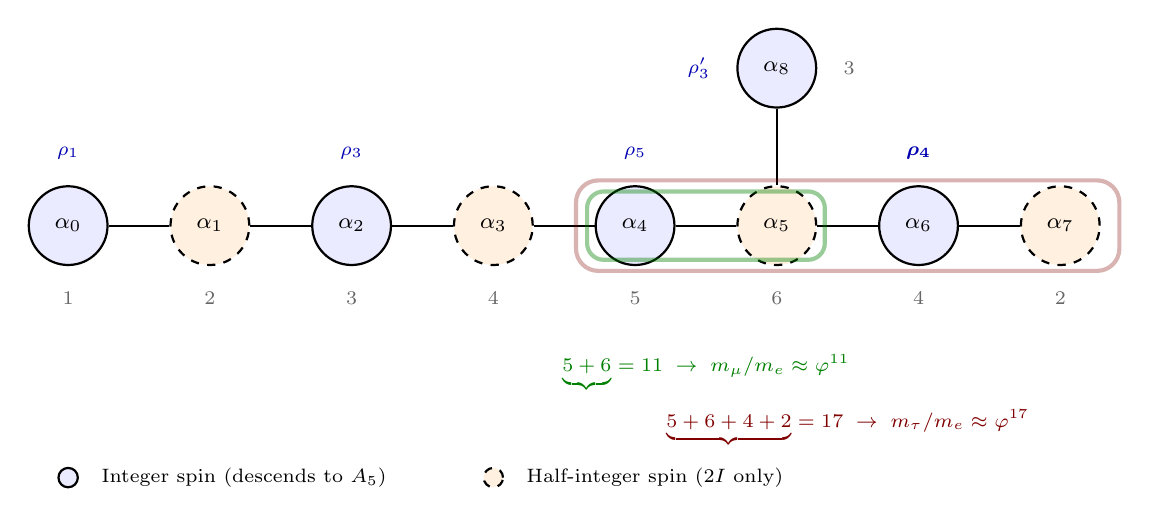
\begin{tikzpicture}[
  >=Stealth,
  int/.style={
    circle, draw, thick, minimum size=10mm,
    fill=blue!8, font=\footnotesize
  },
  half/.style={
    circle, draw, thick, minimum size=10mm,
    fill=orange!12, font=\footnotesize, dashed
  },
  dimlab/.style={font=\scriptsize, color=black!60},
  desclab/.style={font=\scriptsize\itshape, color=blue!70!black},
  edge/.style={thick},
]

%%% Main chain nodes — widened spacing (1.8cm)
\node[int]  (a0) at (0,0)     {$\alpha_0$};
\node[half] (a1) at (1.8,0)   {$\alpha_1$};
\node[int]  (a2) at (3.6,0)   {$\alpha_2$};
\node[half] (a3) at (5.4,0)   {$\alpha_3$};
\node[int]  (a4) at (7.2,0)   {$\alpha_4$};
\node[half] (a5) at (9.0,0)   {$\alpha_5$};
\node[int]  (a6) at (10.8,0)  {$\alpha_6$};
\node[half] (a7) at (12.6,0)  {$\alpha_7$};

%%% Branch node — above α5
\node[int]  (a8) at (9.0,2.0) {$\alpha_8$};

%%% Edges
\draw[edge] (a0) -- (a1);
\draw[edge] (a1) -- (a2);
\draw[edge] (a2) -- (a3);
\draw[edge] (a3) -- (a4);
\draw[edge] (a4) -- (a5);
\draw[edge] (a5) -- (a6);
\draw[edge] (a6) -- (a7);
\draw[edge] (a5) -- (a8);

%%% A5 descent labels (above integer-spin nodes, well separated)
\node[desclab, above=6pt of a0] {$\rho_1$};
\node[desclab, above=6pt of a2] {$\rho_3$};
\node[desclab, above=6pt of a4] {$\rho_5$};
\node[desclab, above=6pt of a6] {$\boldsymbol{\rho_4}$};
\node[desclab, left=6pt of a8]  {$\rho_3'$};

%%% Dimension labels (below each node, well below the circles)
\node[dimlab, below=6pt of a0] {$1$};
\node[dimlab, below=6pt of a1] {$2$};
\node[dimlab, below=6pt of a2] {$3$};
\node[dimlab, below=6pt of a3] {$4$};
\node[dimlab, below=6pt of a4] {$5$};
\node[dimlab, below=6pt of a5] {$6$};
\node[dimlab, below=6pt of a6] {$4$};
\node[dimlab, below=6pt of a7] {$2$};
\node[dimlab, right=6pt of a8] {$3$};

%%% Path annotations — below the dimension labels, no overlap
%%% Path to 11: α4 → α5  (5+6 = 11)
\draw[line width=1.5pt, color=green!50!black, opacity=0.4,
      rounded corners=6pt]
  ([xshift=-7pt, yshift=-2pt]a4.south west)
  rectangle
  ([xshift=7pt, yshift=2pt]a5.north east);
\node[font=\scriptsize, color=green!50!black, anchor=north]
  at ($(a4.south)!0.5!(a5.south) + (0,-1.0)$)
  {$\underbrace{5+6}_{} = 11 \;\to\; m_\mu/m_e \approx \varphi^{11}$};

%%% Path to 17: α4 → α5 → α6 → α7  (5+6+4+2 = 17)
\draw[line width=1.5pt, color=red!50!black, opacity=0.3,
      rounded corners=8pt]
  ([xshift=-11pt, yshift=-6pt]a4.south west)
  rectangle
  ([xshift=11pt, yshift=6pt]a7.north east);
\node[font=\scriptsize, color=red!50!black, anchor=north]
  at ($(a4.south)!0.5!(a7.south) + (0,-1.7)$)
  {$\underbrace{5+6+4+2}_{} = 17 \;\to\; m_\tau/m_e \approx \varphi^{17}$};

%%% Legend — bottom left, clear of annotations
\draw[thick, fill=blue!8]   (0,-3.2) circle (3.5pt);
\node[font=\scriptsize, anchor=west] at (0.3,-3.2)
  {Integer spin (descends to $A_5$)};
\draw[thick, dashed, fill=orange!12] (5.4,-3.2) circle (3.5pt);
\node[font=\scriptsize, anchor=west] at (5.7,-3.2)
  {Half-integer spin ($2I$ only)};

\end{tikzpicture}
\caption{McKay graph of the binary icosahedral group $2I$,
  corresponding to the affine Dynkin diagram $\hat{E}_8$.
  Solid circles (blue) denote integer-spin representations
  descending to $A_5$; dashed circles (orange) denote half-integer-spin
  representations unique to $2I$.
  Numbers below each node indicate the representation dimension.
  The branch point $\alpha_5$ (dim\,$6$) does not descend to $A_5$.
  The node $\alpha_6$ corresponds to $\rho_4$---the unique non-$\mathrm{SO}(3)$
  irreducible representation central to the selection rule~(P1).
  Shaded bands indicate the path sums yielding the $E_8$ Coxeter
  exponents $11$ and $17$, which match the charged lepton mass
  ratios $m_\mu/m_e \approx \varphi^{11}$ and
  $m_\tau/m_e \approx \varphi^{17}$}\label{fig:mckay}
\end{figure}

The numbers in parentheses are the dimensions of the $2I$-irreducible
representations, which correspond to the marks (Dynkin coefficients) of $E_8$
(Kostant).

\medskip
\noindent\textbf{Numerical consistency.}

\begin{table}[ht]
\caption{Numerical consistency between $E_8$ and the icosahedron. The Coxeter
number $h(E_8) = 30 = E$ is a necessary consequence of the McKay
correspondence.}\label{tab:E8-numerics}
\centering
\begin{tabular}{@{}ll@{}}
\toprule
Quantity & Value \\
\midrule
Mark sum $\sum m_i$           & $30 = E = h(E_8)$ (Coxeter number) \\
Mark sum of squares $\sum m_i^2$ & $120 = |2I|$ \\
$\dim(E_8)$                   & $248 = 8h + 8$ \\
Number of roots               & $240 = 4 \times |A_5|$ \\
\bottomrule
\end{tabular}
\end{table}

\noindent\textbf{$A_5$-node non-adjacency.}
On the McKay graph (Fig.~\ref{fig:mckay}), the integer-spin nodes
($\alpha_0, \alpha_2, \alpha_4, \alpha_6, \alpha_8$) descending to $A_5$ are
never adjacent---half-integer-spin nodes
($\alpha_1, \alpha_3, \alpha_5, \alpha_7$) always act as bridges.

\begin{table}[ht]
\caption{McKay graph structure for $\hat{E}_8$. $\alpha_6$ (corresponding to
$\rho_4$) is topologically special, one step from the branch point $\alpha_5$.
$\alpha_5$ (dimension $6 = \dim(\Lambda^2\rho_4)$) is unique to $2I$ and does
not descend to $A_5$.}\label{tab:mckay-graph}
\centering
\small
\begin{tabular*}{\textwidth}{@{\extracolsep{\fill}}lccll@{}}
\toprule
McKay node & Dim.\ & Spin & $A_5$ descent & Adjacent nodes \\
\midrule
$\alpha_0$ & 1 & Integer      & $\rho_1$  & $\alpha_1$ (half-int.) \\
$\alpha_1$ & 2 & Half-integer & \ding{55} & $\alpha_0,\,\alpha_2$ \\
$\alpha_2$ & 3 & Integer      & $\rho_3$  & $\alpha_1,\,\alpha_3$ \\
$\alpha_3$ & 4 & Half-integer & \ding{55} & $\alpha_2,\,\alpha_4$ \\
$\alpha_4$ & 5 & Integer      & $\rho_5$  & $\alpha_3,\,\alpha_5$ \\
$\alpha_5$ & 6 & Half-integer & \ding{55}
  & $\alpha_4,\,\alpha_6,\,\alpha_8$ \\
$\alpha_6$ & 4 & Integer      & $\rho_4$  & $\alpha_5,\,\alpha_7$ \\
$\alpha_7$ & 2 & Half-integer & \ding{55} & $\alpha_6$ \\
$\alpha_8$ & 3 & Integer      & $\rho_3'$ & $\alpha_5$ \\
\bottomrule
\end{tabular*}
\end{table}

The $\rho_4$ selection rule in Sect.~\ref{sec:P1}---``physical indices require
intersection with $\rho_4$''---can be interpreted as a
representation-theoretic reflection of the topological fact that the
$\alpha_6$ node occupies a privileged position on the McKay graph
(Fig.~\ref{fig:mckay}).


\subsection{\texorpdfstring{$E_8$}{E8} Coxeter exponents and charged lepton
masses}\label{app:coxeter-lepton}

The Coxeter exponents of $E_8$ are
$\mathrm{Exp}(E_8) = \{1, 7, 11, 13, 17, 19, 23, 29\}$. Only $\{11, 17\}$
belong to the allowed set $S_{\mathrm{allowed}}$, and the charged lepton mass
ratios $m_\mu/m_e \approx \varphi^{11}$, $m_\tau/m_e \approx \varphi^{17}$
(Appendix~\ref{app:observation}, \#12, \#13).

\begin{table}[ht]
\caption{Dual membership filter. Only $\{11, 17\}$ are simultaneously $E_8$
Coxeter exponents and independently derivable icosahedral combinations with
established physical correspondences.}\label{tab:dual-filter}
\centering
\small
\begin{tabular*}{\textwidth}{@{\extracolsep{\fill}}clll@{}}
\toprule
$E_8$ exponent & Icosahedral derivation & Physical quantity & Dual? \\
\midrule
1  & $\rho_1$ (trivial repr.)  & ---
   & \ding{55} \\
7  & $(E{+}V)/n - 7 = 7$      & ---
   & \ding{55} (no indep.\ $A_5$ deriv.) \\
11 & $\beta_0 = E/n + \chi/2 = 10 + 1$
   & $m_\mu/m_e \approx \varphi^{11}$
   & \ding{51} \\
13 & $V + 1$                   & ---
   & \ding{55} (no indep.\ phys.\ match) \\
17 & $F - n = 20 - 3$
   & $m_\tau/m_e \approx \varphi^{17}$
   & \ding{51} \\
19 & $F - 1$                   & ---
   & \ding{55} (no indep.\ phys.\ match) \\
23 & $F + n$                   & ---
   & \ding{55} (no indep.\ phys.\ match) \\
29 & $E - 1$                   & ---
   & \ding{55} (no indep.\ phys.\ match) \\
\bottomrule
\end{tabular*}
\end{table}

\noindent\textbf{Path structure on the McKay graph.}
The path sum starting from $\alpha_4$ ($\sigma_5 \to \rho_5$, dimension~5)
produces $\{11, 17\}$ (shaded bands in Fig.~\ref{fig:mckay}):
\begin{itemize}[nosep]
  \item $11 = m(\alpha_4) + m(\alpha_5) = 5 + 6$: shortest path to the branch
    point $\alpha_5$.
  \item $17 = m(\alpha_4) + m(\alpha_5) + m(\alpha_6) + m(\alpha_7)
    = 5 + 6 + 4 + 2$: entire path to the arm tip $\alpha_7$.
\end{itemize}
Both paths pass through the branch point $\alpha_5$ (a representation of
dimension $6$ unique to $2I$ that does not descend to $A_5$). The charged
lepton mass exponents $\{11, 17\}$ are thus simultaneously characterized in
three independent contexts: (i) the Coxeter exponents, (ii) physical
combinations of the icosahedron, and (iii) path sums on the McKay graph. We
leave the elucidation of the dynamical mechanism to G2.


\subsection{Path from \texorpdfstring{$E_8$}{E8} to the Standard Model}%
\label{app:E8-SM}

\noindent\textbf{Physical significance.}
Proposition~\ref{prop:2I-unique} implies that under postulates (H1)--(H3),
there is a uniquely determined $\mathrm{SU}(2)$ subgroup with a McKay
correspondence to $E_8$. $E_8$ has a special status in particle physics
($E_8 \times E_8$ in heterotic strings, singularities in F-theory), and this
paper provides a new context in which $E_8$ emerges naturally from holonomy
constraints on external spaces.

\medskip
\noindent\textbf{Candidate route.}
The typical GUT branching chain is
\[
  E_8 \supset E_6 \supset \mathrm{SO}(10) \supset \mathrm{SU}(5)
  \supset \mathrm{SU}(3) \times \mathrm{SU}(2) \times \mathrm{U}(1)\,.
\]
The connection path of this paper is
\[
  A_5
  \;\xrightarrow{\text{Klein}}\;
  2I
  \;\xrightarrow{\text{McKay}}\;
  E_8
  \;\xrightarrow{\text{GUT}}\;
  \text{SM}\,.
\]
The first two steps (Klein $\to$ McKay) are mathematically rigorous and have
been formally verified. The third step (GUT branching) is a physical hypothesis
beyond the scope of this paper.

\medskip
\noindent\textbf{Consistency with superstring theory.}
While the above GUT branching chain is a field-theoretic pathway, superstring
theory provides independent mechanisms for realizing $E_8$: gauge enhancement
at ADE singularities, anomaly cancellation in heterotic strings, and singular
fiber degeneracy in F-theory. Our $2I$ (the input of the McKay correspondence)
has an entry point consistent with all of these mechanisms. Details are given
in Appendix~\ref{app:string}. This consistency is not an extension of our
claims, but a confirmation that the $A_5 \to 2I \to E_8$ chain is consistent
with the known framework of string theory.

\medskip
\noindent\textbf{The essential difficulty.}
The $A_5$ holonomy in this paper constrains the exterior space (spatial frame
bundle) and does not directly determine the interior gauge symmetry
$\mathrm{SU}(3) \times \mathrm{SU}(2) \times \mathrm{U}(1)$. Three elements
are necessary for the connection, and all remain unsolved (G1$'$).

\begin{table}[ht]
\caption{Three unresolved elements for the external--internal connection
(G1$'$).}\label{tab:G1-elements}
\centering
\begin{tabular}{@{}p{3cm}p{5.5cm}p{5.5cm}@{}}
\toprule
Unresolved element & Content & Candidate approaches \\
\midrule
External--internal connection
  & $A_5$ holonomy $\to$ dynamical derivation of gauge group
  & Kaluza--Klein, spectral geometry \\
Action functional
  & Constructing actions consistent with finite group holonomies
  & Extension of Dijkgraaf--Witten theory~\cite{DijkgraafWitten90} \\
Continuum limit
  & Discrete holonomy $\to$ emergence of continuous fields
  & Gauge--Higgs unification model \\
\bottomrule
\end{tabular}
\end{table}

The challenge is not to ``derive the gauge group of the SM,'' but to
understand why the algebraic rigidity of $A_5$ produces SM-like phenomena at
low energies.


\subsection{Systematic comparison with the Swampland program}%
\label{app:swampland}

The structural consistency with the Swampland conditions, briefly described in
Sect.~\ref{sec:H3} of the main text, is systematically listed below.

\begin{table}[ht]
\caption{Systematic comparison of $A_5$ holonomy with Swampland
conjectures.}\label{tab:swampland}
\centering
\scriptsize
\setlength{\tabcolsep}{3pt}
\begin{tabular*}{\textwidth}{@{\extracolsep{\fill}}lp{2.0cm}p{2.2cm}p{2.5cm}p{2.5cm}@{}}
\toprule
Swampland conjecture & Content & Relation to $A_5$
  & Satisfaction mechanism & What is not claimed \\
\midrule
No-Global-Symmetries \cite{BanksDixon,HarlowOoguri}
  & No global symmetry in QG
  & (H3) $\Hab = 1$ prohibits automatic charges
  & Direct consequence of $\Hab = 1$; $A_4$ ($\mathbb{Z}_3$) and $S_4$
    ($\mathbb{Z}_2$) eliminated
  & Proof for continuous gauge theories \\
Cobordism \cite{McNamaraVafa}
  & Cobordism group is trivial
  & No nontrivial $H \to \mathrm{U}(1)$ (equivalent to $\Hab = 1$)
  & Direct consequence of $\Hab = 1$
  & Complete cobordism computation; strict equivalence \\
Weak Gravity
  & Gravity is the weakest force
  & $\alpha/\alpha_G = \varphi^{204} \sim 10^{44}$
  & Hierarchy describable in $A_5$ algebra; quantitative agreement not
    guaranteed
  & Rigorous WGC bound derivation \\
Distance
  & Infinite tower at large moduli distances
  & Discrete holonomies have no continuous moduli
  & Premise of conjecture is absent
  & Moduli analysis in continuum limit \\
Finiteness
  & EFT landscape is finite
  & Klein's classification limits candidates to five; (H1)--(H3) unify to one
  & Algebraic finiteness
  & Counting string vacua \\
\bottomrule
\end{tabular*}
\end{table}

\noindent\textbf{Classification of satisfaction patterns.}
The satisfaction of the five Swampland conditions by $A_5$ holonomy can be
classified into three distinct mechanisms.

\begin{enumerate}[nosep,label=(\roman*)]
  \item \textbf{Automatic algebraic sufficiency (No-Global-Symmetries,
    Cobordism).}
    The single algebraic condition $\Hab = 1$---postulate (H3) itself---automatically
    satisfies the discrete versions of both conjectures simultaneously.

  \item \textbf{Obvious absence of premise (Distance).}
    Since discrete holonomy models have no continuous moduli, the assumptions
    of the Distance Conjecture do not apply.

  \item \textbf{Algebraic description only (Weak Gravity).}
    The hierarchy $\alpha/\alpha_G \sim \varphi^{204}$ can be described in
    $A_5$ algebra, but strict agreement with the quantitative bound of WGC has
    not been verified.
\end{enumerate}

\noindent\textbf{Global symmetry prohibition in discrete geometry.}
In continuous gauge theories, the No-Global-Symmetries conclusion is reached
via dynamical arguments (such as the black hole no-hair theorem). In discrete
holonomies, it is directly enforced by the algebraic structure $\Hab = 1$.
When $\Hab \neq 1$, discrete topological charges for closed-curve holonomies
are automatically defined independent of dynamics ($\mathbb{Z}_3$ charges in
$A_4$, $\mathbb{Z}_2$ signs in $S_4$). Postulate (H3) eliminates this
algebraically.


\subsection{Comparison with Lisi's \texorpdfstring{$E_8$}{E8} unified theory}%
\label{app:lisi}

Lisi (2007)~\cite{Lisi07} proposed unifying all Standard Model particles
into a single Lie algebra by starting directly from the root system of $E_8$.
This approach is fundamentally different from ours in starting point, the
status of $E_8$, methodology, and principal difficulties.

\begin{table}[ht]
\caption{Comparison with Lisi's $E_8$ theory.}\label{tab:lisi}
\centering
\begin{tabular}{@{}lll@{}}
\toprule
  & This paper & Lisi (2007) \\
\midrule
$E_8$ status
  & $A_5 \to 2I \to$ McKay consequence
  & Direct assumption \\
Starting point
  & 3D (H1)(H2)(H3) + frame bundle
  & $E_8$ root system + 248-dim.\ rep. \\
SM connection
  & Unresolved (G1$'$)
  & Asserted via 248 embedding \\
Formal verification
  & Lean~4 ($\mathtt{sorry} = 0$)
  & None \\
Main difficulty
  & External--internal gap
  & Non-embeddability (Distler--Garibaldi) \\
Scope
  & Conditional theorem
  & Theory of Everything \\
\bottomrule
\end{tabular}
\end{table}

\noindent\textbf{Relationship with the Distler--Garibaldi criticism.}
The central argument of Distler--Garibaldi~\cite{DistlerGaribaldi09} against Lisi's
proposal was that it is representationally impossible to embed the full
particle content of the Standard Model consistently in the root system of
$E_8$. Specifically, the generation structure of fermions and the branching of
$E_8$ representations are incompatible.

Our approach is structurally different from the object of this criticism. We do
not directly embed particles in the $E_8$ root system (we work only with
mathematical facts via the McKay correspondence), and we classify the SM
connection as unsolved (G1$'$). All representation-theoretic calculations are
formally verified in Lean~4, and our claims are explicitly restricted to
conditional theorems.


\subsection{Physical and mathematical contexts in which
\texorpdfstring{$A_5$}{A5} appears independently}\label{app:independent}

$A_5$ (the icosahedral group) has a privileged status in multiple physical and
mathematical contexts, independent of the three postulates of this paper. The
following is an overview, emphasizing that each connection was discovered
independently of our framework.


\subsubsection{Fibonacci anyons and topological quantum computing}%
\label{app:fibonacci}

The Fibonacci anyon fusion rule in $2{+}1$-dimensional topological order,
$\tau \times \tau = 1 + \tau$, is closely related to the representation theory
of $A_5$. The image of the braid group in $\mathrm{SU}(2)$ Chern--Simons
theory (level $k = 3$) is homomorphic to $A_5$~\cite{FibAnyon08}, and
Fibonacci anyon braiding provides a minimal model for universal quantum
computation.

The physical significance is that the non-solvability of $A_5$ is directly
linked to the universality of quantum computation: solvable groups alone limit
the simulation capabilities of quantum circuits---this can be seen as the
quantum analogue of solvable opacity (Theorem~\ref{thm:opacity} in
Sect.~\ref{sec:solvable-opacity}) and Barrington's theorem
(Appendix~\ref{app:unified-barrier}).


\subsubsection{Barrington's theorem and Krohn--Rhodes theory}%
\label{app:barrington-ref}

As detailed in Appendix~\ref{app:unified-barrier}, $A_5$ is the critical
instruction set for width-5 branching programs in computational complexity
(Barrington~\cite{Barrington89}) and the smallest ``non-solvable prime'' of
a finite semigroup (Krohn--Rhodes~\cite{KrohnRhodes65}). These results were
discovered purely within the theory of computation and algebra, independent of
any physical motivation.


\subsubsection{Universality of the ADE classification}\label{app:ADE}

$2I \to E_8$ corresponds to the most exceptional type in the ADE
classification and appears universally in the following contexts.

\begin{table}[ht]
\caption{Universality of the ADE classification and the icosahedral
connection.}\label{tab:ADE}
\centering
\small
\begin{tabular}{@{}lll@{}}
\toprule
ADE context & Appearance of $E_8$ & Icosahedral connection \\
\midrule
Simple Lie algebras
  & $E_8$ is the most exceptional
  & $2I$ generates $\hat{E}_8$ via McKay \\
Surface singularity resolution
  & $E_8$-type singularity
  & Orbifold $\mathbb{C}^2/2I$ \\
Heterotic strings
  & $E_8 \times E_8$ gauge group
  & 10D anomaly cancellation \\
F-theory
  & $E_8$ singular fiber
  & Compactification geometry \\
Finite subgroup classification
  & ADE-compatible maximal example
  & $2I$ is the largest exceptional subgroup \\
\bottomrule
\end{tabular}
\end{table}

The universality of the ADE classification shows that the privileged position
of $E_8$ has a mathematical necessity independent of the three postulates of
this paper.


\subsubsection{Monstrous Moonshine}\label{app:moonshine}

$A_5$ is a subgroup of the Monster group $\mathbb{M}$, and McKay's $E_8$
observation---that $E_8$ is involved in the factorization of 196883 in the
first nontrivial representation of the Monster character table,
$196884 = 1 + 196883$---is positioned as part of the $2I \to E_8$ connection
and the Moonshine phenomenon. However, a concrete dynamical connection between
the framework of this paper and Moonshine has not been established.


\subsubsection{Quasicrystals and non-periodic structures}%
\label{app:quasicrystals}

Icosahedral symmetry in three-dimensional space appears directly in materials
science as the symmetry of the Penrose tiling (two-dimensional) and
quasicrystals (three-dimensional, Shechtman 1984). The five-fold symmetry of
quasicrystal diffraction patterns is a geometric realization of $A_5$, and the
golden ratio $\varphi$ appears in the lattice parameters.


\subsubsection{Viral capsid structure}\label{app:virus}

According to the Caspar--Klug theory (1962), most viral capsids (outer shells)
exhibit icosahedral symmetry $A_5$. The T-number (triangulation number)
classification is based on the triangulation of icosahedral faces, and the
smallest viral capsids ($T = 1$, 60 subunits) directly reflect the $A_5$
orbit structure.


\subsubsection{Implications of independent occurrence}%
\label{app:implications}

The above contexts were discovered independently of each other and are
independent of the three postulates of this paper. The privileged status of
$A_5/2I/E_8$ in such a wide variety of contexts suggests that the starting
point of this paper (uniqueness via (H1)--(H3)) is not an arbitrary choice but
may have reached a mathematically deep structure. However, ``appearing in many
contexts'' does not prove ``physically correct,'' and the epistemological
reservation in Sect.~\ref{sec:conclusion} applies.


%% ============================================================
%% APPENDIX D: Information Barriers, Entropy, and Irreversibility
%% ============================================================
\section{Information Barriers, Entropy, and Irreversibility}\label{app:entropy}

This appendix details the physical implications of the information barrier
briefly mentioned in Sect.~\ref{sec:solvable-opacity} (solvable opacity).

\medskip
\noindent\textbf{Epistemological note.}
The cumulative barrier, minimality, and fiber decomposition in
Sect.~\ref{app:barrier-quant} are formally verified algebraic facts (Layer~M). The
physical interpretations in
Sects.~\ref{app:boltzmann}--\ref{app:bekenstein} belong to Layer~P/E and are
speculative. The logical validity of the conditional theorems
(Sect.~\ref{sec:main-theorem}) and the prohibition structure
(Sect.~\ref{sec:prohibition}) in the main text is independent of the success or
failure of the speculative interpretations in this appendix.


\subsection{Quantitative structure of the \texorpdfstring{$60^N$}{60\^{}N}
information barrier}\label{app:barrier-quant}

From Corollary~\ref{cor:degeneracy} and Corollary~\ref{cor:minimal-barrier},
the barriers to solvable observation for $A_5$ have the following hierarchy:

\begin{enumerate}[nosep,label=(I-\alph*)]
  \item \textbf{Existence.}
    Any solvable probe $\pi \colon A_5 \to Q$ satisfies $\ker(\pi) = A_5$,
    and 60 microscopic states are mapped to a single observable.
    \emph{[Verified.]}
  \item \textbf{Accumulation.}
    The cumulative ambiguity over $N$ steps grows exponentially to
    $60^N \geq 2^{5N}$ ($\geq \log_2 60 \approx 5.91$ bits of information
    loss per step). \emph{[Verified.]}
  \item \textbf{Minimality.}
    All finite groups of order less than 60 are solvable and have zero barrier.
    $A_5$ defines the minimal basis for irreversibility. \emph{[Verified.]}
\end{enumerate}

(I-a)--(I-c) are pure group-theoretic facts (supported by the classification
of finite simple groups~\cite{GLS94} and the Feit--Thompson odd-order
theorem~\cite{FeitThompson63}) and do not depend on physical hypotheses.

\medskip
\noindent\textbf{Fiber decomposition.}
By the orbit--stabilizer decomposition in Sect.~\ref{sec:orbit-stab}, $60^N$
admits three fiber decompositions.

\begin{table}[ht]
\caption{Three fiber decompositions of the $60^N$ information barrier. The
total per step ($\log_2 60 \approx 5.91$ bits) is invariant across sectors;
only the orbit/stabilizer partition differs.}\label{tab:fiber}
\centering
\begin{tabular*}{\textwidth}{@{\extracolsep{\fill}}llcccc@{}}
\toprule
Sector & Geom.\ object & Stabilizer & Orbit bits & Stab.\ bits & Total \\
\midrule
Face (electromagnetic)
  & $F = 20$ & $\mathbb{Z}_3$ & $\approx 4.32$ & $\approx 1.58$ & 5.91 \\
Edge (strong force)
  & $E = 30$ & $\mathbb{Z}_2$ & $\approx 4.91$ & $1.00$         & 5.91 \\
Vertex (gravity)
  & $V = 12$ & $\mathbb{Z}_5$ & $\approx 3.58$ & $\approx 2.32$ & 5.91 \\
\bottomrule
\end{tabular*}
\end{table}

There is an anti-correlation between stabilizer-group size (local confinement
information) and coupling strength---consistent with the vertex sector
(gravitational candidate), which has the largest stabilizer $\mathbb{Z}_5$,
being the weakest force. However, the sector correspondence depends on the
working hypothesis (C1), and a first-principles derivation has not been
achieved (G3).


\subsection{Group-theoretic reinterpretation of Boltzmann entropy}%
\label{app:boltzmann}

In Boltzmann's $S = k_B \ln W$, statistical mechanics explains why $W$ is
large by comparing phase-space volumes, but the origin of
coarse-graining---why microscopic states become indistinguishable---is usually
accepted as a premise. The solvable opacity of $A_5$ gives an algebraic
specification to this origin. Since $\ker(\pi) = A_5$, in $N$ steps:
\begin{equation}\label{eq:boltzmann}
  W_N = 60^N\,,\qquad
  S_N = N\,k_B \ln 60 \approx 4.094\,N\,k_B\,.
\end{equation}
Since $A_5$ is the smallest non-solvable group (I-c), $\ln 60$ defines the
smallest nontrivial lower bound on information loss.

\medskip
\noindent\textbf{Connection with statistical mechanics.}
The $A_5$ framework does not deny statistical mechanics but provides a
foundation for it.
$W_{\mathrm{total}} \geq W_{\mathrm{dyn}} \times 60^N$, where $60^N$ is an
algebraic factor independent of mechanical details, and $W_{\mathrm{dyn}}$ is
the conventional phase-space partitioning factor. Ordinary statistical
mechanics deals only with $W_{\mathrm{dyn}}$, and $60^N$ is hidden in the
background as the basis for coarse-graining. While Penrose's Past Hypothesis
asks ``Why did we start from low entropy?'', the $A_5$ framework addresses a
logically prior question: ``Why is the concept of entropy definable at all?''


\subsection{Fourth answer to the Loschmidt paradox}\label{app:loschmidt}

The $A_5$ framework provides an algebraic answer that is qualitatively
different from the three previous answers (Past Hypothesis, typicality, and
branching). For microscopic dynamics $g \in A_5$, $g^{-1}$ exists and
mechanical reversibility is maintained. However, under any solvable probe
$\ker(\pi) = A_5$, so $g$ and $g^{-1}$ become indistinguishable, and the
information required to select the ``correct inversion operation'' vanishes due
to the cumulative ambiguity of $60^N$ in $N$ steps.

If $|H| < 60$, $H$ is solvable, a faithful solvable probe exists, and
perfect observational reversibility is maintained. \emph{[Verified.]}

\begin{table}[ht]
\caption{Four answers to the Loschmidt paradox. The $A_5$ answer addresses the
logically prior question of why coarse-graining produces
irreversibility.}\label{tab:loschmidt}
\centering
\begin{tabular}{@{}lll@{}}
\toprule
Answer & Question addressed & Nature \\
\midrule
Past Hypothesis   & Why low initial $S$?          & Factual \\
Typicality        & Why is $S$-growth typical?    & Measure-theoretic \\
Branching         & Why does the future diverge?  & Coarse-graining dependent \\
$A_5$ answer      & Why does coarse-graining lose information?
                  & Algebraic \\
\bottomrule
\end{tabular}
\end{table}


\subsection{Formal connection with the cosmological constant and the
Bekenstein upper bound}\label{app:bekenstein}

For $\Lambda \ell_{\mathrm{Pl}}^2 \sim \varphi^{-600}$
(Appendix~\ref{app:observation}, \#39), the exponent 600 has a consistent
factorization from information barrier parameters:
\begin{equation}\label{eq:600}
  600 = |A_5| \times 10 = 2 \times 291 + (E - V)\,.
\end{equation}

Internal consistency of the $\Lambda$--$H_0$ relation:
$\varphi^{-600} = (\varphi^{-291})^2 \times \varphi^{-18}
= \varphi^{-582 - 18} = \varphi^{-600}$. \ding{51}

\medskip
Postulates (H1) (finite holonomy) and (H3*) (solvable opacity) independently
guarantee two essential properties of entropy:

\begin{table}[ht]
\caption{Dual guarantee of entropy properties from (H1) and
(H3*).}\label{tab:entropy-dual}
\centering
\begin{tabular}{@{}lll@{}}
\toprule
Physical principle & Group-theoretic correspondence & Entropy consequence \\
\midrule
(H1) Finite holonomy
  & $N < \infty$
  & $S \leq N\,k_B \ln 60 < \infty$ (finiteness) \\
(H3*) Solvable opacity
  & $|\ker(\pi)| = 60 > 1$
  & $dS/dN = k_B \ln 60 > 0$ (monotone increase) \\
\bottomrule
\end{tabular}
\end{table}


\subsection{Testability and experimental perspectives}\label{app:testability}

The crucial difference between the $A_5$ answer and existing answers is the
prediction of an irreversibility threshold:
$|H| < 60 \;\Rightarrow\;$ information barrier $= 0 \;\Rightarrow\;$ no
observational irreversibility.

\begin{enumerate}[nosep,label=(\roman*)]
  \item \textbf{Quantum simulator.}
    Comparing the qualitative difference in entropy production rates between
    $A_5$ anyon systems and solvable anyon systems (e.g., $\mathbb{Z}_5$). The
    Fibonacci anyon model (Appendix~\ref{app:fibonacci}) is the smallest
    experimental system. [G6]
  \item \textbf{Discrete gauge theory.}
    Comparison of phase transition structures between $\mathbb{Z}_5$ gauge
    theory (solvable) and $A_5$ gauge theory (non-solvable) on the lattice.
    [G6]
  \item \textbf{Topological quantum computing.}
    Barrington's theorem~\cite{Barrington89} mathematically guarantees a
    qualitative difference in computational power between solvable gauge groups
    and those including $A_5$. Whether this difference is physically realized
    as a difference in entropy production rates is not yet clear. [G6]
\end{enumerate}


\subsection{Epistemological summary}\label{app:entropy-epistemology}

\begin{table}[ht]
\caption{Epistemological classification of Appendix~\ref{app:entropy}
claims.}\label{tab:entropy-claims}
\centering
\small
\begin{tabular}{@{}p{4.5cm}cp{5.5cm}@{}}
\toprule
Claim & Layer & Verification status \\
\midrule
Cumulative barrier $60^N \geq 2^{5N}$
  & M & Lean~4 formally verified \\
Minimality ($|G| < 60 \Rightarrow G$ solvable)
  & M & Lean~4 formally verified \\
Three fiber decompositions
  & M & Lean~4 formally verified \\
Boltzmann reinterpretation ($60^N =$ coarse-graining lower bound)
  & P & Speculative \\
Loschmidt's 4th answer (non-solvability $\to$ irreversibility)
  & P & Speculative \\
Cosmological constant connection ($600 = 2 \times 291 + 18$)
  & E & Numerical consistency only \\
Bekenstein upper bound consistency
  & P & Speculative \\
\bottomrule
\end{tabular}
\end{table}

The conditions for falsifying Layer~M---(a) the discovery of a non-solvable
group of order $< 60$, (b) the construction of a faithful solvable probe of
$A_5$---have been virtually ruled out by existing mathematical theorems. The
conditions for falsifying Layer~P/E---(c) the demonstration of a
fundamentally reversible macroscopic process, (d) significant deviation between
$\Lambda \ell_{\mathrm{Pl}}^2$ and $\varphi^{-600}$---are physically open
questions left to future experiments and observations.


%% ============================================================
%% APPENDIX E: Five Cosmic Constraints — A Unified View
%% ============================================================
\section{Five Cosmic Constraints --- A Unified View}\label{app:five-cc}

This appendix presents the formulation (Sect.~\ref{app:cc-formulation}) of the
Five Cosmic Constraints (CC1)--(CC5) outlined in Sect.~\ref{sec:conditional-structure}
of the main text, their logical hierarchy (Sect.~\ref{app:cc-hierarchy}),
interrelationships and independence (Sect.~\ref{app:cc-independence}), and a
unified perspective with epistemological summary (Sect.~\ref{app:cc-unified}).

\medskip
\noindent\textbf{Methodological note.}
The five constraints are structural patterns that emerge when the individual
results of Sects.~\ref{sec:main-theorem}--\ref{sec:limitations} are viewed
collectively. Each constraint has a different epistemological status (a mixture
of Layers~M/P/E), and this difference must not be obscured.


\subsection{Formulation of the five constraints}\label{app:cc-formulation}

The non-solvability of $A_5$ leads to five hierarchical ``cosmic
constraints.''

\medskip
\noindent\textbf{CC1: Information barriers and irreversibility.}
Under $A_5$ holonomy, solvable observations introduce a structural ambiguity
of $|\ker(\pi)| = 60$ at each step, creating a cumulative information barrier
of $60^N \geq 2^{5N}$ over $N$ steps. This barrier is an algebraic necessary
condition for irreversibility and vanishes in solvable universes with
$|H| < 60$.

\emph{Physical scope:} A possible group-theoretic basis for the second law of
thermodynamics; a fourth answer to the Loschmidt paradox
(Appendix~\ref{app:loschmidt}).

\emph{Refutation condition:} Demonstration of a macroscopic process that is
reversible in principle. (The algebraic facts (I-a)--(I-c) themselves cannot be
falsified.)

\medskip
\noindent\textbf{CC2: Symmetry segmentation and the origin of conservation
laws.}
The action of $A_5 \cong \mathrm{Rot}(\text{Icosahedron})$ on the
icosahedron uniquely defines three orbits ($F = 20$, $E = 30$, $V = 12$) and
stabilizer groups ($\mathbb{Z}_3$, $\mathbb{Z}_2$, $\mathbb{Z}_5$), providing
a discrete pre-structure for the three force sectors
(Sect.~\ref{sec:orbit-stab}). The absence of automatic charges due to $\Hab = 1$
can be read as a discrete version of the No-Global-Symmetries Conjecture
(Sect.~\ref{sec:H3}).

\emph{Refutation conditions:} (a) Discovery of microscopic universal discrete
conserved quantities $\to$ (H3) refutation. (b) Discovery of a fourth
fundamental force. (c) Empirical denial of the correspondence rule (C1).

\medskip
\noindent\textbf{CC3: Prohibition structure (algebraic exclusion principle).}
The representation theory of $A_5$ defines a threefold prohibition structure
for $\varphi$-power exponents: (P1) the $\rho_4$ tensor-product selection rule
(10/10 exact match, Sect.~\ref{sec:P1}), (P2) the multiplicity-free condition
(7/8 match, Sect.~\ref{sec:P2}), and (P3) the $E_8$ Coxeter-exponent filter
(Sect.~\ref{sec:P3}). The pre-specification of the forbidden exponents
$\{9, 15, 16, 25\}$ provides a falsifiable prediction.

\emph{Refutation condition:} Discovery of stable $\varphi^p$ relations
corresponding to forbidden exponents. Among the five constraints, CC3 has the
sharpest falsifiability.

\medskip
\noindent\textbf{CC4: Necessity of scale hierarchy.}
The icosahedral parameters $(F, E, V, n) = (20, 30, 12, 3)$ uniquely
determine the exponents of all physical scale hierarchies.
$H_G = V(F - n) = 204$ (gravitational--electromagnetic hierarchy) is an
inevitable consequence of $|A_5| = 60$, and the question ``why this
hierarchy?'' reduces to ``why $A_5$?'' All exponents belong to
$S_{\mathrm{allowed}}$, which is closed under integer arithmetic on the
icosahedral parameters.

\emph{Refutation conditions:} (a) Discovery of an algebraic structure that
realizes an equivalent hierarchy in $n \neq 3$. (b) Discovery of a new scale
hierarchy that cannot be described by $S_{\mathrm{allowed}}$.

\medskip
\noindent\textbf{CC5: Cosmological consistency.}
The microscopic and macroscopic $\varphi$-exponents are consistently connected
by integer relations in the icosahedral parameters. The cosmological relation
$\Lambda \sim H_0^2$ is automatically satisfied as an internal consistency
condition of the $A_5$ algebra: $600 = 2 \times 291 + (E - V)$,
$204 = V \times (F - n)$, $\beta_0 = E/n + \chi/2 = 11$.

\emph{Refutation condition:} Precision measurements of $\Lambda$ and $H_0$
establish systematic deviations from $\varphi^{-600}$ and $\varphi^{-291}$.


\subsection{Logical hierarchy}\label{app:cc-hierarchy}

From the non-solvability of $A_5$, three algebraic mechanisms diverge and
crystallize into the five constraints.

\begin{center}
\small
\begin{tabular}{@{}c@{}}
Non-solvability of $A_5$ \;($|A_5| = 60$, smallest non-solvable) \\[4pt]
$\swarrow$ \hspace{6em} $\downarrow$ \hspace{6em} $\searrow$ \\[2pt]
\begin{tabular}{@{}c@{\hspace{3em}}c@{\hspace{3em}}c@{}}
Total degeneracy & Orbit--stabilizer & Representation \\
$\ker(\pi) = A_5$ & $60 = F{\cdot}3 = E{\cdot}2 = V{\cdot}5$
  & $\rho_3 \to \varphi \to \mathrm{gap}$ \\
(Mechanism 1) & (Mechanism 2) & (Mechanism 3)
\end{tabular} \\[4pt]
$\downarrow$ \hspace{8em} $\downarrow$ \hspace{8em} $\downarrow$ \\[2pt]
\textbf{CC1:} Info.\ barrier \hspace{2em}
\textbf{CC2:} Segmentation \hspace{2em}
\textbf{CC3:} Prohibition \\[4pt]
$\searrow$ \hspace{3em} $\downarrow$ \hspace{3em} $\swarrow$ \\[2pt]
\textbf{CC4:} Scale hierarchy \\[4pt]
$\downarrow$ \\[2pt]
\textbf{CC5:} Cosmological consistency
\end{tabular}
\end{center}

CC1--CC3 arise from the non-solvability of $A_5$ through three independent
algebraic mechanisms. CC4 arises as a quantitative synthesis of CC1--CC3
(barrier ``depth'' + sector structure + prohibition filter), and CC5 is an
extension of CC4 to the macroscale.


\subsection{Interrelationships and logical independence}%
\label{app:cc-independence}

\noindent\textbf{Independence.}

\begin{table}[ht]
\caption{Logical relationships among the five constraints.}\label{tab:cc-rels}
\centering
\begin{tabular}{@{}lll@{}}
\toprule
Pair & Relation & Basis \\
\midrule
CC1 $\leftrightarrow$ CC2
  & Independent
  & CC1 depends only on non-solvability; CC2 only on orbit decomposition \\
CC1 $\leftrightarrow$ CC3
  & Independent
  & Group-theoretic kernel structure vs.\ representation-theoretic
    tensor products \\
CC2 $\leftrightarrow$ CC3
  & Independent
  & Geometric group action vs.\ internal structure of the representation
    ring \\
CC4 $\leftarrow$ CC1--CC3
  & Subordinate
  & Combines barrier + prefactor + prohibition structure \\
CC5 $\leftarrow$ CC4
  & Subordinate
  & Extension to cosmological scales \\
\bottomrule
\end{tabular}
\end{table}

\noindent\textbf{Refutation cascade structure.}

\begin{table}[ht]
\caption{Refutation cascade. Rejection of any CC1--CC3 does not affect the
others. Rejection of CC4/CC5 has no upstream effect. The five constraints can
be verified and refuted individually, not collectively.}\label{tab:cc-cascade}
\centering
\begin{tabular}{@{}lll@{}}
\toprule
Rejected & Downstream effect & Unaffected \\
\midrule
CC1 & CC4 loses ``depth'' control    & CC2, CC3 unaffected \\
CC2 & CC4 loses sector structure     & CC1, CC3 unaffected \\
CC3 & CC4 loses prohibition filter   & CC1, CC2 unaffected \\
CC4 & CC5 loses its premise          & CC1--CC3 unaffected \\
CC5 & None (terminal node)           & CC1--CC4 unaffected \\
\bottomrule
\end{tabular}
\end{table}


\subsection{Unified perspective and epistemological summary}%
\label{app:cc-unified}

The five constraints ultimately reduce to a single proposition:
\begin{quote}
\itshape
$A_5$ (the alternating group of order $60$) is the smallest non-solvable
element in the classification of finite simple groups.
\end{quote}

Although these consequences were formulated independently, they derive from a
single structure, $A_5$. This convergence reinforces the motivation for
research into G1$'$ (emergence problem) and G6 (physical realization).

\begin{table}[ht]
\caption{Unified summary of the five cosmic constraints. Although formulated
independently, all derive from the single algebraic structure of
$A_5$.}\label{tab:cc-summary}
\centering
\small
\begin{tabular*}{\textwidth}{@{\extracolsep{\fill}}lp{2.8cm}p{2.8cm}cp{1.2cm}@{}}
\toprule
Constraint & Consequence & Physical interpretation & Layer
  & Falsif. \\
\midrule
CC1 & Information barrier ($60^N$)
  & Possible algebraic basis for the arrow of time
  & M+P & Medium \\
CC2 & Three-sector force division
  & Discrete pre-structure of Noether's theorem
  & M+(C1) & High \\
CC3 & $\varphi$-power prohibition structure
  & Analogue of the Pauli exclusion principle
  & M & Highest \\
CC4 & Icosahedral arithmetic of scale hierarchies
  & Possible answer to the hierarchy problem
  & M+E & Medium \\
CC5 & Micro--macro cosmological alignment
  & Automatic satisfaction of the $\Lambda$--$H_0$ relation
  & M+E & Medium \\
\bottomrule
\end{tabular*}
\end{table}

\noindent\textbf{Explicit non-claim.}
The five constraints do not claim any dynamical mechanism that ``determines''
the structure of the universe. They are presented as conditional consequences,
and each constraint can be evaluated and falsified independently (see
Sect.~\ref{app:cc-independence}).


%% ============================================================
%% APPENDIX F: String Theory Compatibility via E8
%% ============================================================
\section{String Theory Compatibility via \texorpdfstring{$E_8$}{E8}}%
\label{app:string}

\subsection{Purpose and scope}\label{app:string-purpose}

This appendix builds on the mathematical chain established in Sect.~\ref{sec:P3}
and Appendix~\ref{app:mckay}:
\[
  A_5
  \;\xrightarrow{\text{Klein}}\;
  2I
  \;\xrightarrow{\text{McKay}}\;
  \hat{E}_8\,,
\]
and checks its structural consistency with the standard constructions of
superstring theory. This is not a new physical claim but a compatibility check
with known string-theoretic mechanisms.

Note that the McKay correspondence directly gives the affine type $\hat{E}_8$,
whereas in string theory ``gauge algebra $E_8$'' usually refers to the finite
Lie algebra $E_8$ (the finite part with the affine node removed). This
appendix carefully distinguishes the two.

\medskip
\noindent\textbf{Explicit non-claims.}
This appendix only presents the structural fact that the mathematical chain
$A_5 \to 2I \to E_8$ shares an isomorphic entry point with independent
mechanisms on the string theory side. It does not claim the correctness of
superstring theory, a string-theoretic derivation of the $A_5$ holonomy, or a
derivation of the SM gauge group.

\medskip
\noindent\textbf{Layer classification.}
This appendix belongs to the boundary between Layer~M and Layer~P. The
mathematics of ``obtaining $E_8$ from $2I$''---the McKay correspondence, the
algebraic geometry of Du Val/ADE singularities, and the Dechant
construction---belongs to Layer~M. The interpretation that ``it is realized as
an effective gauge symmetry of string theory'' belongs to Layer~P and does not
solve the emergence problem G1$'$ in the main text.


\subsection{Three compatibility paths}\label{app:three-paths}

Our $2I$ (the binary icosahedral group) has an entry point consistent with the
following three standard mechanisms in superstring theory.


\subsubsection{Path~I: ADE singularity and gauge enhancement}%
\label{app:path-I}

In string theory, if the internal space contains an ALE singularity
$\mathbb{C}^2/\Gamma$ ($\Gamma \subset \mathrm{SU}(2)$), a gauge algebra
corresponding to the ADE classification of $\Gamma$ is realized on the
worldvolume~\cite{DouglasMoore96}.

$\Gamma = 2I$ corresponds to the most exceptional type $E_8$ in the ADE
classification. Therefore:
\[
  \mathbb{C}^2/2I
  \;\longleftrightarrow\;
  E_8\text{-type Du Val singularity}
  \;\longleftrightarrow\;
  E_8\text{ gauge algebra.}
\]

The feature of this path is that $E_8$ is not a hypothesis but a consequence
of $2I$---the double cover of $A_5$ uniquely determined by (H1)--(H3).
Although it does not directly solve L2 (the absence of an external--internal
connection), it presents a candidate route in which the exterior holonomy $A_5$
is reinterpreted as a singularity structure of the internal geometry.

The Du Val singularity $\mathbb{C}^2/2I$ is a simple singularity of type
$E_8$, with canonical form
\begin{equation}\label{eq:DuVal}
  x^2 + y^3 + z^5 = 0\,.
\end{equation}
The exponents $\{2, 3, 5\}$ appearing here correspond to the binary
icosahedral group $2I$ as Brieskorn--Pham type data, and simultaneously
coincide with the stabilizer orders
$\{|\mathrm{Stab}_E|, |\mathrm{Stab}_F|, |\mathrm{Stab}_V|\}
= \{2, 3, 5\}$ of the icosahedron (Sect.~\ref{sec:orbit-stab}). Furthermore, in
Klein's classical theory~\cite{Klein1884}, the invariant ring of $2I$ has
three generators (of degrees 12, 20, 30) with a relation that can be expressed
as $f^5 + g^3 + h^2 = 0$ up to rescaling. That $\{2, 3, 5\}$ appears is thus
natural from the standpoint of invariant theory (however, this paper does not
make a strong claim identifying the variables $x, y, z$ with edges, faces, and
vertices).

\emph{Layer classification:} M (algebraic geometry of Du Val singularities) +
P (physical realization of string-theoretic gauge enhancement).


\subsubsection{Path~II: Heterotic \texorpdfstring{$E_8 \times E_8$}{E8×E8}
string theory}\label{app:path-II}

In heterotic string theory, quantum anomaly cancellation (the Green--Schwarz
mechanism~\cite{GreenSchwarz84}) requires that the gauge group be uniquely
constrained to $E_8 \times E_8$ or $\mathrm{Spin}(32)/\mathbb{Z}_2$
\cite{GHMR85}.

\begin{table}[ht]
\caption{Comparison of $E_8$ emergence: this paper vs.\ heterotic
strings.}\label{tab:heterotic}
\centering
\begin{tabular}{@{}lll@{}}
\toprule
  & This paper & Heterotic strings \\
\midrule
Basis for $E_8$
  & (H1)--(H3) $\to$ $A_5$ $\to$ $2I$ $\to$ McKay
  & Anomaly cancellation (10D consistency) \\
Uniqueness guarantee
  & Klein classification + 3 principles
  & Green--Schwarz mechanism \\
Role of $E_8$
  & Filter for prohibition structure (P3)
  & Gauge symmetry group \\
\bottomrule
\end{tabular}
\end{table}

It is structurally remarkable that the two ``uniquenesses'' select the same
exceptional Lie algebra from different contexts (3-dimensional discrete
geometry and 10-dimensional quantum consistency). However, whether this
coincidence is mathematically necessary or accidental is unclear, and we leave
its elucidation to G1$'$ (emergence problem).

In the symmetry breaking of $E_8$ in heterotic string compactifications, $2I$
can act as follows:
\begin{enumerate}[nosep,label=(\alph*)]
  \item Choose an embedding $2I \hookrightarrow E_8$ and break $E_8$ to the
    centralizer $C_{E_8}(2I)$. Whether this centralizer contains a GUT group
    (such as $E_6$, $\mathrm{SO}(10)$) is an open question depending on the
    choice of embedding.
  \item A geometric entry point is to use the Poincar\'e homology sphere
    $S^3/2I$ ($\pi_1 \cong 2I$) as a building block of the internal space.
    This paper does not investigate the consistency conditions in this
    direction (e.g., anomalies, spectra, moduli).
\end{enumerate}

\emph{Layer classification:} P (physical hypothesis; specific embedding
construction has not been performed).


\subsubsection{Path~III: \texorpdfstring{$E_8$}{E8}-singular fibers of
F-theory}\label{app:path-III}

In an elliptically fibered compactification of F-theory~\cite{Vafa96}, the
type of singular fiber in the Kodaira classification determines the gauge
algebra: a type~II$^*$ singular fiber corresponds to $E_8$.

Via F-theory/heterotic duality~\cite{MorrisonVafa96a,MorrisonVafa96b}, the K3 compactification of
F-theory is equivalent to the $T^2$ compactification of the heterotic string,
where an $E_8$-type singular fiber on K3 corresponds to the $E_8$ gauge factor
on the heterotic side.

The connection to this paper is more indirect than Paths~I/II, but in the
F-theory framework, $E_8$ singular fibers arise from the geometric necessity
of elliptic curve degeneration---bearing a structural similarity to the
``algebraic rigidity of $A_5$'' in this paper.

\emph{Layer classification:} P (most speculative; based on known dualities in
string theory).


\subsection{Dechant construction: icosahedral realization of
\texorpdfstring{$E_8$}{E8} via Clifford algebra}\label{app:dechant}

Independently of the McKay correspondence, Dechant~\cite{Dechant16} proved
that the $E_8$ root system can be constructed directly from the icosahedral
group in the three-dimensional Clifford algebra $\mathrm{Cl}(3)$.

\begin{theorem}[Dechant 2016]\label{thm:dechant}
The set of all pinors (Clifford products of arbitrary numbers of root vectors)
of the three-dimensional root system $H_3$ (the root system of the icosahedral
symmetry group) generates $240$ eight-component vectors in the
eight-dimensional space of $\mathrm{Cl}(3)$. Under the contracted inner
product, these coincide exactly with the $240$ roots of the $E_8$ root system.
\end{theorem}

\begin{table}[ht]
\caption{Dimensional ascent in the Dechant construction.}\label{tab:dechant-dim}
\centering
\begin{tabular}{@{}clp{5.5cm}@{}}
\toprule
Dimension & Content & String theory correspondence \\
\midrule
3 & $H_3$ (icosahedral root system)
  & Spatial dimension $n = 3$ in this paper \\
4 & $H_4$ (even subalgebra spinors)
  & Symmetry group of the regular 120-cell \\
8 & $E_8$ (full Clifford algebra pinors)
  & Formal analogy with the transverse 8 of light-cone gauge \\
\bottomrule
\end{tabular}
\end{table}

The eight-dimensional structure coincides numerically with the kinematic fact
of ``transverse 8'' used in the superstring critical dimension
$D = 10 = 2 + 8$ (worldsheet + transverse directions), but this paper does not
identify the two; it merely notes a formal similarity. Whether this coincidence
is accidental or structural is unclear, and Dechant himself considers this
connection speculative.

\begin{table}[ht]
\caption{Complementarity of the McKay and Dechant constructions. Both reach
$E_8$ from the icosahedron via independent
paths.}\label{tab:mckay-vs-dechant}
\centering
\begin{tabular}{@{}lll@{}}
\toprule
  & McKay correspondence & Dechant construction \\
\midrule
Input
  & $2I \subset \mathrm{SU}(2)$
  & $H_3 \subset O(3)$ \\
Output
  & Affine $\hat{E}_8$ Dynkin diagram
  & $E_8$ root system (240 roots) \\
Mechanism
  & Tensor-product adjacency matrix
  & Pinors of the Clifford algebra \\
Dim.\ ascent
  & $2 \to \mathrm{rank}(E_8) = 8$
  & $3 \to 8$ \\
\bottomrule
\end{tabular}
\end{table}

The fact that both constructions reach $E_8$ from the icosahedron via
independent paths suggests that this connection is a methodology-independent
structural fact.

\emph{Layer classification:} M (Dechant's theorem itself) + P (correspondence
to the transverse dimension in string theory).


\subsection{Unified perspective and open problems}\label{app:string-unified}

The four connection paths are summarized below:

\begin{center}
\small
\begin{tabular}{@{}c@{}}
$A_5$ \;(uniquely determined by (H1)--(H3)) \\[3pt]
\qquad\qquad $\downarrow$ \;\text{Klein (double cover)} \\[3pt]
$2I$ \;(order 120) \\[3pt]
$\swarrow$ \qquad \qquad $\downarrow$ \qquad \qquad $\searrow$ \\[2pt]
McKay \qquad Clifford (Dechant) \qquad Du Val \\[2pt]
$\downarrow$ \qquad \qquad $\downarrow$ \qquad \qquad $\downarrow$ \\[2pt]
$\hat{E}_8$ \qquad $E_8$ root sys.\ \qquad $x^2{+}y^3{+}z^5$ \\[2pt]
$\searrow$ \qquad \qquad $\downarrow$ \qquad \qquad $\swarrow$ \\[2pt]
$E_8$ \;(unified) \\[3pt]
$\swarrow$ \qquad \qquad $\downarrow$ \qquad \qquad $\searrow$ \\[2pt]
Path~I: ADE sing.\ \quad Path~II: Heterotic \quad Path~III: F-theory \\[2pt]
$\searrow$ \qquad \qquad $\downarrow$ \qquad \qquad $\swarrow$ \\[2pt]
Standard $E_8$ constructions of string theory
\end{tabular}
\end{center}

All paths share a common branching point at $2I$ (via McKay or Clifford) and
connect to different configurations on the string theory side (ADE
singularities, anomaly cancellation, elliptic fiber degeneracy).

\begin{table}[ht]
\caption{Epistemological classification of the four $E_8$ connection
paths.}\label{tab:path-epistemology}
\centering
\small
\begin{tabular*}{\textwidth}{@{\extracolsep{\fill}}llcl@{}}
\toprule
Path & String theory mechanism & Layer & Specificity \\
\midrule
I   & ADE singularity $\to$ gauge enhancement
    & M+P  & Highest \\
II  & Heterotic $E_8 \times E_8$
    & P    & Medium \\
III & F-theory II$^*$ fiber
    & P    & Low \\
--- & Clifford construction (Dechant)
    & M    & Complete \\
\bottomrule
\end{tabular*}
\end{table}


\subsection{Open problem G7: Specific verification of string theory
consistency}\label{app:G7}

As a subproblem of G1$'$ (emergence problem), we formulate the following as G7.

\medskip
\noindent\textbf{(G7a) Concrete embedding construction.}
Construct a concrete embedding $2I \hookrightarrow E_8$ and calculate the
centralizer group $C_{E_8}(2I)$. Is the $2I$ embedding naturally realized at
any stage of the GUT branching chain
$E_8 \supset E_6 \supset \mathrm{SO}(10) \supset \mathrm{SU}(5) \supset
\text{SM}$?

\medskip
\noindent\textbf{(G7b) Compactification interpretation of the prohibition
structure.}
Is the forbidden exponent set $\{9, 15, 16, 25\}$
(Sect.~\ref{sec:forbidden-summary}) naturally excluded in the twisted-sector
spectrum of the $2I$ orbifold? A candidate approach is the analysis of the
partition function in the $A_5$ version of Dijkgraaf--Witten theory~\cite{DijkgraafWitten90}.

\medskip
\noindent\textbf{(G7c) Cliffordian origin of the transverse dimension.}
Can Dechant's $3 \to 8$ dimensional ascent be connected to the dynamical
constraints on the critical dimension $D = 10$ of superstring theory (such as
central charge $c = 0$)?

\medskip
\noindent\textbf{Research strategy.}
G7a is in principle feasible through group-theoretic calculations (e.g.,
directly computing $C_{E_8}(2I)$ using GAP). G7b lies at the intersection of
G4 (index problem) and G1$'$. G7c is the most speculative and should be
preceded by mathematical exploration.


\subsection{Epistemological summary}\label{app:string-epistemology}

\noindent\textbf{Verification and falsification conditions.}
\begin{enumerate}[nosep,label=(\roman*)]
  \item \textbf{Path~I:} the focus is on whether the external data ($A_5/2I$)
    can be implemented as a singularity of the internal geometry and translated
    into a meaningful low-energy selection rule. If implementation
    impossibility becomes clear, it will not contribute to the solution of
    G1$'$.
  \item \textbf{Path~II:} determine whether the centralizer group for the full
    conjugacy class of $2I \hookrightarrow E_8$ falls near the SM group. If
    this is not possible by any embedding, Path~II is insufficient.
  \item Dechant's $3 \to 8$ ascent is maintained as a mathematical fact, but if
    a connection with worldsheet consistency cannot be made, it is treated as a
    formal similarity.
\end{enumerate}
None of these negative outcomes affects Layer~M in the main text.

\medskip
\noindent\textbf{Explicit non-claims.}
This appendix is only a consistency check and does not claim to derive $A_5$
from string theory, nor does it claim that $A_5$ requires string theory. The
usefulness of the string-theoretic continuation depends on progress in
G7a--G7c.

\end{appendices}

\bibliography{refs}

\end{document}
